\documentclass[english,floatsintext,man]{apa6}

\usepackage{amssymb,amsmath}
\usepackage{ifxetex,ifluatex}
\usepackage{fixltx2e} % provides \textsubscript
\ifnum 0\ifxetex 1\fi\ifluatex 1\fi=0 % if pdftex
  \usepackage[T1]{fontenc}
  \usepackage[utf8]{inputenc}
\else % if luatex or xelatex
  \ifxetex
    \usepackage{mathspec}
    \usepackage{xltxtra,xunicode}
  \else
    \usepackage{fontspec}
  \fi
  \defaultfontfeatures{Mapping=tex-text,Scale=MatchLowercase}
  \newcommand{\euro}{€}
\fi
% use upquote if available, for straight quotes in verbatim environments
\IfFileExists{upquote.sty}{\usepackage{upquote}}{}
% use microtype if available
\IfFileExists{microtype.sty}{\usepackage{microtype}}{}

% Table formatting
\usepackage{longtable, booktabs}
\usepackage{lscape}
% \usepackage[counterclockwise]{rotating}   % Landscape page setup for large tables
\usepackage{multirow}		% Table styling
\usepackage{tabularx}		% Control Column width
\usepackage[flushleft]{threeparttable}	% Allows for three part tables with a specified notes section
\usepackage{threeparttablex}            % Lets threeparttable work with longtable

% Create new environments so endfloat can handle them
% \newenvironment{ltable}
%   {\begin{landscape}\begin{center}\begin{threeparttable}}
%   {\end{threeparttable}\end{center}\end{landscape}}

\newenvironment{lltable}
  {\begin{landscape}\begin{center}\begin{ThreePartTable}}
  {\end{ThreePartTable}\end{center}\end{landscape}}




% The following enables adjusting longtable caption width to table width
% Solution found at http://golatex.de/longtable-mit-caption-so-breit-wie-die-tabelle-t15767.html
\makeatletter
\newcommand\LastLTentrywidth{1em}
\newlength\longtablewidth
\setlength{\longtablewidth}{1in}
\newcommand\getlongtablewidth{%
 \begingroup
  \ifcsname LT@\roman{LT@tables}\endcsname
  \global\longtablewidth=0pt
  \renewcommand\LT@entry[2]{\global\advance\longtablewidth by ##2\relax\gdef\LastLTentrywidth{##2}}%
  \@nameuse{LT@\roman{LT@tables}}%
  \fi
\endgroup}


  \usepackage{graphicx}
  \makeatletter
  \def\maxwidth{\ifdim\Gin@nat@width>\linewidth\linewidth\else\Gin@nat@width\fi}
  \def\maxheight{\ifdim\Gin@nat@height>\textheight\textheight\else\Gin@nat@height\fi}
  \makeatother
  % Scale images if necessary, so that they will not overflow the page
  % margins by default, and it is still possible to overwrite the defaults
  % using explicit options in \includegraphics[width, height, ...]{}
  \setkeys{Gin}{width=\maxwidth,height=\maxheight,keepaspectratio}
\ifxetex
  \usepackage[setpagesize=false, % page size defined by xetex
              unicode=false, % unicode breaks when used with xetex
              xetex]{hyperref}
\else
  \usepackage[unicode=true]{hyperref}
\fi
\hypersetup{breaklinks=true,
            pdfauthor={},
            pdftitle={The language of generalization: Probability, vagueness, and interaction},
            colorlinks=true,
            citecolor=blue,
            urlcolor=blue,
            linkcolor=black,
            pdfborder={0 0 0}}
\urlstyle{same}  % don't use monospace font for urls

\setlength{\parindent}{0pt}
%\setlength{\parskip}{0pt plus 0pt minus 0pt}

\setlength{\emergencystretch}{3em}  % prevent overfull lines

\ifxetex
  \usepackage{polyglossia}
  \setmainlanguage{}
\else
  \usepackage[english]{babel}
\fi

% Manuscript styling
\captionsetup{font=singlespacing,justification=justified}
\usepackage{csquotes}
\usepackage{upgreek}



\usepackage{tikz} % Variable definition to generate author note

% fix for \tightlist problem in pandoc 1.14
\providecommand{\tightlist}{%
  \setlength{\itemsep}{0pt}\setlength{\parskip}{0pt}}

% Essential manuscript parts
  \title{The language of generalization: Probability, vagueness, and interaction}

  \shorttitle{The language of generalization}


  \author{Michael Henry Tessler\textsuperscript{1}~\& Noah D. Goodman\textsuperscript{1}}

  \def\affdep{{"", ""}}%
  \def\affcity{{"", ""}}%

  \affiliation{
    \vspace{0.5cm}
          \textsuperscript{1} Department of Psychology, Stanford University  }

  \authornote{
    \newcounter{author}
    This manuscript is currently in prep. Comments or suggestions should be
    directed to MHT.

                      Correspondence concerning this article should be addressed to Michael Henry Tessler, 450 Serra Mall, Bldg. 420, Rm. 316, Stanford, CA 94305. E-mail: \href{mailto:mtessler@stanford.edu}{\nolinkurl{mtessler@stanford.edu}}
                          }


  \abstract{Generalizations are central to human understanding and language provides
simple ways to convey them (e.g., ``Birds fly''). The language of
generalization is ubiquitous in everyday discourse and child-directed
speech. Yet the meaning of these expressions is logically puzzling
(e.g., not all birds fly) and has resisted precise formalization. The
major issue in formalizing generalization in language is determining
which statements are true or which are false. Using an
information-theoretic probabilistic model, we explore the hypothesis
that the meaning of these linguistic expressions is \emph{simple but
underspecified}, and that general communicative principles can be used
to establish a more precise meaning in context. To test this theory, we
examine endorsements of generalizations about three different domains:
categories (\emph{generic language} e.g., ``Birds fly''), events
(\emph{habitual language} e.g., ``John runs''), and causes (\emph{causal
language} e.g., ``Staring at the sun makes you go blind''). Across these
diverse domains, we find that our model explains the wide variance in
human endorsements of language conveying generalization, while simpler
models fall short. Ours is the first formal theory that makes precise,
quantitative predictions about human understanding of the language of
generalization. The results demonstrate that the context-sensitivity of
such language emerges from the interaction of an underspecified meaning
with diverse beliefs about properties.}
  \keywords{genericity, generalization, generics, pragmatics, semantics, bayesian
modeling \\

    \indent Word count: 20000
  }




  \usepackage{tabularx}
  \usepackage{multicol}
  \usepackage{wrapfig}
  \usepackage{caption}
  \usepackage{booktabs}
  \usepackage{amsmath}
  \usepackage{graphicx}
  \usepackage{subcaption}
  \usepackage{longtable}
  \usepackage{array}
  \usepackage{multirow}

\usepackage{amsthm}
\newtheorem{theorem}{Theorem}
\newtheorem{lemma}{Lemma}
\theoremstyle{definition}
\newtheorem{definition}{Definition}
\newtheorem{corollary}{Corollary}
\newtheorem{proposition}{Proposition}
\theoremstyle{definition}
\newtheorem{example}{Example}
\theoremstyle{definition}
\newtheorem{exercise}{Exercise}
\theoremstyle{remark}
\newtheorem*{remark}{Remark}
\newtheorem*{solution}{Solution}
\begin{document}

\maketitle

\setcounter{secnumdepth}{0}



\newcommand{\denote}[1]{\mbox{ $[\![ #1 ]\!]$}}
\newcommand*\diff{\mathop{}\!\mathrm{d}}

\definecolor{Red}{RGB}{255,0,0} \definecolor{Green}{RGB}{10,200,100}
\definecolor{Blue}{RGB}{10,100,200}

\newcommand{\mht}[1]{{\textcolor{Blue}{[mht: #1]}}}
\newcommand{\ndg}[1]{{\textcolor{Green}{[ndg: #1]}}}
\newcommand{\red}[1]{{\textcolor{Red}{#1}}}






\section{Introduction}\label{introduction}

Learning that an object tends to have a property, an entity tends to
exhibit a behavior, or a cause tends to produce an effect can be crucial
to thrive in our open-ended world. Yet such knowledge can be difficult
to acquire: Relevant observations may be costly (e.g., learning that a
plant is poisonous) or rare (e.g., understanding that lightning strikes
tall objects). It thus is important that language allow us to
communicate such \emph{generalizations} to each other. By sharing
generalizations, we flourish collectively without individually needing
to taste potentially-poisonous plants or personally witness many
lightning strikes. Flexibly communicating generalizations from one
generation to the next may be a foundational mechanism behind the
faithful transmission of knowledge necessary for cumulative cultural
evolution (Henrich, 2015; Tomasello, 1999).

The language of generalization is often studied via \emph{generic
language} (or, \emph{generics}): simple statements predicating
properties of categories (e.g., ``Dogs are friendly''; Carlson, 1977;
Cohen, 1999; Leslie, 2007; Nickel, 2008). Generics are ubiquitous in
everyday conversation as well as in child-directed speech (Gelman,
Goetz, Sarnecka, \& Flukes, 2008). In contrast to \emph{particular
statements} (e.g., \enquote{Rufus is friendly}) which describe
individual entities or situations and can be verified through
observation, generic statements refer to inherently unobservable
categories (e.g., the category of \textsc{dogs}) and convey information
that extends beyond the present context, a fact which children as young
as 2 appreciate (Cimpian \& Markman, 2008). Generics are just one case
in the language of generalization, however; events can be described in
generalization (\emph{habitual language}; e.g., \enquote{Mary swims
after work.}) as well as causal relationships (\emph{causal language};
e.g., \enquote{Staring at the sun makes you go blind.}). Every language,
it is believed, can express generalization (Behrens, 2005; Carlson \&
Pelletier, 1995) and is central to the growth of conceptual knowledge
(Gelman, 2004). Considering generalization as a singular phenomenon in
language, thus, promises to provide understanding of a wide variety of
linguistic expressions with powerful implications.

Despite their ubiquity and relative simplicity, there have been few
formal models of the language of generalization and none that have made
precise, quantitative predictions to match human intuitions. The major
challenge in formalization is determining \emph{what makes the
statements true or false}. When we hear \enquote{Dogs bark}, it sounds
like a universal statement, as in \enquote{All dogs bark}. But the
property does not apply to all dogs: Basenji dogs are barkless\footnote{\url{http://strangesounds.org/2014/09/basenji-dogs-basenjis-dont-bark-howl.html}},
for example. The generalization could signal something weaker like
\enquote{Most dogs bark}. However, most mosquitos do not carry malaria
(in fact, only a tiny fraction do), but \enquote{Mosquitos carry
malaria} is intuitively true. The only quantifier that would permit such
a statement would be \enquote{some} (e.g., \enquote{Some mosquitos carry
malaria}). But weakening the generalization to mean \enquote{some} is
too permissive: some robins are female (in fact, half of them are), but
asserting \enquote{Robins are female} seems odd. Even more perplexing:
Those very same female robins lay eggs, and \enquote{Robins lay eggs} is
a perfectly fine thing to say.

These observations have led to the conclusion that the prevalence of the
feature (or the probability of a member of the category having the
property e.g., \(P(x \text{ barks} \mid x \text{ is a dog})\)) is not
the only parameter in the meaning of generalizations. Conceptual
accounts of generics emphasize the structure of \emph{generic knowledge}
(Prasada, 2000), and view generic utterances as the way of expressing
special, mental relationships between kinds and properties (Leslie,
2008; Prasada, Hennefield, \& Otap, 2012). \enquote{Bishops move
diagonally} not because bishops tend to move diagonally but rather
because those are the rules of the game. It's been suggested that the
mind has cognitive primitives that directly dictate what generalizations
are true or false. One such primitive is the ability to priviledge
\emph{characteristic features}: For an animal, their mode of
reproduction is a characteristic feature. Thus, whatever their mode of
reproduction may be will make a true generic statement (e.g.,
\enquote{Robins lay eggs}), regardless of the actual prevalence of the
feature. \emph{Horrifying} or \emph{striking} information is also
priviledged and creates true generics, which is why \enquote{Mosquitos
carry malaria} is true

Yet, generics convey more than just rich, conceptual relations (Nickel,
2008, 2016; Sterken, 2015). Purely arbitrary relationships can result in
true generics. \enquote{Barns are red} because barn-owners tend to paint
their barns red; were barn-owners to decide tomorrow to switch to blue,
then \enquote{Barns are red} would be false. Ravens and toasters have no
priviledged relationship to each other, but the statement
\enquote{Ravens are bigger than toasters} is still a true
generalization. Conceptual accounts must be supplemented with the
proviso that, in some situations, the actual prevalence of the feature
matters for making generalizations true.

What we are left with is hybrid theories, which try to classify
different kinds of generalizations and the various inferences they
support (e.g., Prasada, Khemlani, Leslie, \& Glucksberg, 2013). But
insofar as there is a single class of linguistic expressions that convey
generalization, there should be something common to them all: a general,
unified semantic core. In this paper, we propose such a semantic core
for the language of generalization. To do so, we look to probability,
the universal currency of belief and a useful representation for human
generalization from observations (Shepard, 1987; Tenenbaum \& Griffiths,
2001). Given that certain probabilities are the result of inductive
generalization, it would make sense that these are the object of
communication in the language of generalization. To formalize a model of
endorsement (i.e., what makes the statements true or false), we consider
the information-theoretic function of a generalization by explicitly
modeling the background knowledge a language interpreter would use when
understanding such language. We create an endorsement model based on
this interpretation hypothesis, providing the first formal theory that
makes quantitative predictions about what makes generalizations in
language true or false. The assumptions of the theory, and in turn, the
conditions under which the theory may be meaningfully tested are made
explicit by its instantiation in a formal model. Though concepts such as
\emph{striking properties} are not explicitly formalized in our model,
our general cognitive modeling framework provides natural avenues for
future integration.

The paper is organized as follows. In Section 1, we formalize the
hypothesis that the core of meaning of a generalization in language is
simple but \emph{underspecified}, articulate a thory of relevant
background knowledge used to understand a generalization in language,
and develop a computational model of endorsement around these
components. The endorsement model's predictions depend upon the
background knowledge and the probability communicated, which we
demonstrate via simulation. Sections 2 - 4 present our three empirical
case studies: generalizations about categories (\emph{generic
language}), events (\emph{habitual language}), and causes (\emph{causal
language}). Across these three case studies, we both measure and
manipulate background knowledge and the probability communicated,
measuring their effects on endorsement. We find a very strong agreement
of our model's predictions to the full spectrum of human elicited
endorsements, where alterantive models fall short. This work opens the
door to understanding generalizations in pragmatic language
understanding contexts and building models of learning from language.

\section{Computational Framework}\label{computational-framework}

Generalizations are used to make predictions about properties of
instances that an agent has yet to experience (Hume, 1888). People
readily predict that a new dog will have fur, drinking a new cup of
coffee will cause jitters, and a new day will find certain people
typing. In each case, we assign a specific exemplar \(x\) to a category
\(k\), and make a prediction that it will have property \(f\). This
prediction can be described by a conditional probability:
\(p_{fk} = P(x \in f \mid x \in k)\), the probability that \(x\) will
have \(f\) (formally, be in the set of things that have \(f\)) given
that it is in \(k\), which we will refer to as the \textbf{prevalence}.
The targets of our predictions can vary widely: They may be objects (a
dog), events (a coffee drink), or more fine grained types (a person on a
given day). The properties also vary (e.g., having fur, causing jitters,
typing). Yet the mathematical description of the inductive inference is
always given by the probability \(p_{fk}\).

How does one acquire such an inductive belief? Observing instances of
the category \(k\) and noting how many of them have \(f\) can support
prediction to new instances when integrated with one's prior
expectations about the property (cf., Gelman, 2003; Keil, 1992). For
example, if you observe creatures that \textsc{have two legs}, you might
infer that all creatures of that category have two legs. Observing new
creatures with \textsc{broken wings}, however, leads to a much weaker
prediction about other instances of the category having the property
(Nisbett, Krantz, Jepson, \& Kunda, 1983). This kind of domain-specific
knowledge about properties can be represented formally as a probability
distribution over the prevalence \(p_{f}\): \(P(p_{f})\) (Kemp \&
Tenenbaum, 2008), and observational data \(d\) can update one's beliefs
via Bayes' Rule:
\(P(p_{f} \mid d) \propto P(d \mid p_{f}) \cdot P(p_{f})\)

Learning from observational evidence can only take you so far, though.
To learn about properties that are costly to observe (e.g.,
\emph{staring at the sun makes you go blind}) or events that are
statistically rare (e.g., \emph{lightning strikes tall objects}), one
would much rather learn from others. Fortunately, language has simple
ways of encoding generalizations.

\subsection{Generalization from
language}\label{generalization-from-language}

The language of generalization manifests when a property is predicated
of a category: \enquote{Ks F} (e.g., \enquote{Dogs bark},
\enquote{Staring at the sun makes you go blind}). Generalization from
observations can be described as a predictive probability; it is
intuitive then to posit that same quantity will be at the core of a
semantic theory of the language of generalization. To connect to the
semantic tools of \emph{truth values} (Montague, 1973), we must relate
the scalar quantity of probability to a Boolean value. One simple way is
with a \emph{threshold semantics}: An utterance is true if the relevant
quantity is above a threshold. A threshold semantics for a
generalization about category K with property F would then apply to the
\emph{prevalence} \(p_{fk}\):
\(\denote{K \text{ } F}(p_{fk}, \theta) = \{p_{fk} >\theta\}\)

Various attempts of this kind have been made before (e.g., Cohen, 1999).
We distinguish our proposal from previous ones by emphasizing the
cognitive underpinnings of \(p_{fk}\), as well as the formalization into
a model that makes precise, quantitative predictions about human
endorsements. \(p_{fk}\) describes a latent belief and should not be
confused with \emph{frequency}, which can inform a belief but is not
itself the belief.

\subsubsection{Literal interpretation
model}\label{literal-interpretation-model}

Quantifier statements can be described using a similar threshold
semantics:
\(\denote{some \text{ } K \text{ } F}(p_{fk}) = \{p_{fk} > 0\}; \denote{all \text{ } K \text{ } F} = \{p_{fk} = 1\}\).
So what threshold \(\theta\)? should be used for the generalizations?
Unlike quantified language which have fixed-thresholds, we posit that
the language of generalizations is \emph{underspecfied} with respect to
the actual truth-functional threshold \(\theta\). That is, we
hypothesize that \(\theta\) is in part determined by contextual, in a
way analagous to how gradable adjectives like \enquote{tall} have
contextually-determined thresholds (e.g., what counts as ``tall'' for a
four-year-old is different than what counts as ``tall'' for an adult;
Kennedy, 2007; Lassiter \& Goodman, 2013).

We formalize this underspecified semantics in a probabilistic model,
where the underspecifed threshold \(\theta\) is sampled from a uniform
prior distribution over possible thresholds \(P(\theta)\) (cf., Lassiter
\& Goodman, 2013). After making explicit the relevant background
knowledge about the property \(P(p_f)\), the model becomes:

\begin{eqnarray}
Lit(p_{fk}, \theta \mid u) &\propto& {\delta_{\denote{u}(p_{f}, \theta)} \cdot P(p_{f}) \cdot P(\theta)} \label{eq:L0}
\end{eqnarray}

Equation \ref{eq:L0} (\(Lit\)) is a literal interpretation model, that
updates its beliefs about the prevalence of a feature in the category
described \(p_{fk}\) according to the truth-functional meaning of the
utterance \(u_{KF}\). Formally, the truth-functional meaning is
represented by the Kronecker delta function
\(\delta_{\denote{u}(p_{fk}, \theta)}\) that returns probabilities
proportional to \(1\) when the utterance is true (i.e., when
\(p_{fk} > \theta\)) and \(0\) otherwise.

\begin{eqnarray}
\delta_{\denote{u_{KF}}(p_{fk}, \theta)} &\propto  & \begin{cases}
1 & \text{if } p_{fk} > \theta \\
0 & \text{otherwise}
\end{cases}\label{eq:delta}
\end{eqnarray}

\subsubsection{Endorsement model}\label{endorsement-model}

Given the minimal model of literal interpretation described above, how
do we decide when a statement conveying a generalization is true or not?
We consider the notion of felicity or endorsement from the
information-theoretic perspective: Would a generalization convey
sufficient information to warrant the cost of production? We formalize
this by considering how well the generalization would convey the
prevalence \(p_{fk}\) to the \(Lit\) model (Eq. \ref{eq:L0})\footnote{A
  more general version of this model can relax the assumption that the
  endorsement model has access to a specific prevalence \(p_{fk}\) that
  it wants to communicate. Rather, the endorser may have a distribution
  over \(p_{f}\) for the category \(k\), corresponding to the endorser's
  uncertain beliefs about the prevalence. In this situation, we would
  define the endorsement model decision to be with respect to the
  expected value of the informativity, which integrates over the
  endorsement model's belief distribution:
  \(S(u \mid k) \propto \exp{(\lambda \cdot {\mathbb E}_{p_{fk}\sim P_{k}} \ln{ \int_{\theta} Lit(p_{fk}, \theta \mid u)} \diff \theta )}\)
  For the empirical case studies described below, these two versions of
  the model make almost identical predictions.}.

\begin{equation} 
S(u \mid p_{fk}) \propto \exp{(\lambda \cdot \ln{ \int_{\theta} Lit(p_{fk}, \theta \mid u)  \diff \theta } )}
\label{eq:S1}
\end{equation}

The endorsement model simulates what the interpretation model would
believe upon hearing an utterance \(u\)):
\(Lit(p_{fk}, \theta \mid u)\). \(S\) is not interested in communicating
\(\theta\) (in fact, it does not know \(\theta\)), and so integrates
over the values of \(\theta\). We assume the decision to endorse is an
approximately rational one, with degree of rationality given by
\(\lambda\). The proportionality in Eq. \ref{eq:S1} implies
normalization over a set of alternative utterances. We interpret the
endorsement task (e.g., \enquote{true} vs \enquote{false};
\enquote{agree} vs. \enquote{disagree}) as supplying two alternatives:
\emph{endorse} or \emph{not}, where \emph{not} we take to be a silent
utterance that conveys no information content (Degen \& Goodman, 2014;
cf., Franke, 2014): \(\denote{null}(x, \theta) = \text{True}\)\footnote{This
  \enquote{null} alternative to the generalization (\enquote{Ks F}) can
  be realized in at least two other ways: the negation of the
  generalization (i.e., \enquote{It is not the case that Ks F}) or the
  negative generalization (i.e., \enquote{Ks do not F}). All results
  reported are similar for these two alternatives, and we use the
  alternative of the \enquote{silent} utterance for simplicity.}

Our endorsement model (Eq. \ref{eq:S1}) provides a straight-forward
mapping from a \emph{referent-category prevalence} \(p_{fk}\) (e.g.,
\(P(x \text{ lays eggs} \mid x \text{ is a robin})\)) to an endorsement
probability for the corresponding generalization (e.g., \enquote{Robins
lay eggs}): \(S(u = u_{KF} \mid p_{fk})\). The model assumes a threshold
semantics based on probability (prevalence) but does not require
specifying the threshold \emph{a priori} (note that there is no
\(\theta\) in the left-hand side of Eq. \ref{eq:S1}). This model can be
seen as a special case of a Rational Speech Act model (Frank \& Goodman,
2012; Goodman \& Frank, 2016), where there is only a single level of
recursion and the space of possible utterances is maximally constrained.

\subsubsection{Prevalence priors and
referent-prevalence}\label{prevalence-priors-and-referent-prevalence}

Our model makes context-sensitive predictions about endorsing
generalizations based on two model components: The prevalence priors
\(P(p_f)\) in Eq. \ref{eq:L0} and the referent-prevalence \(p_{fk}\) in
Eqs. \ref{eq:S1} and \ref{eq:delta}. Referent-prevalence is the
probability that an individual \(x\) of the referent-category (e.g.,
\enquote{Dogs}) will have the feature being predicated of the category
(e.g., \enquote{\ldots{}barks}). We will return and refine this
definition in Case Study 2, when considering generalizations about
events. For now, the referent-prevalence is simply a probability that
determines the truth-conditional semantics. Our hypothesis does not
provide a mapping from the referent-prevalence directly to endorsement
judgments, however, because \(\theta\) is underspecified.

The uncertain, truth-conditional threshold \(\theta\) is resolved by the
literal interpretation model \(Lit\) (Eq. \ref{eq:L0}) by integrating
prior beliefs about the feature in question---the \emph{prevalence
prior} \(P(p_f)\)---with the truth-functional semantics. Again,
\(P(\theta)\) is set to be a uniform distribution across all contexts,
and thus, the generalization could in principle be felicitious with
potentially any referent-prevalence. However, interpretation model's
\emph{a priori} beliefs \(P(p_f)\) must be considered before the
endorsement model can say whether or not it would endorse the
generalization.

Beliefs about properties result from internal conceptual models of the
world. These internal models have domain-specific features but should
all give to the domain-general currency of inductive reasoning:
probability. One way of constructing prior distributions over
prevalence, without appealing directly to domain-specific conceptual
knowledge, is by considering the prevalence of the feature among
different categories. For example, many different kinds of animals
\emph{do not bark} (more precisely: have close to 0 exemplars who bark);
thus, the prevalence prior for the feature \emph{barks} \(P(p_{barks})\)
should have substantial probability mass near 0, because what one would
expect for a randomly-sampled category is that it has 0 or close to 0
exemplars that bark. Furthermore, among the categories that do have
exemplars which bark (e.g., \emph{dogs}, \emph{seals}, \ldots{}), the
probability is quite high that an exemplar will bark; thus, the
prevalence prior should have substantial mass at relatively high values,
potentially with quite a bit of uncertainty;
Figure~\ref{fig:simulations}A; first row). Conceptual differences can
manifest in these prevalence priors in the form of multi-modal
distributions; for example, the prevalence prior for \emph{lays eggs}
should similiarly have substantial probability mass near 0 (since most
animal categories do not have egg-layers) but should have a secondary
component peaked around 0.5, because among the animals with egg-layers,
only the female members of the category have the property
(Figure~\ref{fig:simulations}A; bottom row).

By encoding knowledge about other categories, the prevalence prior
distributions are deeply connected to the construct of \emph{cue
validity}, or the probability that an entity with a certain property
\(f\) is a member of kind \(k\): \(P(x \in k \mid x \in f)\) (e.g.,
one's predictions about whether or not the entity is a robin, upon
learning that it lays eggs). \emph{Cue validity} implicitly encodes
knowledge of other categories and has been shown to be highly correlated
with endorsing \emph{generic sentences}, or generalizations about
categories (Khemlani, Leslie, \& Glucksberg, 2012). Cue validity is
defined for a particular (category, property) pair (as is
referent-prevalence), and relates to referent-prevalence by Bayes' Rule:

\begin{equation}
P( k \mid  f) = \frac{P( f \mid  k) \cdot P( k)}{\sum\limits_{k' \in K} P( f \mid k') \cdot P( k')} \label{eq:cuevalidity}
\end{equation}

Since \emph{cue validity} implicitly encodes knowledge of other
categories (by summing over \(k'\)) and the prevalence prior explicitly
encodes knowledge of other categories, how are these two constructs
related? In the prevalence prior \(P(p_f)\), a category is represented
only by its corresponding prevalence (i.e., a sample from the prevalence
prior can be thought of as a category \(k\), with the only information
available about the category being the prevalence of the feature in that
category \(p_{fk}\)). Thus, \(P(p_{fk}) = P(k_{f})\). The denominator of
Eq. \ref{eq:cuevalidity} (which encodes knowledge of other categories),
then, is the expected value (i.e., the mean) of the prevalence prior
distribution:
\(\mathbb{E}[P(p_{f})] = \sum_{k' \in K} p_{fk'} \cdot P(p_{fk'} )\).
For a more thorough derivation of this relationship, see Appendix A. The
fact that the prevalence prior distribution relates only via its mean
value to \emph{cue validity} reveals a potential shortcoming of cue
validity: By reducing a distribution to a point estimate, the structure
of the distribution is lost. This is particularly problematic for
prevalence distributions that encode conceptual knowledge via multimodal
distributions (e.g., Fig. \ref{fig:simulations}A; bottom row); the mean
of a multimodal distribution is not a good representation of that
distribution. We return to this point empirically in Case Study 1.

\subsubsection{Model simulations}\label{model-simulations}

The endorsement model defined in the previous section explicitly
predicts that the variability in endorsements for generalizations in
language can be explained by two factors: (i) the prevalence
communicated in the category under discussion \(p_{fk}\) in Eq.
\ref{eq:S1} (e.g., \(P(x \text{ lays eggs} \mid x \text{ is a robin})\))
and (ii) the background knowledge about prevalences \(P(p_f)\) (Eq.
\ref{eq:L0}). We simulate how these two factors change both literal
interpretation and endorsement using schematic parameter values based on
intuition from classic examples in the literature on generic language.
We implemented these and all subsequent Bayesian models in the
probabilistic programming language WebPPL (Goodman \& Stuhlmüller,
2014). The following simulations were implemented using the R package
RWebPPL in the RMarkdown document that generated this paper text and
figures. That document, as well as all other models, analysis, data and
links to experiments used in this paper can be found at
\url{https://mhtess.github.io}.

\begin{figure}[htbp]
\centering
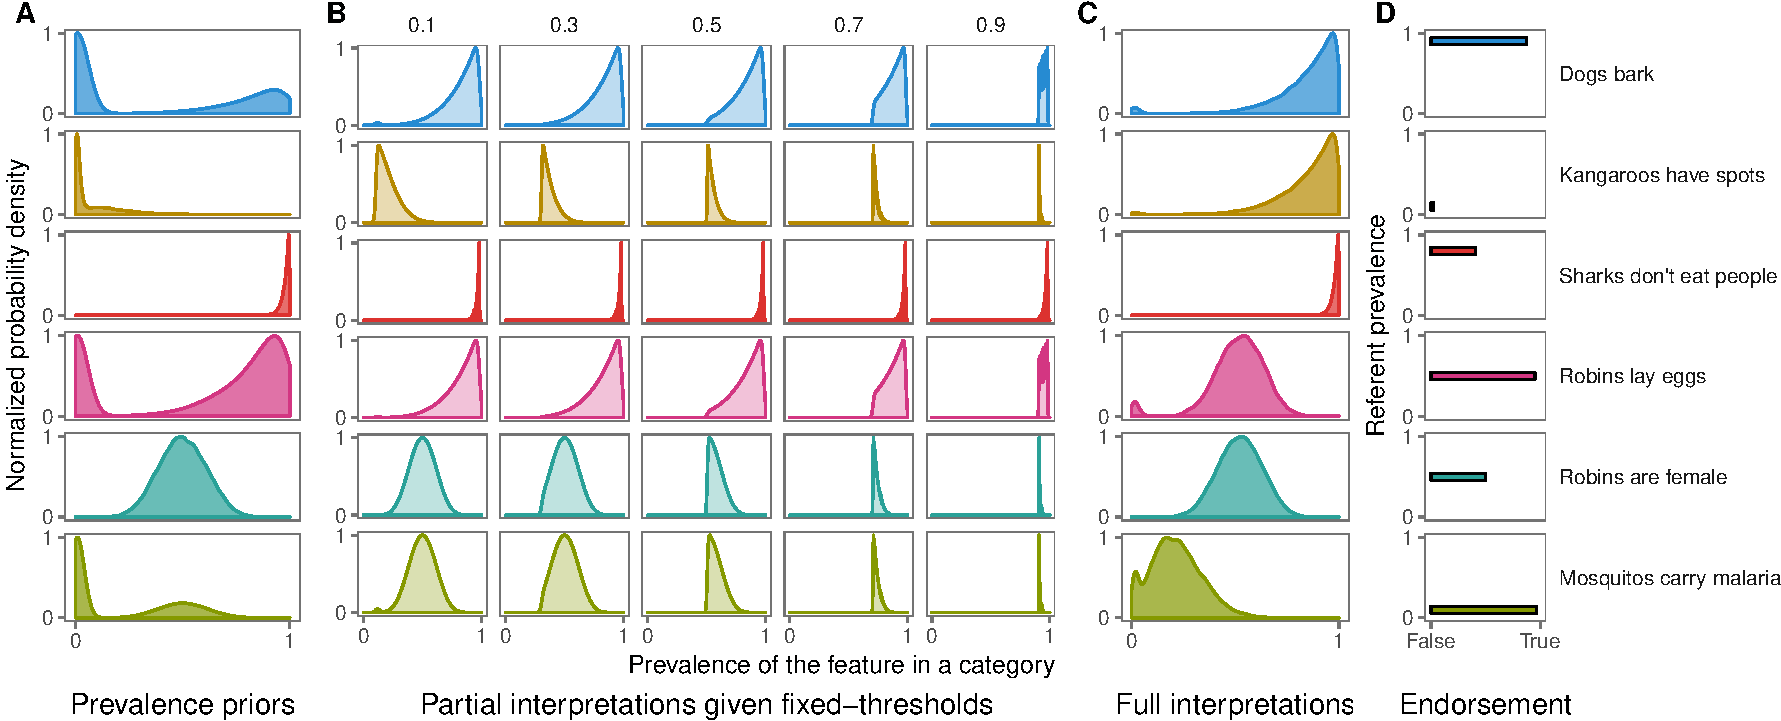
\includegraphics{figs/simulations-1.pdf}
\caption{\label{fig:simulations}Computational model behavior. A: Prior
distributions over the prevalence of a feature in a category for 6
example features B: Different fixed thresholds (columns) give rise to
different partial interpretations. C: The interpreter model averages
over all thresholds, producing posterior distributions that strongly
depend upon the priors. D: Endorsement model predictions, assuming a
particular referent-prevalence. Shapes of the priors were chosen to
intuitivly correspond to properties labeling the distributions.}
\end{figure}

The literal interpretation model computes a posterior distribution on
prevalence by considering different possible thresholds \(\theta\)
(Figure~\ref{fig:simulations}B). Low thresholds (e.g., \(\theta = 0.1\))
rule out very few possibilities (only \(p_{fk} \leq 0.1\)), and thus are
quite likely given that its consistent with much of the prevalence
prior. The flip-side of this is that the endorsement model is less
likely to produce an utterance with a low-threshold in mind, because the
end result would be similar to staying silent (a posterior not very
different from the prior). Higher thresholds (e.g., \(\theta = 0.9\))
rule out more possibilities and thus would be highly informative, but
the interpretation model must balance this with the prior probabilities
of the prevalences implied by the threshold
(Figure~\ref{fig:simulations}A).

The result of this reasoning process is a trade-off between highly
informative thresholds and the prior probabilities of the prevalences
implied by those thresholds. The prevalence-based interpretations of
generalizations of novel categories are shown in
Figure~\ref{fig:simulations}C. These interpretations depend heavily on
the prevalence priors (different rows). Hearing \enquote{Ks bark} tells
the literal interpretor that \emph{almost all} Ks bark, though there is
a good deal of uncertainty in the precise quantity (top row; pink).
\enquote{Ks lay eggs} has a strikingly different interpretation: It
means \enquote{Half of Ks lay eggs} (4th row; green). The literal
interpreter can also derive very weak interpretation, as shwon in the
\textsc{carries malaria} distribution (bottom row, purple).

The endorsement model (Eq. \ref{eq:S1}) predicts endorsement
probabilities based on the literal interpretation of the utterance and
the referent-category prevalence (e.g., how many robins lay eggs).
Predictions for a few classic examples from the generics literature are
shown in (Figure~\ref{fig:simulations}D). In accord with intuition, the
endorsement model predicts \enquote{Dogs bark}, \enquote{Robins lay
eggs}, and \enquote{Mosquitos carry malaria} are all true, despite the
referent-prevalences varying substantially between these three examples.
Intruigingly, the model predicts \enquote{Robins are female} (which has
the same prevalence as \enquote{Robins lay eggs}) should receive
intermediate endorsement: It is neither true nor false. To understand
this prediction, examine the interpretation distribution for the
\textsc{are female} distribution: It is identical with the prior
(Figure~\ref{fig:simulations} A vs.~C; blue distributions). The
endorsement model decides that is neither better nor worse to produce
the generalization than to stay silent, as they both carry the same
information content. This example can be contrasted with cases such as
\enquote{Sharks don't eat people} and \enquote{Kangaroos have spots},
which the model thinks would be misleading to say (i.e., better to say
nothing).

These simulations show how the model predicted endorsement depends upon
the background knowledge about the property \(P(p_f)\) as well as the
prevalence \(p_{fk}\) communicated. We chose schematic values for each
of these, and saw that the endorsement model recapitulates standard
intuitions about the truth or falsity of classic examples from the
generics literature. In what follows, we test this theory for a wide
range of generalizations, including generalizations of different types
(categories, events, and causes). We do this by both measurning and
manipulating background knowledge and referent-prevalence and relate it
to human elicited endorsements of generalizations.

\section{Case Study 1: Generic
Language}\label{case-study-1-generic-language}

Generalizations about categories (i.e., \emph{generic language}; e.g.,
\enquote{Dogs bark.}) have received substantial interest in psychology
for their role in concept and theory formation (e.g., Gelman, 2004),
stereotype propogation (Rhodes, Leslie, \& Tworek, 2012), and motivation
(Cimpian, Arce, Dweck, \& Markman, 2007), as well as many other facets
of everyday reasoning. In addition, generics have been the case study of
choice for the semantics of the language of generalization because of
their vexing similarity to quantified statements (e.g., \enquote{Most
dogs bark}). Time after time, psychologists have shown that generics
simply do not reduce to quantified statements (e.g., Khemlani et al.,
2012, Prasada et al. (2013), Cimpian, Brandone, and Gelman (2010)).

Here, we take our first empirical look at how the \emph{underspecified
threshold} endorsement model predicts actual human endorsements of
generic statements. We measure endorsement for thirty generic sentences
that cover a range of conceptual distinctions (Prasada et al., 2013):
\emph{majority characteristic} (e.g., \enquote{Ducks have wings.}),
\emph{minority characteristic} (e.g., \enquote{Robins lay eggs.}),
\emph{striking} (e.g. \enquote{Mosquitos carry malaria.}), \emph{false
generalization} (e.g., \enquote{Robins are female.}), and \emph{absent
features} (e.g. \enquote{Lions lay eggs.}). We further craft sentences
to elicit the full range of acceptability judgments (intuitively:
\enquote{true}, \enquote{false}, and \enquote{indeterminate}) for
generics with properties of low, medium, and high referent-prevalence
(Expt. 1a). We examine generics about animal categories in order to
reliably measure the prior belief distribution over the prevalence of
features \(P(h)\) (Expt. 1b). This elicitation procedure includes
measurements of the referent-category feature-probabilties \(h'\)
(e.g.,\(P(x \text{ lays eggs} \mid x \text{ is a robin})\)), allowing us
to both generate predictions for the endorsement model (Eq. \ref{eq:S1})
as well as for simpler, alternative models.

\subsection{Experiment 1a: Generic
endorsements}\label{experiment-1a-generic-endorsements}

In this experiment, we elicit human endorsements for generalizations
about categories (\emph{generics}) taken from the linguistic and
psychological literature on generics (Prasada et al., 2013). The goal of
this study is to observe a range of endorsements for generic statements
about animal categories.

\subsubsection{Method}\label{method}

\paragraph{Participants}\label{participants}

We recruited 100 participants over Amazon's crowd-sourcing platform
Mechanical Turk (MTurk). Participants were restricted to those with US
IP addresses and with at least a 95\% MTurk work approval rating (the
same criteria apply to all experiments reported). 4 participants were
excluded for failing to recall the button corresponding to
\emph{agreement} in the forced-choice task. 5 participants self-reported
a native language other than English; removing their data has no effect
on the results reported. The experiment took about 3 minutes and
participants were compensated \$0.35.

\paragraph{Procedure and materials}\label{procedure-and-materials}

Participants were shown thirty generic sentences in a randomized order.
They were asked to press one of two buttons (randomized
between-participants) to signify whether they agreed or disagreed with
the sentence (see Table 2 in Appendix for complete list). The thirty
sentences were presented in a random order between participants and
covered a range of conceptual categories described above. Approximately
10 true, 10 false, and 10 uncertain truth-value generics were selected.
All 30 generic sentences are shown in Figure
~\ref{fig:generics-endorsement-figure} A. As an attention check,
participants were asked at the end of the trials which button
corresponded to \enquote{Agree}. 4 participants were excluded for
failing this trial.

\subsubsection{Results}\label{results}

As a manipulation check, the first author assigned an \emph{a priori}
truth-judgment (true/false/indeterminate) to each stimulus item. As one
would expect, there were substantial differences in empirical
endorsements: true generics were almost universally endorsed (Maximum
A-Posteriori estimate and 95\% credible interval of endorsement
probability: \(0.93\) \([0.91, 0.94]\)); indeterminate generics were
agreed with \emph{less} likely than chance (\(0.38\) \([0.35, 0.42])\))
but substantially more than false generics (\(0.08\) \([0.06, 0.09])\)).

In addition to these categorical differences between our thirty generic
statements, we find a contiuum of endorsement values (Figure
~\ref{fig:generics-endorsement-figure} A). Such a continuum of judgments
is already evidence against any theory that only predicts categorically
whether a generic statement is true or false. Ideally, a complete theory
of genericity should be able to explain statements that are endorsed
completely, unendorsed completely, and all shades in between. We next
measure the prevalence prior distribution and articulate a set of formal
models that try to predict these endorsement data.

\subsection{Experiment 1b: Prevalence prior
elicitation}\label{experiment-1b-prevalence-prior-elicitation}

The prevalence prior \(P(h)\) in Eq. \ref{eq:L0} describes the belief
distribution on the probability of a given feature (e.g.,
\textsc{lays eggs}) across relevant categories. To get an intuition for
the kind of knowledge encoded in this belief distribution, consider the
following thought experiment: You are walking around and you come across
an instance of your favorite kind of animal from Earth (e.g., a
peregrine falcon). Ask yourself \enquote{is it female?} Your answer will
probably depend upon the percentage of the category that you believe to
be female (e.g., the percentage of female peregrine falcons, i.e.,
50\%). Now, do you think it lays eggs? Your answer to this question will
likely depend upon on what animal you're thinking of: If you're thinking
of a peregrine falcon, the probability is similar to that of being
female (50\%) because female peregrine falcons lay eggs; if you're
thinking of a mammal, it's likely that it won't lay eggs (0\%) because
most mammals give birth to live young. That is, the answer is roughly
either 50\% or 0\% depending on the kind of creature you are thinking
of\footnote{The subjective probability may, in fact, be non-zero and
  small as opposed to 0. Non-zero probabilities allow for the intuitive
  possibility of a dog that lays eggs potentially due to some strange
  generic mutation or the interaction of dog genetics with a strange
  environment.}.

This thought experiment decomposes the prevalence prior \(P(h)\) into a
prior distribution on kinds \(P(k)\) and then a conditional probability
of the prevalence given the kind \(P(h \mid k)\). We will use this
decomposition to measure the prevalence prior
\(P(h) = \int_{k} P(h \mid k) \diff k\) and perform Bayesian data
analysis to accurately reconstruct the prevalence prior. We measured
prior distributions empirically for the set of properties (e.g.,
\textsc{lays eggs, carries malaria}; 21 in total) used in our generic
sentences in Expt. 1a. To create a larger set of properties, we
reverse-code responses for five properties to create their corresponding
negative properties (e.g., we create a property \enquote{doesn't have
beautiful feathers} by subtracting from 100\% the responses for
\enquote{has beautiful feathers}).

\subsubsection{Method}\label{method-1}

\paragraph{Participants}\label{participants-1}

We recruited 60 participants over Amazon MTurk.\\
3 participants were accidentally allowed to complete the experiment for
a second time, so we excluded their second responses (resulting in
\(n=57\)). 2 participants self-reported a native language other than
English; removing their data (\(n=55\)) has no effect on the results
reported. The experiment took about 10 minutes and participants were
compensated \$1.00.

\paragraph{Procedure and materials}\label{procedure-and-materials-1}

On each trial of the experiment, participants filled out a table where
each row was an animal category and each column was a property.
Participants first were shown six animal categories randomly sampled
from a set corresponding to referent-categories of the generic sentences
used in Expt. 1a (e.g., \textsc{robins, mosquitos}) and were asked to
generate five of their own (Figure ~\ref{fig:generics-prior-task} A). A
column then appeared to the right of the animal names with a property
label in the column header (e.g., \emph{lays eggs}). Participants were
asked to fill in each row with the percentage of members of each of the
species that had the property by giving a number (e.g., \enquote{50\%};
Figure ~\ref{fig:generics-prior-task} B). Eight property--columns in
total appeared in the table.

This whole procedure was repeated two times (two trials). In total, each
participant generated ten animal names and reported on the prevalence of
sixteen properties for twenty-two animals (their own ten and the
experimentally-supplied twelve).

\begin{figure}[htbp]
\centering
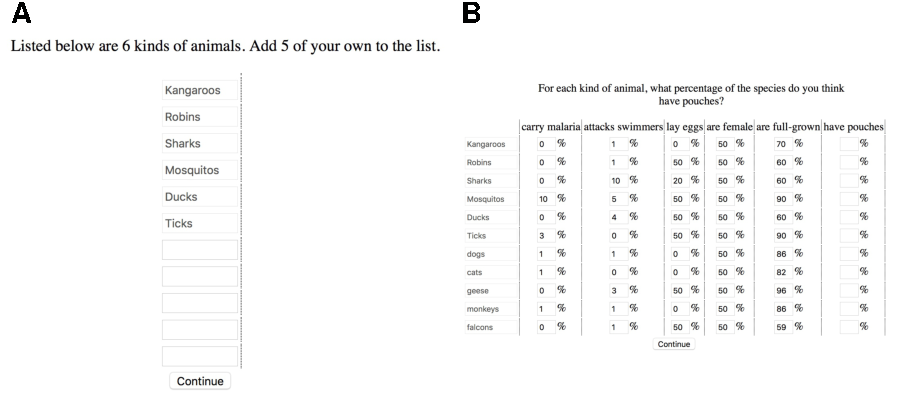
\includegraphics{figs/generics-prior-task-1.pdf}
\caption{\label{fig:generics-prior-task}Prior elicitation task. A:
Participants first generated animal names after seeing six example
categories. B: One feature at a time, participants estimated the
percentage of the category with the feature, for each category.}
\end{figure}

\subsubsection{Qualitative results}\label{qualitative-results}

There is a lot of diversity in the shapes of the elicited prior
distributions (8 examples shown in Figure~
\ref{fig:generic-endorsement-priors-figure} A), which is roughly
consistent with the schematic prior distributions used in the
\emph{Model Simulations} section (Figure ~ \ref{fig:simulations} A). The
property \emph{being female} is present in almost all categories in
almost exactly the same proportion, where as properties such as
\emph{laying eggs} or \emph{having spots} exhibit more structure
represented by the multimodality of these distributions. \emph{Being
red} exists mostly at extremely low prevalence levels (i.e., 0
prevalence) but also at high prevalence levels (e.g., 50\% or 100\%),
whereas \emph{carrying malaria} is really only present at low prevalence
levels. This diversity is important because the endorsement model makes
different predictions depending on the shape of the prior.

\subsubsection{Quantitative modeling}\label{quantitative-modeling}

In order to integrate the results of this prior measurement task into
our model of endorsement, we must accurately model the prior elicitation
data. We do this using a Bayesian mixture model, which assumes that the
data generated for each property (e.g., \textsc{lay eggs}) comes from
one of two underlying Beta distributions (\emph{Mixture of
Betas}).\footnote{The Beta distribution is chosen because the support of
  this distribution is numerical values between 0 - 1, exactly the form
  of the response data in the prior elicitation task.} We specify one of
these distributions \emph{a priori} to represent kinds of animals who
\emph{do not have} a stable causal mechanism that could give rise to the
property (e.g., \textsc{lions} and \textsc{lay eggs}), which results in
prevalence or prevalence values close to or equal to 0.\footnote{This
  assumption is similar in spirit that employed by \emph{Hurdle Models}
  of epidemiological data, where the observed count of zeros is often
  substantially greater than one would expect from standard models, such
  as the Poisson (e.g., when modeling adverse reactions to vaccines;
  Rose, Martin, Wannemuehler, \& Plikaytis, 2006)} This \enquote{null
distribution} is potentially present for all features in exactly the
same way (i.e., the lack of producing the feature). The second
distribution represents kinds of animals who \emph{do have} such a
mechanism, and the two parameters of this distribution are not specified
\emph{a priori} and are not the same for all properties, but are
inferred on a property-wise basis from participants' responses. The
\emph{Mixture of Betas} distribution has a third free parameter (for
each property), the relative contribution of the \enquote{null
distribution} (for example: we expect the \enquote{null distribution} to
not contribute at all to properties like \emph{being female}, for which
almost all categories have at least some members with the property). To
ensure the \emph{Mixture of Betas} model of the prior is not overly
complex, we fit an additional model that represents only a single
underlying distribution (\emph{Single Beta}) for a comparison. For more
details about model implementation and inference, see Appendix C.

The prior distributions over prevalence are well modeled as a mixture of
two Beta distributions and not as a single Beta distribution (Figure~
\ref{fig:generic-endorsement-priors-figure} B; red vs.~blue lines). The
\emph{Single Beta} model does okay for the \emph{being female}
distribution, but overly smooths the other distributions, washing out
the latent structure in participants' responses. One prior that the
\emph{mixture of Betas} model does not perfectly capture is the prior
distribution over the feature \textsc{lay eggs}. The empirical
distribution is tri-modal, with reliable modes at 0\%, 50\%, and
100\%\footnote{Similar phenomena have been observed in other prevalence
  elicitation tasks when the referent-category is fixed (e.g.,
  estimating only the percentage of \emph{robins} that \emph{lay eggs};
  Prasada et al., 2013)}; a simple two-component mixture model has no
way to account for such a tri-modal distribution. A more complex model
(i.e., one with three mixture components) is necessary to perfectly
account for this item.

\begin{figure}[htbp]
\centering
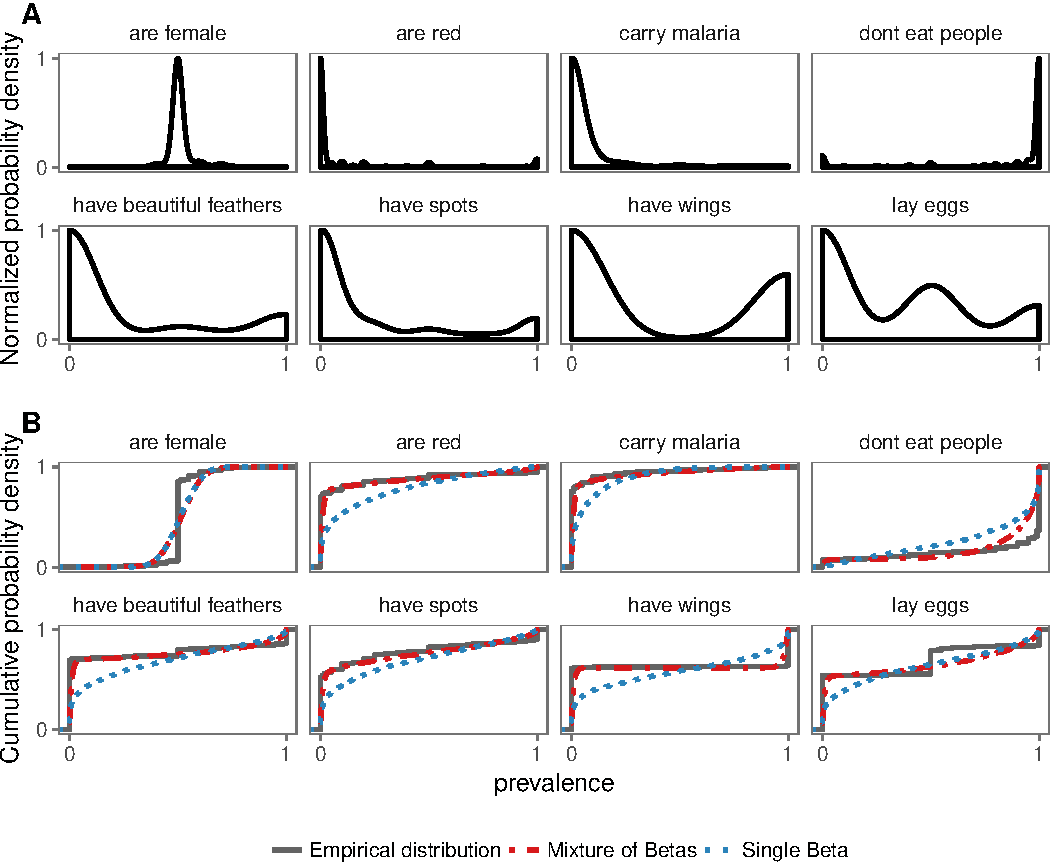
\includegraphics{figs/generic-endorsement-priors-figure-1.pdf}
\caption{\label{fig:generic-endorsement-priors-figure}A: Empirically
elicited prior distributions over prevalence for eight properties. B:
Cumulative density plots reveal that a model of a mixture of two Beta
distributions does substantially better at capturing the structure of
the priors than a single Beta distribution. Distributions are the
posterior predictive distributions for the models of the prio and the
raw empirical distribution. A completely uniform distribution would be
represented as the y = x line.}
\end{figure}

\subsection{Endorsement model
comparison}\label{endorsement-model-comparison}

To understand the generative process of generic endorsement, we
articulate a set of formal models that have been previously-proposed in
the literature, an alternative-form of our proposed endorsement model,
and our full endorsement model. As the simplest baseline hypothesis, we
first explore how well referent-category prevalence itself predicts
generic endorsement (e.g., does the fraction of \textsc{robins} that
\textsc{lay eggs} predict the felicity of \emph{Robins lay eggs}?). As a
secondary alternative hypothesis, we explore whether referent prevalence
and \emph{cue validity}---the probability of a kind given the feature
(described in more detail below)---predicts the endorsement data. We fit
these models using standard maximum-likelihood techniques; we model
uncertainty in the input measurements (i.e., referent prevalence, cue
validity) by bootstrapping those data.

Our underspecified-threshold hypothesis models endorsement by
considering how well the generalization would bring a naive
interpreter's prior distribution on prevalence \(P(h)\) (e.g., the
prevalence of laying eggs among other animals) in line with the
referent-category prevalence (e.g, the prevalence of laying eggs among
robins). There are several substantive components to this hypothesis:
(a) the prior distribution \(P(h)\) is relevant, (b) endorsement is a
decision-theoretic process of uttering the generalization vs.~not
uttering it, and (c) the core semantics of a generalization is an
uncertain threshold. As a control model, we assign a fixed semantics to
the generalization (i.e., analogous to the quantified statements) but
keep the prior and the decision-theoretic architecture in place. This
provides a strict test of the uncertain-threshold hypothesis (c).

\subsubsection{Baseline models}\label{baseline-models}

\paragraph{Referent prevalence}\label{referent-prevalence}

From the prevalence prior data (Expt. 1b), we estimate participants'
beliefs about the probability of a feature for the referent categories
(e.g., the percentage of \textsc{robins} that \textsc{lay eggs}). We
find a little over half of the variance in the endorsement data is
explained this way (\(r^2(30) = 0.51\); MSE=\(0.08\); Figure ~
\ref{fig:generic-endorsement-priors-figure}, upper-right: lower-left
facet). The referent prevalence baseline is a decent model of these data
because our stimulus set includes generics that are true with high
prevalence properties (e.g., \emph{Leopards have spots.}) and generics
that are false with low prevalence properties (e.g., \emph{Leopards have
wings.}).

However, large deviations from an account based purely on referent
prevalence remain: Generics in which the referent-category has
intermediate prevalence (prevalence quartiles 2 and 3:
\(16\% < \text{prevalence} < 64\%\)), are not at all explained by
referent prevalence (\(r_{Q2,3}^2(15) = 0.01\); MSE = \(0.14\)). This
includes generics that are judged true with relatively low referent
prevalence (e.g., \enquote{Mosquitos carry malaria}) and false with
relatively high referent prevalence (e.g., \enquote{Sharks don't eat
people}).

\paragraph{Cue validity and referent
prevalence}\label{cue-validity-and-referent-prevalence}

\subparagraph{Model specification}\label{model-specification}

Cue validity is linearly related to a point-estimate of the prevalence
prior distribution (see Model section and Appendix A). It thus
implicitly captures information about other categories, though cannot
capture the structure that is present in the prevalence priors. To show
that this structure is important, we explore a secondary baseline model
based on prevalence and cue validity.

Though the cue validity of a particular (category, property) pair can be
derived from the prevalence prior distribution, previous empirical
studies of generic language have not done this. Instead, these studies
estimate cue validity by asking a separate group of participants about
the distinctiveness of features for given animals (e.g., Khemlani et
al., 2012), though different studies use different measurements.
Preliminary analysis of these different measurements revealed that a
\emph{free production} paradigm (Cree, McNorgan, \& McRae, 2006) is
preferred. Participants (\(n = 100\)) were supplied with a feature
(e.g., \enquote{X lays eggs}) and asked to generate a kind (e.g.,
\enquote{what do you think X is ?}). For a detailed analysis of
different cue validity measurements and comparison to \emph{prevalence
prior derived cue validity}, see Appendix B.

\subparagraph{Results}\label{results-1}

A linear model that uses predictors for both referent-prevalence and cue
validity does a better job at explaning the endorsement data than just
prevalence alone (\(r^2(30) = 0.73\); MSE=\(0.04\)). This model is able
to account for the endorsements of examples like \enquote{Mosquitos
carry malaria} (model endorsement and bootstrapped-95\% confidence
interval = 0.84 {[}0.72, 0.92{]}) and \enquote{Lions have manes} (0.79
{[}0.63, 0.88{]})), as these features are very diagnostic of the kind
(human endorsement both \(> 0.9\)). Deviations, however, still remain.
For example, \enquote{Robins lay eggs} still receives only intermediate
endorsement by this model (0.68 {[}0.57, 0.79{]}; human endorsement =
0.94 {[}0.87, 0.97{]}), and \enquote{Mosquitos don't carry malaria} is
judged to be a pretty good statement (0.57 {[}0.42, 0.71{]}; human
endorsement = 0.07 {[}0.04, 0.14{]}).

\enquote{Robins lay eggs} and \enquote{Mosquitos don't carry malaria}
highlight a shortcoming of reducing structured prevalence prior
distributions to single point-estimates of cue validity. \enquote{Lays
eggs} is a somewhat diagnostic feature for \emph{birds}, but there are
many kinds of birds, and the feature is not itself diagnostic for a
particular kind of bird like \enquote{Robins}. Thus, the cue validity is
low even though robins are in the distinctive part of the \enquote{lays
eggs} prevalence prior distribution (e.g., Fig.~\ref{fig:simulations}A
bottom). Furthermore, cue validity glosses over the difference between
\enquote{undiagnostic} features (features present in almost every
category; e.g., \enquote{not carrying malaria}) and \enquote{false}
features (features that are absent a particular category; e.g.,
\enquote{lions} and \enquote{lay eggs}; see Appendix B for more
discussion of this distinction). Such a model makes the wrong prediction
for non-distinctive properties that in, absolute terms, have high
prevalence but in relative terms, low prevalence (e.g.,
\enquote{Mosquitos don't carry malaria}). A simple metric like cue
validity is too blunt to capture these subtleties.

\subsubsection{Communicative endorsement
models}\label{communicative-endorsement-models}

The model we propose for endorsing generalizations is a model of an
agent that decides whether or not to say the generalization to a naive
interpretor. The endorsement model (Eq. \ref{eq:S1}) decides whether or
not to assert the generalization to a naive interpretor (Eq.
\ref{eq:L0}) conditioned on a particular referent-category prevalence
\(h'\) (e.g., the percentage of robins that lay eggs). We use the
empirically estimated referent-category prevalence (the same as used in
the baseline regression model) as the referent-category prevalence
\(h'\) in the endorsement model. The empirically measured priors from
Expt. 1b are used as the literal interpreter's prevalence prior
\(P(h)\).

To incorporate the measurements of these model components into our
endorsement model, we build a single, Bayesian joint-inference model of
the referent-category prevalence \(h'\), prevalence priors \(P(h)\)
(both from Expt. 1b data), and the endorsement data (Expt. 1a). Modeling
the data from both Expt. 1a and 1b by a single, joint-inference model
simultaneously makes explicit our assumptions about how these data were
generated and is the proper way to represent the uncertainty in our
measurement of the prior elicitation data (see Appendix and Figure~
\ref{fig:genericsModelDiagram} for further model specification details).
The endorsement model is then fully specified after setting the single
optimality parameter \(\lambda_1\) (in Eq. \ref{eq:S1}). To learn about
the credible values of the parameters of the model and resulting model
predictions, we ran an incrementalized version of MCMC (Ritchie,
Stuhlmüller, \& Goodman, 2016) for 3 chains of 100,000 iterations,
discarding the first 50,000 for burnin.

The number of parameters of this full data-analytic model is relatively
large, and thus there is a concern that the parameters themselves (as
opposed to the exact structure of our model) are doing the work. To
address this concern, we construct a strong, alternative model that uses
the same data analytic strategy and only differs in the uncertain
semantic threshold \(\theta\) is replaced with a fixed-threshold. To
provide the strongest possible test, we make the fixed-threshold a
parameter of the data-analytic model, to search for the best possible
fixed-threshold. Finally, a fixed-threshold model will have to
accomodate responses that are inconsistent with the threshold (i.e., a
participant endorsing the generalization when the referent prevalence is
low); we thus outfit this model with an \emph{additional} noise
parameter, to allow for random guessing. Thus, our fixed-threshold
alternative model says that participants make an information-theoretic
decision, taking into account the interpreter's prior distribution
\(P(h)\), using a fixed-threshold semantics, where deviations from a
pure information-theoretic decision are accounted for by noise. This
alternative model has 2 additional parameters to our uncertain threshold
model (the fixed-threshold and the proportion of noise responses). We
examine the predictions of this alternative model first.

\paragraph{Fixed-threshold with noise
model}\label{fixed-threshold-with-noise-model}

\begin{figure}[htbp]
\centering
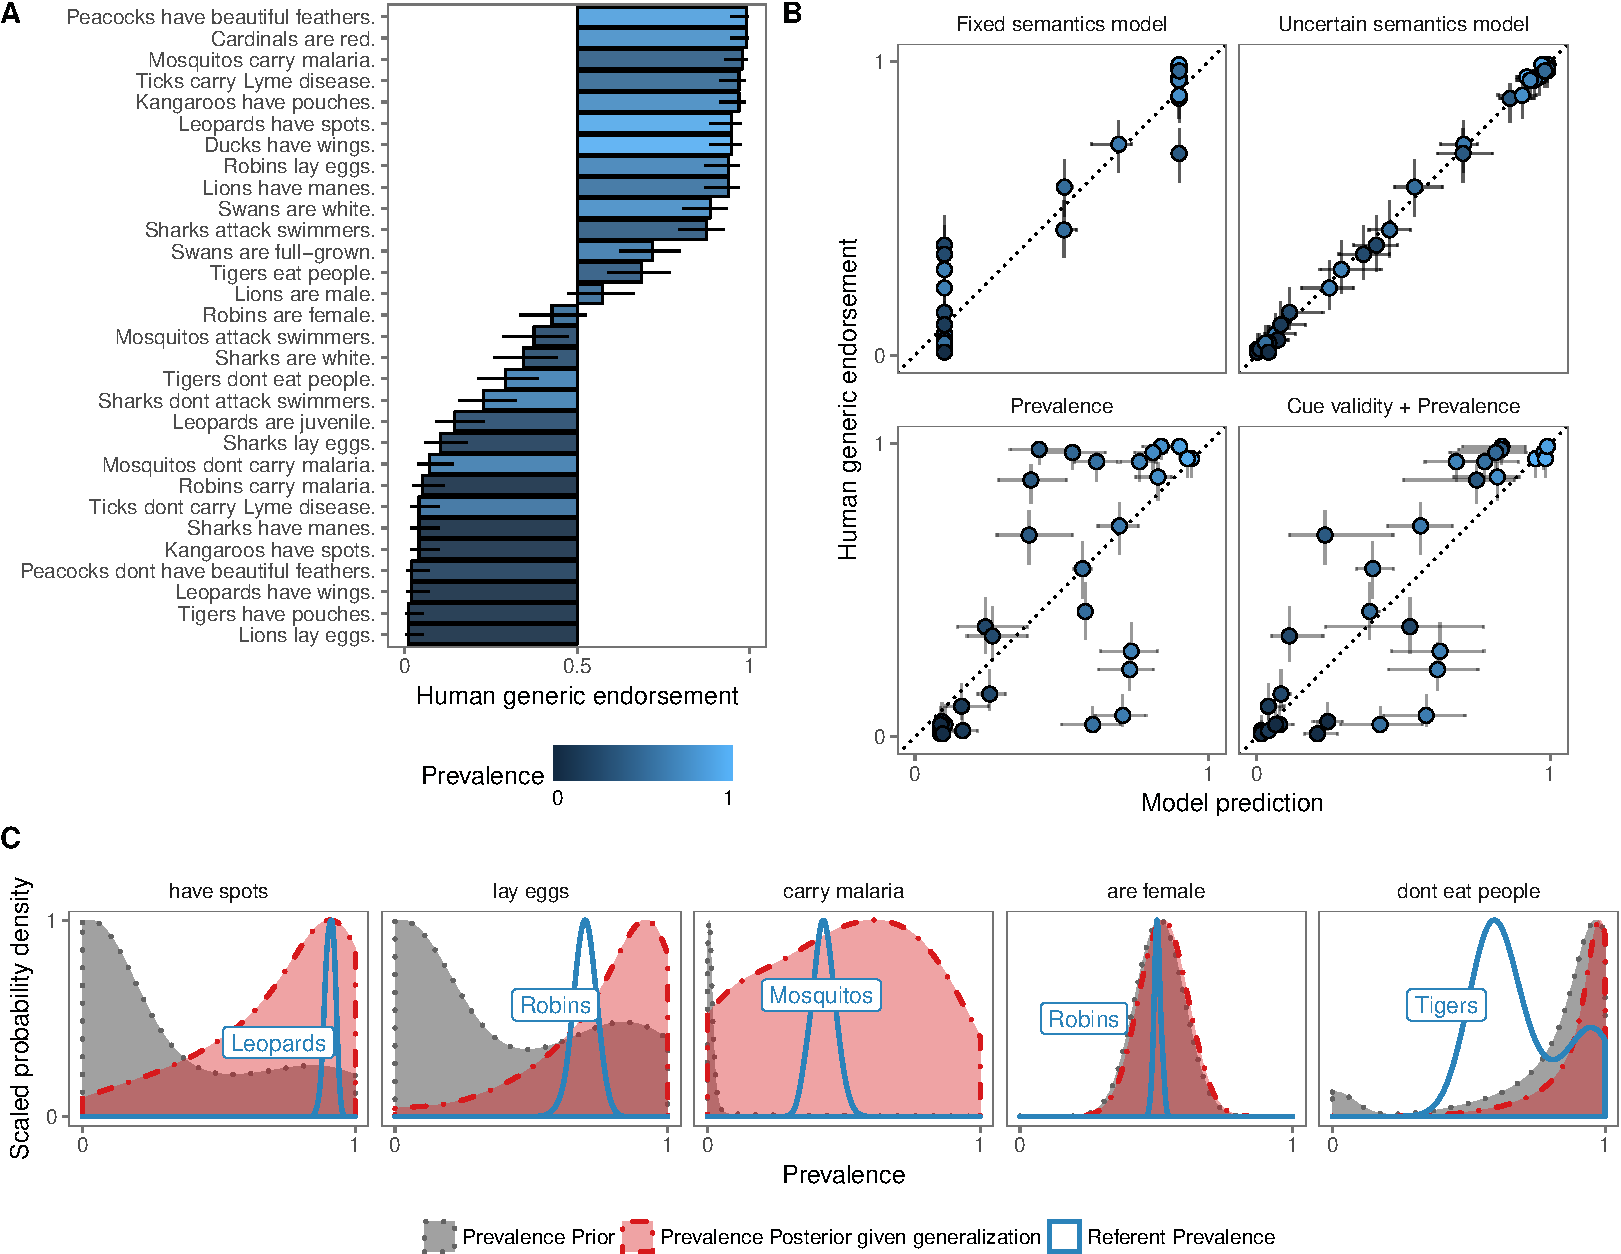
\includegraphics{figs/generics-endorsement-figure-1.pdf}
\caption{\label{fig:generics-endorsement-figure}Endorsing generalizations
about categories. Top left: Human elicited endorsements for thirty
generic sentences reveal a continuuum of endorsements. Top right: Model
fits for the uncertain semantics speaker model (upper right), a fixed
semantics speaker model (upper left), and regression models based on
referent prevalence alone (lower left) and prevalence + cue validity
(lower right). Bottom: Five example prevalence priors, listener
posteriors upon hearing the generalization, and speaker belief
distributions about the referent prevalence. These distributions are
inferred using all three data sources from Expt. 1 (see Figure
\ref{fig:genericsModelDiagram} for an overview of the Bayesian data
analytic approach).}
\end{figure}

To evaluate the fixed-threhsold model, we examine the posterior
distribution which represents what we should believe about the latent
parameters of the model (referent prevalence, prevalence priors, the
optimality, fixed-threshold, and noise parameters) given the observed
data, as well as what predictions of the model given these parameter
values. The Maximum A-Posteriori value and 95\% highest probability
density interval for the inferred (fixed) threshold and noise parameters
are 0.34 {[}0.25, 0.37{]} and 0.20 {[}0.18, 0.22{]}, respectively. The
inferred optimality parameter in Eq. \ref{eq:S1} is 0.34 {[}0.25,
0.37{]}.

We compare the fixed-threshold model's posterior predictive distribution
of generic endorsement to the empirical truth judgments. Figure
\ref{fig:generics-endorsement-figure} (top right; top left subplot)
shows the fixed-threshold model's ability to predict the generic
endorsement data (\(r^2(30) = 0.9329\); MSE = \(0.010964\)). Though the
model is able to capture a lot of the variance, it only makes three
kinds of judgments: true, false, or neither. It treats \enquote{Tigers
eat people} (0.90 {[}0.85, 0.91{]}) as good a statement as
\enquote{Peacocks have beautiful feathers} (0.88 {[}0.85, 0.91{]}),
though participants seem to give a substantially weaker endorsement of
the former (\enquote{Tigers eat people} = 0.69 {[}0.59, 0.77{]};
\enquote{Peacocks have beautiful feathers} = 0.99 {[}0.94, 1{]}).
Similarly, \enquote{Lions lay eggs} is judged to be just as bad as
\enquote{Mosquitos attack swimmers}(0.10 {[}0.09, 0.15, 0.10 {[}0.09,
0.15{]}, respectively), though participants rate the former as
completely false (0.01 {[}0, 0.06{]}) while the latter is kind of true
(0.38 {[}0.28, 0.48{]}). This alternative model is unable to make these
fine-grained distinctions because it must use the same semantic
threshold in all contexts.

\paragraph{Uncertain threshold model}\label{uncertain-threshold-model}

Our underspecified threshold model is the same as the fixed-threshold
model, except that rather than having a fixed \(\theta\) for all
contexts, the model infers context-specific \(\theta\)'s. We construct
the same joint-inference Bayesian data analytic model as we did for the
fixed-threshold analysis; however, we are able to drop the additional
parameters required for the fixed-threshold model (the fixed-threshold
and noise parameters). Thus, this model has two \emph{fewer} parameters
than the fixed-threshold model above.

We first examine the posterior predictive distribution on the prevalence
prior and referent-prevalence data to ensure that the joint-inference
model fits these data as well as the Bayesian model that modeled these
data in isolation. This is an important step in model validation because
it tells us that our model's predictions are derived from reasonable
values of the parameters. Importantly, the model recapitulates the prior
elicitation data (e.g., the probability of laying eggs among various
species) and the referent-category prevalence data (e.g., the
probability of laying eggs among robins) as it did when the Bayesian
data analysis model only included these data and their associated model
(results section of Expt. 1b). This result confirms that the
theoretically-interesting predictions of this model --- predictions of
generic endorsement --- are based on intuitively meaningful model
components (i.e., the shapes of the prevalence distributions).

The inferred optimality parameter in Eq. \ref{eq:S1} is 0.34 {[}0.25,
0.37{]}.

As we see in Figure ~\ref{fig:generics-endorsement-figure} (top right,
top right subplot), the endorsement model that uses an
uncertain-threshold semantics explains nearly all of the variance in
human endorsements (\(r^2(30) = 0.9978\); MSE = \(0.00035185\)). To gain
some intuition for why that is the case, examine the bottom row of
Figure \ref{fig:generics-endorsement-figure}. The blue, solid lined
distribution corresponds to the speaker's beliefs about the probability
of the feature for the referent-category (i.e., \emph{referent
prevalence}). The grey distribution shows the listener's prior
distribution over probabilities of the feature (these are the
corresponding Probability Density Functions of the Cumulative Density
Functions shown in Figure ~\ref{fig:generic-endorsement-priors-figure}.
It is also the listener \(L_0\)'s posterior on referent prevalence upon
hearing the silent utterance. The red distribution shows the \(L_0\)
posterior upon hearing the generic utterance that corresponding to an
uncertain threshold-semantics. The speaker model decides when the
generic utterance conveys information that would bring the listener's
distribution more in line with the speaker's own distrubtion. Thus, it
finds that \enquote{Leopards have spots}, \enquote{Robins lay eggs}, and
\enquote{Mosquitos carry malaria} are also useful things to say.
\enquote{Robins are female} is neither good nor bad, as the
information-content of the utterance is very small relative to silence.
\enquote{Tigers don't eat people} is rather misleading, however; it
doesn't bring the listener closer to the speaker's distribution, despite
the speaker believing that the prevalence is more than half.

\subsection{Discussion}\label{discussion}

Generic language is the premier case study for generalizations in
language. Generics have been studied extensively in the cognitive and
developmental psychological literatures and shown to have deep
implications for wide ranging phenomena from stereotype propogation
(Rhodes et al., 2012) to motivation (Cimpian et al., 2007). Heretofore,
however, no formal model has been able to pass the most basic
truth-functional tests of the semantics of generalizations, knowing when
they are true and false. Determining the truth conditions is the first
step towards articulating a formal theory of how the language updates
beliefs.

We have demonstrated that a semantics based on the probability of the
feature is tenable in spite of alleged counterexamples. The key
theoretical insight is that the truth-functional semantics is
\emph{underspecified} yet still is able to formalize, using recent
developments in probabilistic modeling. Our model provides a clean
delineation of world knowledge (formalized as a prior distribution) from
the semantics of generalizations. We return to this point, and its
implications for theory-building, in the general discussion.

In explaining the variable endorsements of generics, we related the
referent-category prevalence (e.g., the percentage of robins that lay
eggs) to the endorsement of the generalization (e.g., \enquote{Robins
lay eggs}) via the prevalence priors (e.g., the percentage of different
kinds of animals that lay eggs). In doing so, we used generic statements
about familiar animal categories, which has long been the cleanest
domain for testing semantic theories of generics by providing minimal
comparison like \enquote{Robins lay eggs} vs. \enquote{\ldots{} are
female}. To model statements about familiar categories, we were forced
to \emph{measure} the relevant quantities in the model (i.e., the
referent prevalence and the prevalence priors), which people have access
to via their mental representations of the category. We now seek to
demonstrate how these quantities are causally related to endorsement, by
manipulating referent prevalence (Case 2) and feature-probabilitiy
priors (Case 3). In addition, we take this opportunty to highlight the
generality of the theory, by performing these additional empirical tests
in different domains for generalization: events and causes.

\section{Case Study 2: Habitual
Language}\label{case-study-2-habitual-language}

The event of Mary smoking at 2:30pm on January the 24th is an instance
of a kind of event: \emph{Mary smoking}. Just as with categories,
generalization can occur over events of a particular type. When
expressed in language, these generalizations take the form of
\emph{habitual language}: \enquote{Mary smokes}.

Events are a broad class of entities. In our second case study, we focus
on habituals about people's behaviors that take the form:
\textsc{singular noun phrase} \(+\)
\textsc{present tense simple verb phrase} (e.g., \enquote{Mary smokes
cigarettes}). Learning about the behaviors of others is useful because
they tell us about what that person is like more generally (e.g.,
Repacholi \& Gopnik, 1997; Seiver, Gopnik, \& Goodman, 2013). When
children describe their lives to other, a surprisingly large amount of
the langauge produced concerns the actions of people close to them
(e.g., ``My brother works part-time at the restaurant''; W. J. McGuire
\& McGuire, 1986). Habitual language about people may be a more
conservative form of \emph{trait language} (e.g., \enquote{Mary is a
smoker.}) and convey that behaviors are relatively enduring (Gelman,
2004; Gelman \& Heyman, 1999).

To test the generality of our theory, we use the same computational
model and follow the same general experimental structure as in the first
case study. We take event analogue of prevalence to be the \emph{rate}
with which the event occurs (e.g., how often Mary smokes). For the
generalization \enquote{Mary smokes}, instances of the category being
generalized are \emph{instances of Mary} and if for the instance to have
the feature, it means the instance of Mary is one in which she is
smoking. We test this by first measuring the prevalence (rate) prior
distribution for various actions (e.g., how often different people smoke
cigarttes; Expt. 2a). We then measure endorsements of habitual
statements while manipulating the \emph{referent-prevalence} (Expt. 2b),
and use our computational model to predict habitual endorsements. By
describing novel characters to participants, we are able to directly the
manipulate the \emph{referent-prevalence} (rate), which we were unable
to do for generalizations about familiar categories.

Finally, if habituals (and generics) are truly language for conveying
generalizations, it would be useful for them to reflect a speaker's
expectations, not merely her observations. Our computational model
predicts endorsement rates given a referent-prevalence \(p_{fk}\). Does
prevalence represent the actual, past frequency of the event (e.g., how
often Mary has actually smoked in the past month) or the predictive
probability of the event in the near future (e.g., how often we should
expect Mary to smoke next week)? We extend our theory by measuring
participants' predictions about future rates and endorsements of
habituals when causal forces intervene on the world (Expt. 2c). We then
use our model to test whether habitual endorsements are based on past
frequencies or future expectations.

\subsection{Experiment 2a: Measuring the prevalence prior for
events}\label{experiment-2a-measuring-the-prevalence-prior-for-events}

In order to generate model predictions for corresponding habitual
statement, we first elicit the prior distributions over rates for
different events. For language about the behaviors of people, \(P(p_f)\)
represents a language user's background knowledge about the rates with
which people do a behavior; this prior can be constructed as a
distribution over \emph{different people}, each of whom do the behavior
with a different rate. We designed our elicitation task to take
advantage of the mixture-model representation of the prevalence prior
used in Expt. 1 . In particular, we assume, to a first approximation,
that the distribution over prevalence can be represented as a mixture of
those who tend to do the action with a stable rate and those who do
not.\footnote{In the case of event knowledge about people, we expect
  there to be several more than just these two possibilities represented
  in the prior, corresponding to individuals with different traits or
  demographics. We assume here a simple structure so as to not make the
  specification of the prior overly complex.} With the further
assumption that, all else being equal, past is predictive of future
behavior, we operationalize these two kinds of people as \emph{people
who have done the action before} and \emph{people who have not the
action before}. We design this experiment to measure participants'
beliefs about the relative proportion of these two kinds of people (as a
measure of the mixture parameter in the model) as well as the rate at
which people (who have done the action before) do the action (as a
measure of the mean of stable-rate people). We will aassume for
simplicity that people who have never done the action before will rarely
or never do the action.

\subsubsection{Method}\label{method-2}

\paragraph{Participants}\label{participants-2}

We recruited 40 participants from Amazon's Mechanical Turk. Participants
were restricted to those with U.S. IP addresses and who had at least a
95\% work approval rating. The experiment took on average 12 minutes and
participants were compensated \$1.25 for their work.

\paragraph{Materials}\label{materials}

To construct our stimulus set, we choose actions from five categories of
typical human behaviors: eating/consuming food and drug, work, wearing
clothing, entertaining activities, and hobbies. For each category, we
created pairs or triplets of events that shared a superordinate actions
(e.g. \emph{writing} poems vs.~novels). The events were chosen to
intuitively cover a range of likely frequencies. In total, thirty-one
events were used. For a full list the stimulus set, see Appendix D.

\paragraph{Procedure}\label{procedure}

For each event, participants were asked two questions, with different
dependent measures. These questions were designed to measure the two
central components of the prevalence prior model. We anticipated there
to be different beliefs about the rates and relative proportions of
peopel depending on whether an actor is male or female, so we asked
about both genders separately.

\begin{enumerate}
\item ``How many \{men, women\} have \textsc{done action} before?'' \\

Participants responded ``N out of every J.'' by entering a number for N and choosing J from a drop-down menu (options: \{1000 - 10 million\}, incremented by 10x; default setting: 1000).

\item ``For a typical \{man, woman\} who has \textsc{done action}  before, how frequently does he or she \textsc{do action}?''\\  

Participants responded ``M times in K.'' by entering a number for M and choosing K from a drop-down menu (options: \{week, month, year, 5 years\}; default setting: year).
\end{enumerate}

For example, one set of prompts read: \enquote{How many women have
smoked cigarettes before?}; \enquote{For a typical woman who has smoked
cigarettes before, how frequently does she smoke cigarettes?}
Participants answered both questions for both genders on each slide (4
questions total per slide, order of male / female randomized
between-subjects), and every participant completed all 31 items in a
randomized order. The difference in meaning of these questions was
explained to participants on an instructions page before the
experimental trials and tested for recall on a subsequent trial.
Participants responded to this attention check by selecting an option
from a drop-down menu consisting of four options (one correct
description of the questions and three distractors).

\begin{figure}[htbp]
\centering
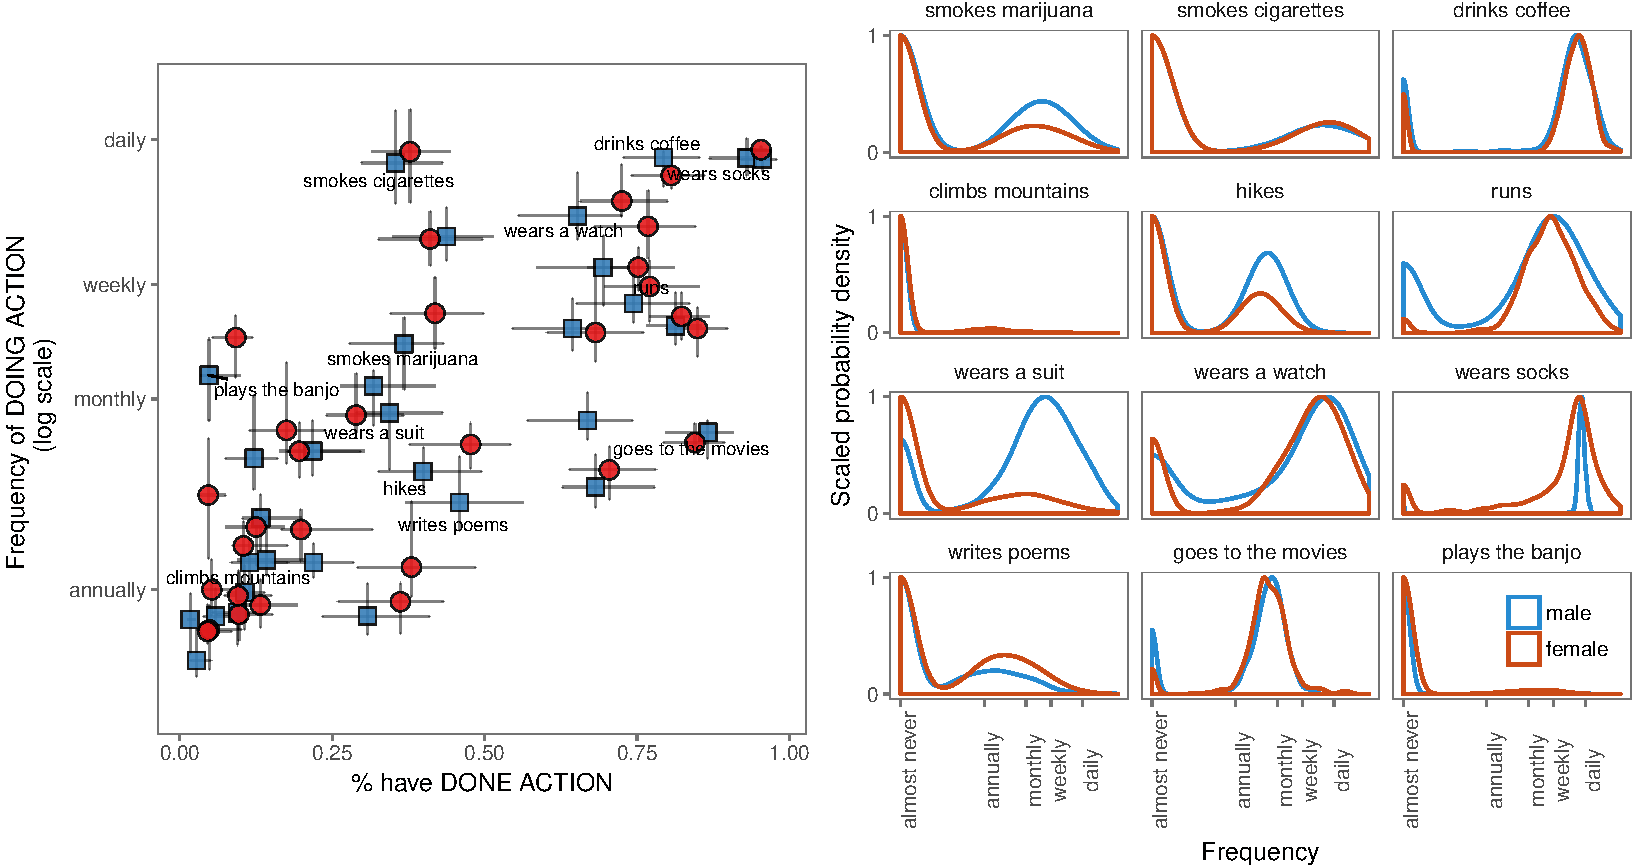
\includegraphics{figs/habituals-prior-figure-1.pdf}
\caption{\label{fig:habituals-prior-figure}Prevalence priors for events
(Expt. 2a). Left: Mean mixture parameter and mean stable frequency
parameter for 31 events. Right: Inferred priors on frequencies from the
structured, prior elicitation task. Priors are reconstructed by forward
sampling using the inferred parameters in the prior mixture model.}
\end{figure}

\subsubsection{Data analysis and
results}\label{data-analysis-and-results}

All participants responded correctly to both questions in the attention
check trial, so all collected data was used in the analysis. Question 1
elicits the proportion of people who have done an action before. We
rescale this to be a number between 0 and 1, and assume it was generated
from a Beta distribution: \(d_{1} \sim \text{Beta}(\gamma, \xi)\).
Question 2 elicits the rate with which a person (who has done the action
before) does the action. We model this as generated by a log-normal
distribution: \(\ln d_{2} \sim \text{Gaussian}(\mu, \sigma)\). Each item
was modeled independently for each gender. We learned about the credible
values of the parameters by running MCMC for 100,000 iterations,
discarding the first 50,000 for burnin.

The priors elicited cover a range of possible parameter values as
intended (Figure \ref{fig:priorScatter}, scatter): We observe a
correlation in our items between the mean \% of Americans who have
\textsc{done action} before (Question 1) and the mean log-frequency of
action (Question 2) (\(r_{1,2}(62) = 0.73\)). Items in our data set that
tend to be more popular actions also tend to be more frequent actions
(e.g., \emph{wears socks}) and visa-versa (e.g., \emph{steals cars}),
though there are notable exceptions (e.g., \emph{plays the banjo} is not
popular but done frequently when done at all, as is
\emph{smokes cigarettes}; \emph{goes to the movies} is a popular
activity though not done particularly often). This diversity is relevant
because the speaker model (Eq. \ref{eq:S1}) will endorse habitual
sentences (e.g., \emph{Sam goes to the movies vs. the ballet.})
contingent on the shape of the prior distribution.

To generate prevalence prior distributions, we built a Bayesian
mixture-model for this prior elicitation task, analagous to that used in
Case Study 1 (Expt. 1b). The only difference is that we estimate the
mixture component \(\phi\) directly from responses to Question 1. We
assume that those who have not done the action before will probably not
do the action in the future. With these assumptions, the prevalence
distribution is given by:

\begin{align}
\phi & \sim \text{Beta}(\gamma_{Q1}, \xi_{Q1}) \nonumber \\ 
\ln h & \sim \begin{cases}
        \text{Gaussian}(\mu_{Q2}, \sigma_{Q2}) &\mbox{if } \text{Bernoulli}(\phi) = \textsc{T} \label{eq:priorModel}  \\
                \text{Delta}(h=0.01) &\mbox{if } \text{Bernoulli}(\phi) = \textsc{F} \\
        \end{cases}
\end{align}

Figure \ref{fig:habituals-prior-figure} (right) shows example
reconstructed priors. In addition to specifying the correct way to
combine our two prior-elicitation questions, using this inferred prior
resolves two technical difficulties. First, it smooths effects that are
clearly results of the response format. For example, a very common
rating for certain events is \emph{1 time per year}. Presumably
participants would be just as happy reporting \emph{approximately} 1
time per year (e.g., on average, 1.2 times per year); the raw data does
not reflect this due to demands of the dependent measure. Second, this
methodology better captures the tails of the prior distribution (i.e.,
very frequent or very infrequent rates) which have relatively little
data and need to be regularized by the analysis.

\subsection{Experiment 2b: Habitual
endorsements}\label{experiment-2b-habitual-endorsements}

In this experiment, we elicit human endorsements for generalizations
about events (\emph{habituals}; e.g., \enquote{Mary smokes cigaerettes})
while manipulating the frequency with which the referent-event occurs
(e.g., how often Mary smokes cigarettes).

\subsubsection{Method}\label{method-3}

\paragraph{Participants}\label{participants-3}

We recruited 150 participants from MTurk. To arrive at this number, we
performed a Bayesian precision analysis to determine the minimum sample
size necessary to reliably ensure 95\% posterior credible intervals no
larger than 0.3 for a parameter whose true value is 0.5 and for which
the data is a 2-alternative forced choice. This analysis revealed a
minimum sample size of 50 per item; since participants only completed
about one third of the items, we recruited 150 participants. The
experiment took 4 minutes on average and participants were compensated
\$0.55 for their work.

\paragraph{Materials}\label{materials-1}

Each event from Expt. 2a was then paired with between 2 - 4 frequencies,
for which the habitual statement would be evaluated. Frequencies were
always \enquote{3 times every \textsc{time period}} so that the referent
character had always completed the event multiple times.
\textsc{time period}s were chosen specific to each event by simulating
predictions of the endorsement model (Eq. \ref{eq:S1}) with the goal of
maximizing the variability in endorsements across items. For example,
relatively high frequencies were chosen (e.g., three times every week
vs.~2 months) for an item that was expected to occur rather often (e.g.,
\enquote{runs}) because the model predicted that much of the variability
in endorsement would occur in this range; for an item was expected to
occur infrequently (e.g., \enquote{climbs mountains}), lower frequencies
were chosen (e.g., three times every 5 years vs.~2 years). In total, 93
unique items were created by pairing frequencies with events.

\paragraph{Procedure}\label{procedure-1}

On each trial, participants were presented with a
\emph{past frequency statement} for a given event of the form:
\enquote{In the past M \{weeks, months, years\}, \textsc{person}
\textsc{did x} 3 times}. For example, \enquote{In the past month, Bill
smoked cigarettes 3 times}. Participants were asked whether they agreed
or disagreed with the corresponding habitual sentence:
\enquote{\textsc{person does x}} (e.g.,\enquote{Bill smokes
cigarettes.}). Participants completed thirty-seven trials, which were
composed of the thirty-one items from the prior elicitation task
randomly paired with either a male or female character name. Six of
these items were then also paired with a name of the opposite gender
(e.g., participants rated both a female character and a male character
who drank beer). These were used for an exploratory analysis on
differences in endorsements by gender of the target character.

\subsubsection{Results}\label{results-2}

Habitual sentences were endorsed for a wide range of frequencies. When
actions are very infrequent (3 times in a 5-year interval), habituals
can receive strong agreement (e.g., \emph{writes novels},
\emph{climbs mountains}). When actions are relatively frequent (e.g., 3
times in a one month interval), habitual sentences can receive less than
full endorsement (e.g., \emph{wears socks}, \emph{drinks coffee}). In
our data, actions completed with a high frequency (3 times in a one week
interval) receive at a minimum 75\% endorsement, though there is still
variability among them (e.g., between 10-25\% of people disagree with
\emph{wears a watch} and \emph{wears a bra}). In addition, we observe
that none of our items receive less than 25\% endorsement (i.e., a
maximum of about 75\% of participants disagree with the felicity of the
utterance), reflecting the fact that these statements are not altogether
\emph{false} even though the action is done very rarely.

\subsubsection{Endorsement model
comparison}\label{endorsement-model-comparison-1}

\begin{figure}[htbp]
\centering
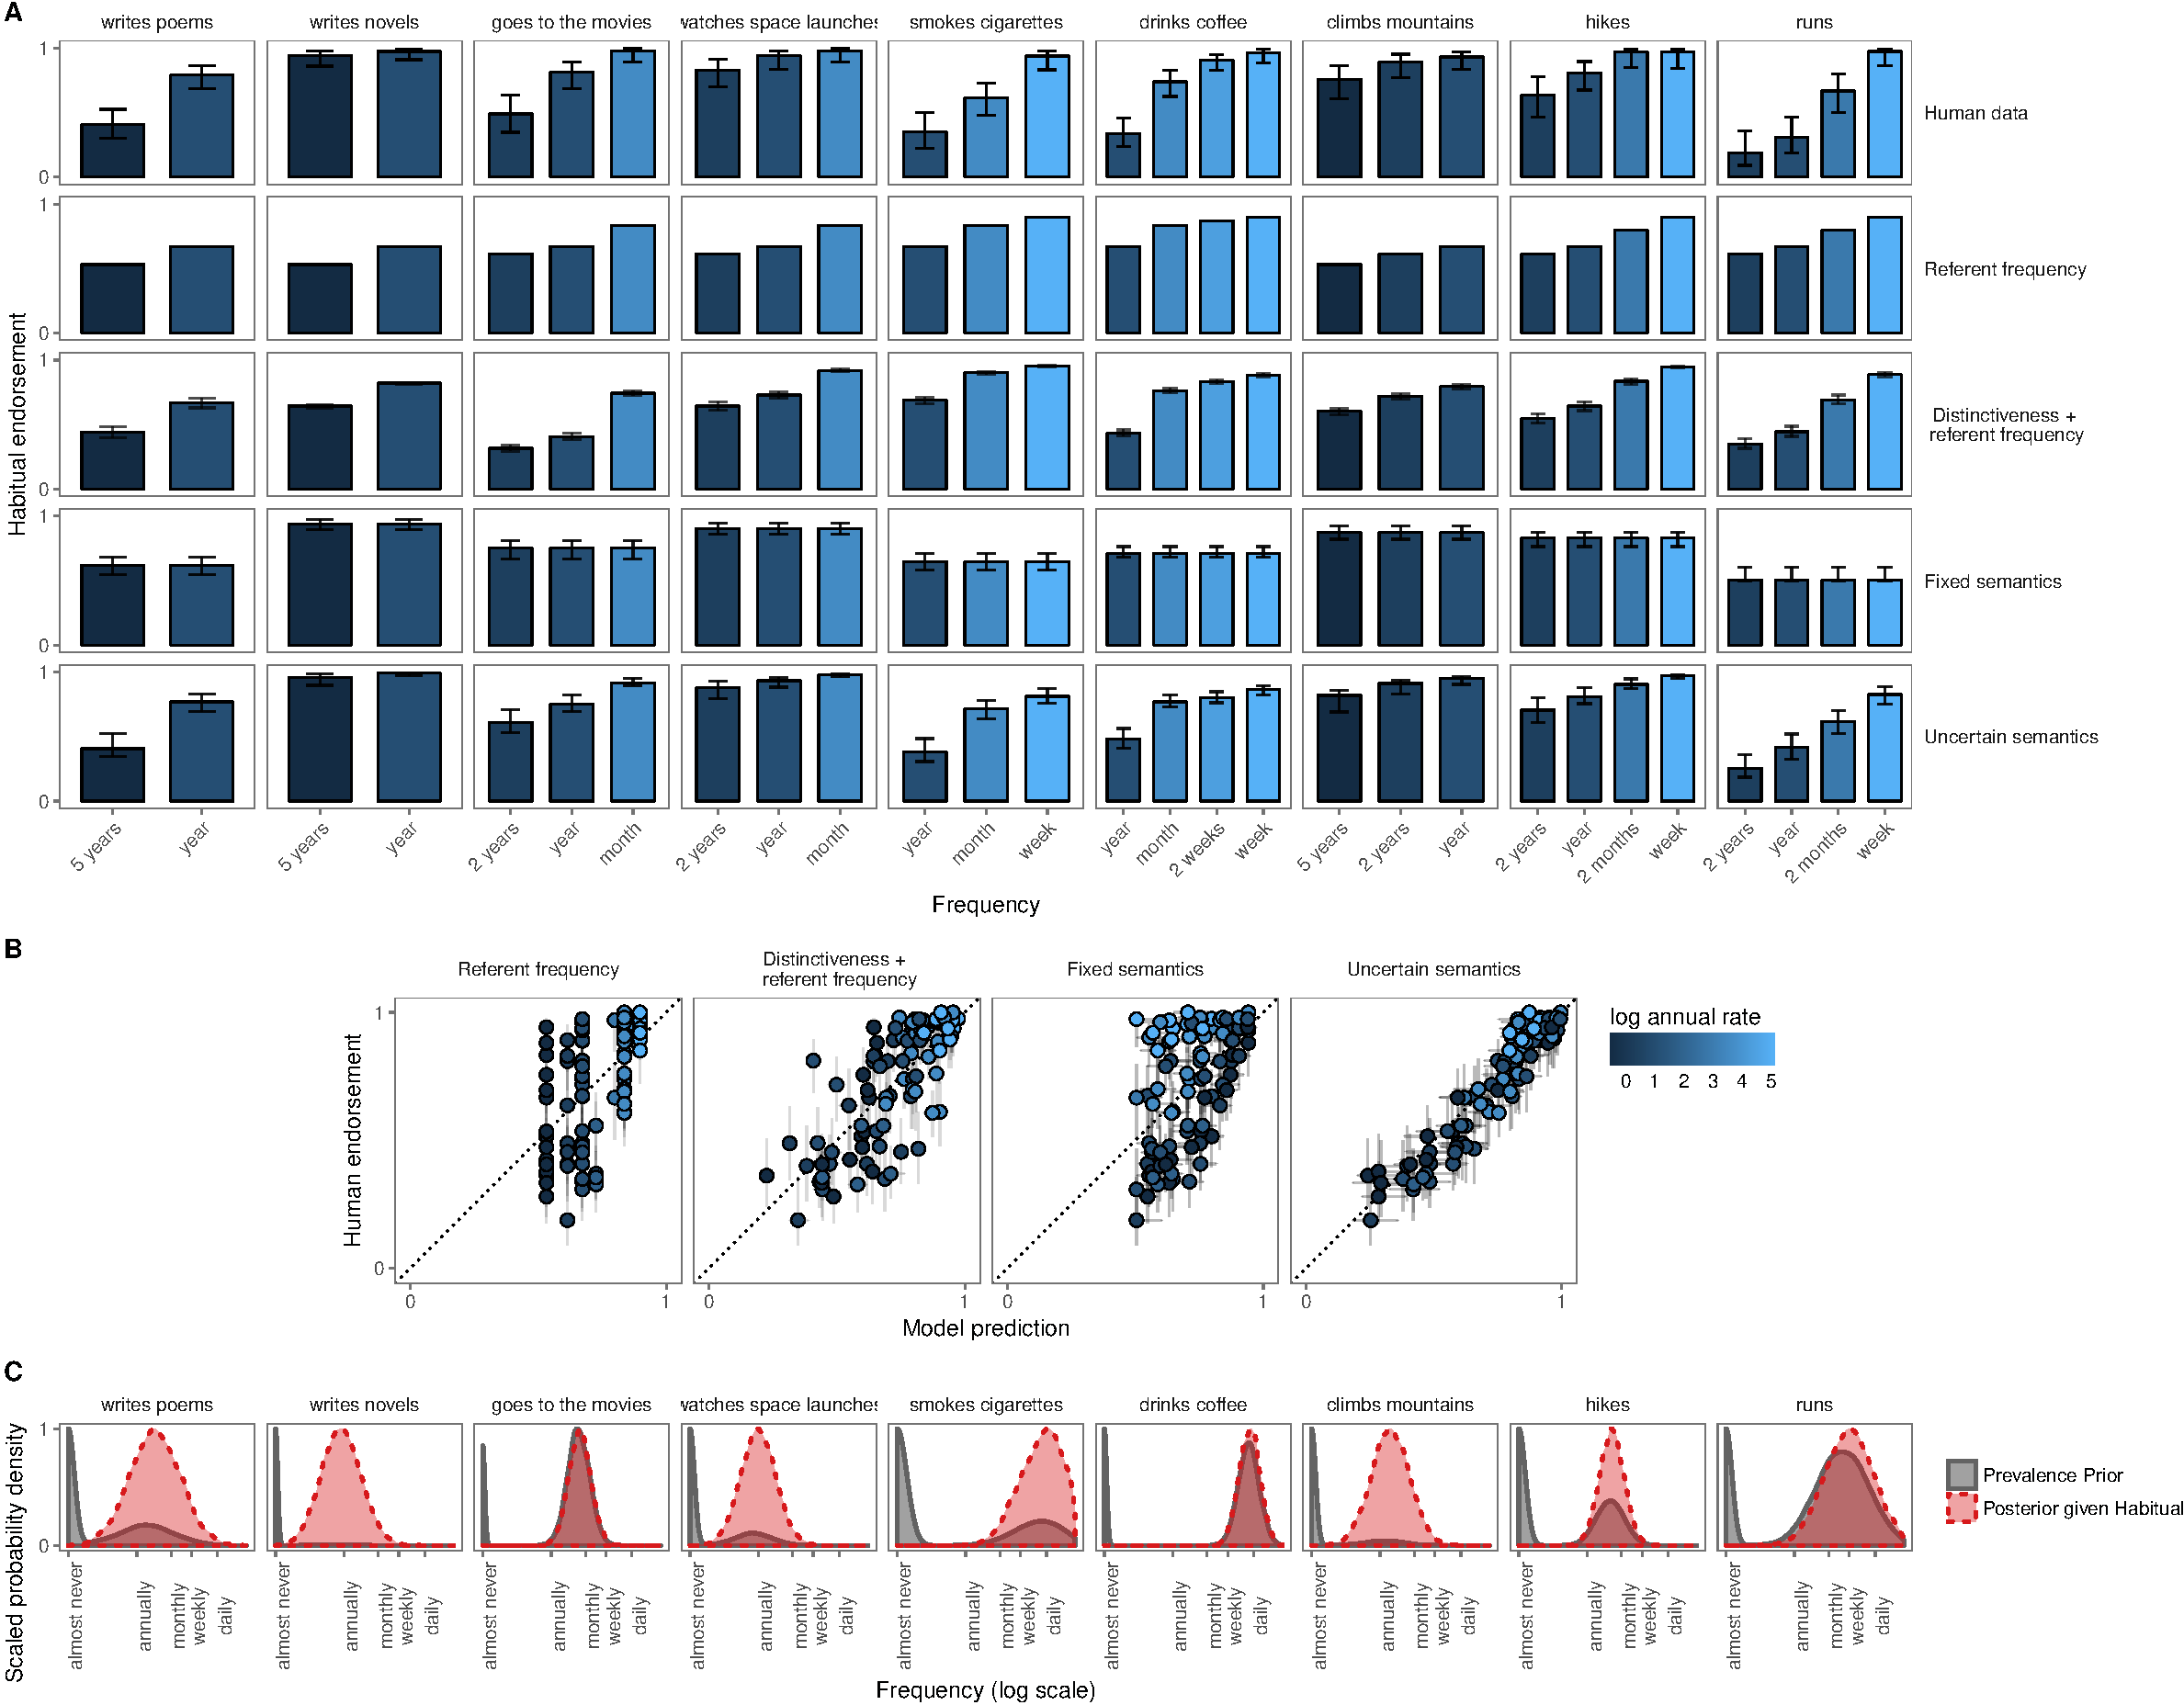
\includegraphics{figs/habituals-endorsement-figure-1.pdf}
\caption{\label{fig:habituals-endorsement-figure}Endorsing generalizations
about events. A: Endorsements for nine events given different
frequencies of action by human participants and four models. B: Human
elicited endorsements for ninety-three habitual sentences as a function
of the referent (log) frequency of action. Top right: Model fits for all
ninety-three habitual sentences by each model. C: Nine example frequency
priors and posteriors upon hearing the generalization. These
distributions are inferred using both data sources from Expts. 2a \&
2b.}
\end{figure}

In an exploratory analysis, we find no differences between endorsements
of the habitual of characters with male and female names, and overall,
the mean endorsements by gender are strongly correlated
\(r(93) = 0.91\). Endorsements are even more highly correlated for the
six events we anticipated differences by referent-gender:
\(r(21) = 0.97\) This lack of a difference may be because the felicity
of habitual sentences depends on a comparison to individuals of both
genders (i.e, in minimal contexts such as this, habituals are evaluated
with respect to \emph{other people}, not just other men or other women).
Less interestingly, the lack of a difference may be the result of gender
being not very salient in our paradigm, perhaps because the names used
were not sufficiently gendered.

We now turn to our model-based analyses to better understand the
endorsement data and the contribution of our model. For all analyses, we
collapse across gender of the referent character for endorsement
judgments. Parallel to our analysis of generic language endorsements, we
articulate a set of simple regression models and an alternative to our
uncertain-threshold endorsement model. Analyses which use the rate prior
distribution \(P(p_f)\) (all models except \enquote{referent frequency}
regression) use a 50\% mixture of the inferred priors for each gender to
construct a single prior distribution. To model the uncertainty in the
input measurements, we bootstrap the data for the regression models and
we construct joint-inference, Bayesian data analytic models for the
information-theoretic endorsement models (fixed-threshold and
uncertain-thresold).

\paragraph{Referent frequency}\label{referent-frequency}

To understand the role of frequency in habitual endorsement, we use the
frequency supplied to the participants in our experiment as a predictor
in a linear model. This model predicts the same endorsement level for
two actions done with the same rate. Obvious counterexamples exist in
our data set: While participants are willing to endorse that a person
\enquote{\ldots{} climbs mountains} having done it 3 times in the past
\emph{year}, they are less willing to say that a person
\enquote{\ldots{} hikes} and not willing to say that a person
\enquote{\ldots{} runs}. Some actions done with a relative high rate
(e.g., 3 times in a month) do not receive full endorsement (e.g.,
\emph{smokes cigarettes}; Figure \ref{fig:habituals-endorsement-figure}
A). Overall, the referent-frequency (in log-scale) predicts only a
fraction of the variability in responses (\(r^2(93) = 0.325\);
MSE=\(0.0355\)). In addition, for actions that are done on the time
scale of years or longer (lower median of frequency), referent frequency
no longer explains endorsements (\(r^2(50) = 0.0662\); MSE =\(0.0477\)).
The prevalence baseline does appreciably worse in this data set in
comparison to the generics data set (Case Study 1) because we designed
the stimulus set to be critical of a referent-frequency model.

\paragraph{Distinctiveness and referent
frequency}\label{distinctiveness-and-referent-frequency}

In our empirically elicited priors, items differ the proportion of
people who have done the action before (the \emph{mixture parameter} of
the mixture model; Figure \ref{fig:habituals-prior-figure}). This
mixture parameter is a major contributor to the mean of the prevalence
prior distribution, and thus is relates to the \emph{cue validity} of a
particular feature for a particular individual (see Appendix A for a
derivation of the relationship between the prevalence prior and cue
validity). Thus, we take this parameter as an index of the
\emph{distinctiveness} of the action, analagous to \emph{cue validity}
in the case study of generic langauge. We construct a regression model
that treats endorsement as a linear combination of frequency and
distinctiveness information. We use participants' responses to the
question about the mixture parameter \(\phi\) (i.e., the proportion of
people who have done the action before) as well as frequency given to
participants to predict habitual endorsement.

This model is able to explain more of the variance in endorsements
(\(r^2(93) = 0.583\); MSE=\(0.0219\)). It can differentiate events done
with the same frequency (e.g., \emph{writing poems} vs. \emph{novels}, 3
times in the past 5 years), and increase endorsement of the more rare
action (\emph{novels}). Still, this model fails to capture fine-grained
details in endorsment. For example, going to the movies is a relatively
nondistinctive action (many people do it) and going three times in a
year is not very frequent, and yet people still strongly endorse the
habitual \(0.81 [0.69, 0.89]\), while this regression model predicts
quite lower judgments \(0.41 [0.38, 0.43]\). On the other hand, playing
the banjo three times in the past two years is not strong evidence for
the habitual, according to participants \(0.45 [0.33, 0.59]\).
Nevertheless, because playing the banjo is a distinct skill, the
regression model wants to endorse the habitual strongly in this case
\(0.75 [0.74, 0.76]\).

\paragraph{Fixed-threshold endorsement
model}\label{fixed-threshold-endorsement-model}

We next examine an information-theoretic endorsement model based on a
fixed-threshold semantics. A fixed-threshold model commits the habitual
to conveying that a person \emph{does the action with some rate}, and
the threshold on rates is common to all actions. As in Case Study 1, we
incorporate this model into a Bayesian joint-inference model to infer
the fixed-threshold and simultaneously predict both the priors data and
the endorsement data (for more details on model implementation, see
Appendix C). We assume the referent-prevalence \(p_{fk}\) being conveyed
by the endorsement model (Eq. \ref{eq:S1}) is the frequency provided to
participants (e.g., 3 times in the past year). Additionally, to account
for statements that would be literally false under this model
(frequencies that fall below the fixed threshold), we include an
additional noise parameter, as we did for the fixed-threshold model in
Case Study 1. To learn about the credible values of the model's
parameters and generate predictions given those inferred parameter
values, we collected 2 MCMC chains of 100,000 iterations, discarding the
first 50,000 iterations for burn in.

The data analytic model infers that a low threshold is likely: the
inferred threshold in units of number of times per year is 0.01 {[}0.01,
0.37{]}. Compare this with the lowest referent-frequency used in our
data set: \(0.6\) times per year (3 times every 5 years). Thus, all of
the utterances evaluated under this fixed-threshold model were literally
true. As a result, the lowest endorsement this model can apply to an
utterance is 0.5 (since both the habitual and silence are always true).
The fixed-threshold model exhibits a small dynamic range of
endorsements, similar to the referent-frequency model.

A fixed-threshold utterance updates the interpreter model's beliefs
differentially depending on the item. For instance, it's highly unlikely
that a random person \emph{climbs mountains} with any non-zero rate;
thus this model fully endorses \enquote{Mary climbs mountains} even with
low-frequency (Figure \ref{fig:habituals-endorsement-figure} A).
However, the model doesn't differentiate doing the same action with
different frequencies. It is equally true that a person does an action
\emph{with some frequency} for any frequency greater than zero,
analogous to how \enquote{some Ks F} is equally true if 20\% or 50\% of
Ks F.

Finally, the data-analytic model infers that 10\% {[}1, 19{]} of the
data is noise and that the speaker optimality parameter is 0.77 {[}0.70,
1.25{]}.

\paragraph{Uncertain-threshold endorsement
model}\label{uncertain-threshold-endorsement-model}

We used the same data analytic approach for the uncertain threshold
endorsement model and performed the same Bayesian statistical inference
over the model to learn about its parameters and predictions. Again,
this model has two fewer parameters than the fixed-threshold model (no
fixed-threshold parameter and no extrinsic noise process). As shown in
Figure \ref{fig:habituals-endorsement-figure}B, the uncertain-threshold
endorsement model does a good job of accounting for the variability in
responses (\(r^2(93) = 0.894\); MSE=\(0.00598\)), including actions done
on the time scale of years or more (\(r^2(50) = 0.903\);
MSE=\(0.00617\)). Figure \ref{fig:habituals-endorsement-figure}C
provides insight into how the model achieves this. An interpreter who
hears a generalization interprets it relative the prior distribution
over frequencies, which results in different points at which the
generalization is good statement to assert. Someone who smoked
cigarettes 3 times last month is not fully someone who \enquote{smokes
cigarettes}, whereas someone who went to the movies 3 times last month
more a person who \enquote{goes to the movies}. Only the
uncertain-threshold model is able to draw this fine distinction.

\subsubsection{Discussion}\label{discussion-1}

Habitual language exhibits context-sensitivity directly parallel to that
of generic language (Case Study 1). Habituals are endorsed for a wide
range of frequencies, but show systematic patterns relative to the prior
distribution of frequencies, as formalized by the uncertain-threshold
model. Again, we articulated a number of alternative models and found
that only the underspecified threshold model was able to explain the
variability in endorsements.

In this case study, we manipulated rather than measured the referent
frequency (e.g., the frequency with which a person drinks coffee). By
manipulating the target frequency, we have shown that it is causally
related to habitual endorsements in the way predicted by our model (and
in a way that a fixed-threshold model cannot account for). The
relationship is not linear (or log-linear), however; habitual
endorsements vary in complex ways that reflect interpreters' prior
knowledge about the event in question.

In Expt. 2b, participants were given a statement about how often a
person has done the action in the past and asked to judge the
corresponding habitual statement. This design potentially confounds an
important distinction for the language of generalization: Does the
prevalence communicated by a generalization indicate an objective, past
frequency or a subjective, future expectation? In Expt. 2c, we
investigate this question by teasing apart \emph{past} from
\emph{predictive frequency} and measuring its influence on habitual
endorsement.

\subsection{Experiment 2c: What is
prevalence?}\label{experiment-2c-what-is-prevalence}

While past frequency is often a good indicator of future tendency, the
future is under no obligation to mimic the past. Does habitual language
communicate probabilities in terms of past frequency or future
expectations? On one hand, speakers can only be certain about what has
happened in the past. On the other hand, language has a communicative
function, and it would be useful for speakers to convey their
predictions of what will be the case in the future.

People can change their behavior abruptly due to a variety of decisions
and outside events. We introduce these causal events into our minimal
endorsement paradigm and measure their influence on endorsement. To
provide the appropriate model-based analysis, participants in one
condition make a prediction about what will be the case in the future
(\emph{predictive frequency}). In another condition, participants decide
whether or not to endorse the habitual sentence (as in Expt. 2b). We
then compare two uncertain-thresholds models to each other: one which
uses participants' ratings of \emph{predictive frequency} as the object
of communication and one which uses the \emph{past frequency} (as was
done for Expt. 2b).

\begin{figure}[htbp]
\centering
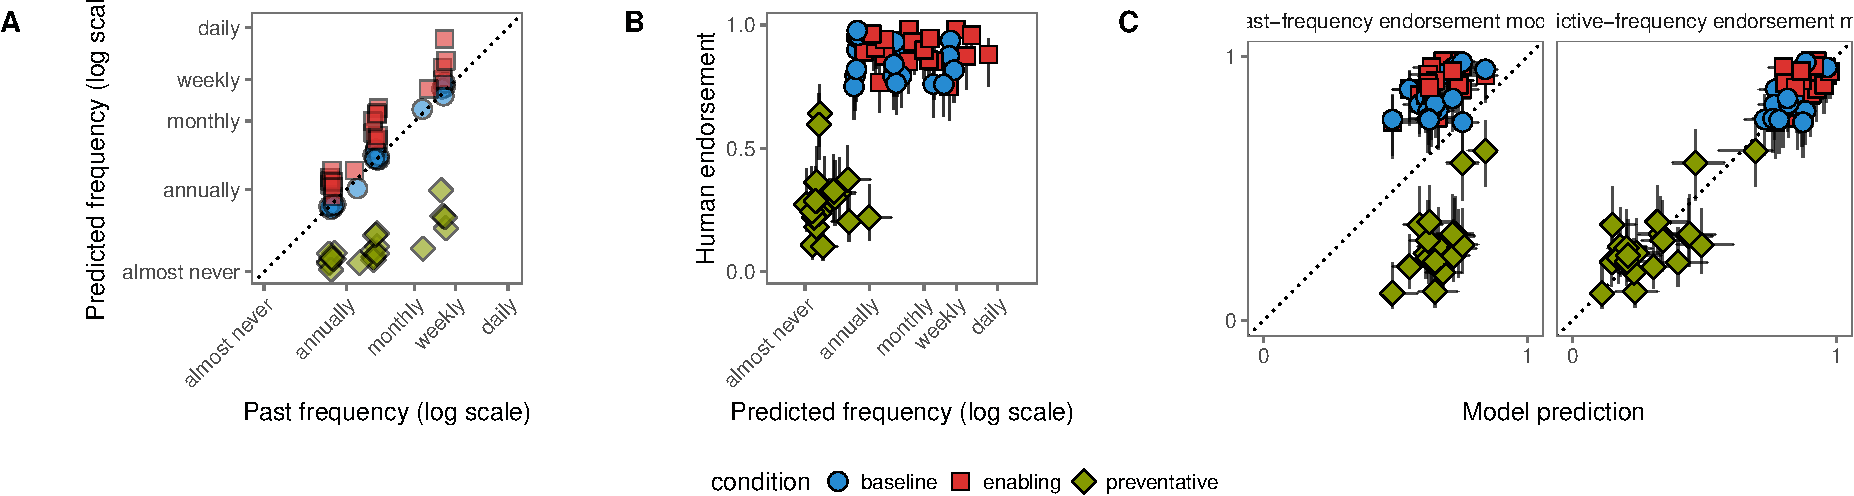
\includegraphics{figs/habituals-predictive-figure-1.pdf}
\caption{\label{fig:habituals-predictive-figure}Top left: Predicted
frequency of event (log-scale) as a function of (log) past frequency and
condition manipulation (enabling, preventative, and baseline). Top
right: Human endorsement of habitual sentences as a function of log
predicted frequency and condition manipulation. Bottom row: Endorsement
models based on past frequency (left) and measured predictive frequency
(row).}
\end{figure}

\subsubsection{Method}\label{method-4}

\paragraph{Participants}\label{participants-4}

We recruited 270 participants from MTurk, using the same criterion as
Expt. 2b. 120 were assigned to the \emph{predictive frequency} condition
and 150 were assigned to the \emph{sentence endorsement} condition. The
experiment took on average minutes (\emph{predictive frequency}) and
minutes (\emph{sentence endorsement}). Participants were compensated
\$0.40.

\paragraph{Materials}\label{materials-2}

The events used were a subset of those used in Expts. 2a \& b (21 of the
original 31). In addition, we crafted statements that were intended to
either increase the frequency (\emph{enabling}; e.g.,
\enquote{Yesterday, Bill bought a pack of cigarettes.}) or decrease the
frequency (\emph{preventative}; \enquote{Yesterday, Bill quit smoking.})
of the event in the future. In order to increase the potential
variability of responses across the experimental conditions,
participants only saw the frequencies that led to the most intermediate
endorsement of the habitual in Expt. 2b. We did not include separate
trials for both male and female names for the select items we did in
Expt. 2b, since we saw no differences in their endorsements of the
habitual. See Appendix D for a full list of the enabling and
preventative information.

\paragraph{Procedure}\label{procedure-2}

The procedure was identical to Expt. 2b except for the inclusion of a
second sentence on a subset of trials (\emph{preventative} and
\emph{enabling} trials). On all trials, participants were presented with
a \emph{past frequency sentence} (same as Expt. 2b). Additionally,
trials either included \emph{preventative} information, \emph{enabling}
information, or no additional information (identical to Expt. 2b), in
equal proportions.

In the \emph{predictive frequency} condition, participants were asked
``In the next \textsc{time window}, how many times do you think
\textsc{person} does \textsc{action}?'', where the \textsc{time window}
was the same as given in the \emph{past frequency statement}. In the
\emph{sentence endorsement} condition, participants were asked if they
agreed or disagreed with the corresponding habitual sentence (as in
Expt. 2b).

\subsubsection{Results}\label{results-3}

\paragraph{Predictive frequency}\label{predictive-frequency}

Figure \ref{fig:habituals-predictive-figure} (left) shows the mean
predicted future rate as a function of the past rate given to the
participant and the type of causal information given. We observe in the
baseline condition that future frequency perfectly tracks past frequency
(\(r(21) = 0.99\)). That is, participants believe if a person smoked
cigarettes 3 times last month, they will smoke cigarettes 3 times next
month. This result implies that our model makes identical predictions
for Expt. 2b whether the referent is past frequency or expected future
frequency (indicating, as expected, that we must look to the new data to
distinguish these models). Critically, we observe the preventative
information strongly decreases and the enabling information slightly
increases predicted frequency (Figure
\ref{fig:habituals-predictive-elicitation} left; blue and green dots).

We confirm these observations using a linear mixed-effects model,
predicting the log-transformed responses from the log-transormed past
frequency and the experimental condition (baseline, preventative,
enabling). To account for participant and item variability in this
analysis, we also include random effects of intercept and condition for
both participants and items. Confirming our predictions, the
preventative information led to significantly lower predictions for
future frequency, relative to the baseline condition (
\(\beta = -3.18\); \(SE = 0.27;\) \(t = -11.96\) ). There was also
tendency for the enabling information to lead to higher predictions for
future frequency, relative to baseline ( \(\beta = 0.96\);
\(SE = 0.11;\) \(t = 8.54\) ). Finally, past frequency was a significant
predictor of predicted future frequency ( \(\beta = 1.01\);
\(SE = 0.02;\) \(t = 40.80\) ).

\paragraph{Sentence endorsement}\label{sentence-endorsement}

There is a clear and consistent negative effect of preventative
information on endorsements for the habitual sentence (Figure
\ref{fig:habituals-predictive-figure}B; green points). Still, frequency
--- even predictive frequency --- does not perfectly explain the
endorsements (\(r^2(63) = 0.518\); MSE = \(4.3\)). When collapsing
across items, the Bayesian Maximum A-Posteriori estimate and 95\%
highest probability density interval for the true endorsement
probabilities per condition are: baseline = 0.85 {[}0.83, 0.87{]},
enabling = 0.90 {[}0.88, 0.92{]}, preventative = 0.29 {[}0.26, 0.32{]}

We use our formal model to test whether past or predictive frequency
matters for endorsement. To formalize the predictive frequency speaker
model, we use the mean predictive frequency as the referent-prevalence
\(p_{fk}\) that the endorsement model (Eq. \ref{eq:S1}) conditions on.
The past frequency model is constructed using the past frequency
supplied to participants as the referent-prevalence. We analyze this
model in the same Bayesian data analysis regime as for our previous
models. We use the same priors over the parameters as before and learn
about the posterior distribution by collecting three independent MCMC
chains of 100,000 iterations (removing the first 50,000 for burn-in).
Figure \ref{fig:habituals-predictive-figure}C shows the resulting model
predictions for the past frequency and the predictive frequency
endorsement models. Participants' judgments of the habitual statements
was indeed influenced by the causal manipulations \emph{in the way
predicted} by the endorsement model that uses the predictive frequency
as the object of communication (\(r^2(63) = 0.931\); MSE = \(0.00594\)).
The model based on past frequency does not make different predictions
for the different causal manipulation conditions and does a poor job at
explaining the endorsements (\(r^2(63) = 0.0334\); MSE = \(0.0833\)).

\subsection{Discussion}\label{discussion-2}

Habitual language conveys generalizations about events. Our model
decides if a habitual sentence is a pragmatically useful way to describe
the rate at which a person does an action, taking into account a naive
interpreter's prior beliefs about the event (measured in Expt. 2a). Our
computational model endorses statements that communicate generalizations
about events with the same sensitivity to context and frequency that
people exhibit (Expt. 2b \& c). In Expt. 2b, we varied the type of event
and the past frequency with which the person did the action, and found
graded endorsements of the corresponding habitual sentences. By
manipulating (rather than measuring) the referent frequency with which a
person does an action, we showed how alternative models were
insufficient to account for the gradience in endorsement. In particular,
a fixed threshold model that has access to the same prior knowledge and
uses the same information-theoretic decision rule as our
uncertain-threshold model is unable to make different predictions for
different frequencies. Only our uncertain threshold model was able to
precisely account for the wide range of endorsements.

A regression model that takes into the frequency and the
\emph{distinctiveness} of the action does a reasonable job at explaining
the variance in this data. We note that this kind of model is merely a
re-decription of the data (and thus, the behavior of the uncertain
threshold model), and does not represent a theory of the semantics of a
generalization. A theory of the semantics of a generalization must
formalize the truth-conditions of the generalization as well as how
those truth-conditions relate to endorsement. This is precisely what our
information-theoretic models do (both fixed- and uncertain-threshold).

In Expt. 2c, we further investigated the nature of the underlying
prevalence scale by introducing causal information that enabled and
preventated future occurences of the action. We used the
empirically-measured predicted future frequency as the object of
communication for our endorsement model. We found that the endorsement
model that seeks to communicate its predictions (rather than its
observations) is a better model of habitual endorsements under these
situations. Predicted prevalence thus captures the infleunce of top-down
moderators (e.g., intervening causal forces) on endorsement.

In these experiments, we introduced participants to novel actors and, by
doing so, were able to directly manipulate the frequency of a person
doing the action. The kinds of events we used were familiar to
participants (e.g., \emph{running}) and thus we measured the prevalence
priors for those events. In our final case study, we experimentally
manipulate the prevalence priors, testing their causal influence over
endorsements. In addition, we further we extend our theory to the
language of causal relationships.

\section{Case Study 3: Causal
Language}\label{case-study-3-causal-language}

Language about causal relationships manifests in generalization. The
utterance \enquote{Drinking moonshine makes you go blind} relates to
\enquote{My grandpa's drinking moonshine made him go blind} in a way
analagous to how \enquote{John smokes} relates to \enquote{John smoked
yesterday}. We explore this hypothesis in our third case study: causal
language or \emph{causals} (e.g., \enquote{A causes B}).

The problem of \emph{causal induction}---knowing that one thing causes
another----has been studied extensively in human psychology (Cheng,
1997; Cheng \& Npvick, 1992; Griffiths \& Tenenbaum, 2005, 2009).
Classically, this is cast as a problem of inducing an unobservable
relation (\emph{type causation}) from observable events or contingency
data. We take a different approaching, examining \emph{type causation}
by the language used to describe it (e.g., \enquote{A causes B}). We
explore the idea that such language conveys a generalization about \emph{token} or
\emph{actual causation} (e.g., \enquote{A caused B, in this instance})
and that our theory of the language of generalizations extends in a
natural way to describe \emph{causal language}. Ascribing causation to
an individual event (\emph{token or actual causation}) is itself a
complex, inferential process (e.g., depending on counterfactual
reasoning; T. Gerstenberg, Goodman, Lagnado, \& Tenenbaum, 2015), which
we do not try to model here.

In this paper, we posit thatprevalence priors are a mediating
representation between abstract conceptual structure and generalizations
in language. In this last set of experiments, we explicitly test the
relationship between the prevalence priors and endorsements of
generalizations about causes. Also, by designing the experiments in the
domain of causal language, we further demonstrate the generality of our
theory of communicating generalizations.

\subsection{Experiment 3a: Manipulating prevalence
priors}\label{experiment-3a-manipulating-prevalence-priors}

In this experiment, we manipulate and measure participants' background
knowledge in order to check whether or not manipulation of participants'
background knowledge was successful. Experiment 3b (\emph{causal
endorsement}) will then follow a mostly-identical experimental
procedure.

\subsubsection{Method}\label{method-5}

\paragraph{Participants}\label{participants-5}

We recruited 160 participants from Amazon's Mechanical Turk.
Participants were restricted to those with U.S. IP addresses and who had
at least a 95\% work approval rating. The experiment took on average
1.70 minutes and participants were compensated \$0.50 for their work.

\paragraph{Materials}\label{materials-3}

Participants were told a story of a scientific experiment testing
different substances to produce an effect (either to make animals sleepy
or plants grow tall). Our cover stories were constructed so that the
potential cause could have some plausible intuitive mechanism that could
give rise to the proprety (e.g., a naturally occurring herb causing
animals to be sleepy). The two cover stories can be seen in Table
\ref{tab:causalItems}.

Participants were then shown \enquote{previous experimental results},
which followed one of four distributions, shown in Figure
\ref{fig:causals-conditions}. In two of the conditions, participants saw
results that came from the same underlying distribution. In one of these
conditions, all causes produced a strong effect (average efficacy
approximately 98\%; the \enquote{common strong} condition). In the
second of these conditions, all causes produced a weak effect (average
efficacy approximately 20\%; the \enquote{common weak} condition). The
two other conditions used distributions in which some experiments
resulted in either no or very few succeses (i.e., produced 0s or 1s or
2s), and others that either had strong or weak effects as above. These
are the \enquote{rare strong} and \enquote{rare weak} conditions.

\begin{table}[]
\centering
\label{tab:causalMaterials}
\resizebox{\textwidth}{!}{
\begin{tabular}{|p{3cm}|p{6.5cm}|p{6.5cm}|}
\hline
                   & Plants                                                                                                                                                                                                  & Animals                                                                                                                                                                                                                               \\ \hline
Cover story        & On this planet, there is a plant called feps and your team wants to figure out how to make these plants grow tall. Your team runs experiments trying to make feps grow tall with different fertilizers. & On this planet, there are animals called cheebas and your team of scientists wants to figure out how to make these animals sleepy. Your team runs experiments trying to make cheebas sleepy with different naturally occurring herbs. \\ \hline
Evidence statement & Your team gave fertilizer B to 100 different feps. Of those 100 treated, 2 feps grew tall.                                                                                                              & Your team gave herb C to 100 different cheebas. Of those 100 treated, 98 cheebas were made sleepy.    \\   \hline                                                                                                                            
\end{tabular}
}
\caption{Cover stories and evidence statements for the two sets of materials used in Expt. 3a\&b}
\end{table}

\begin{figure}[htbp]
\centering
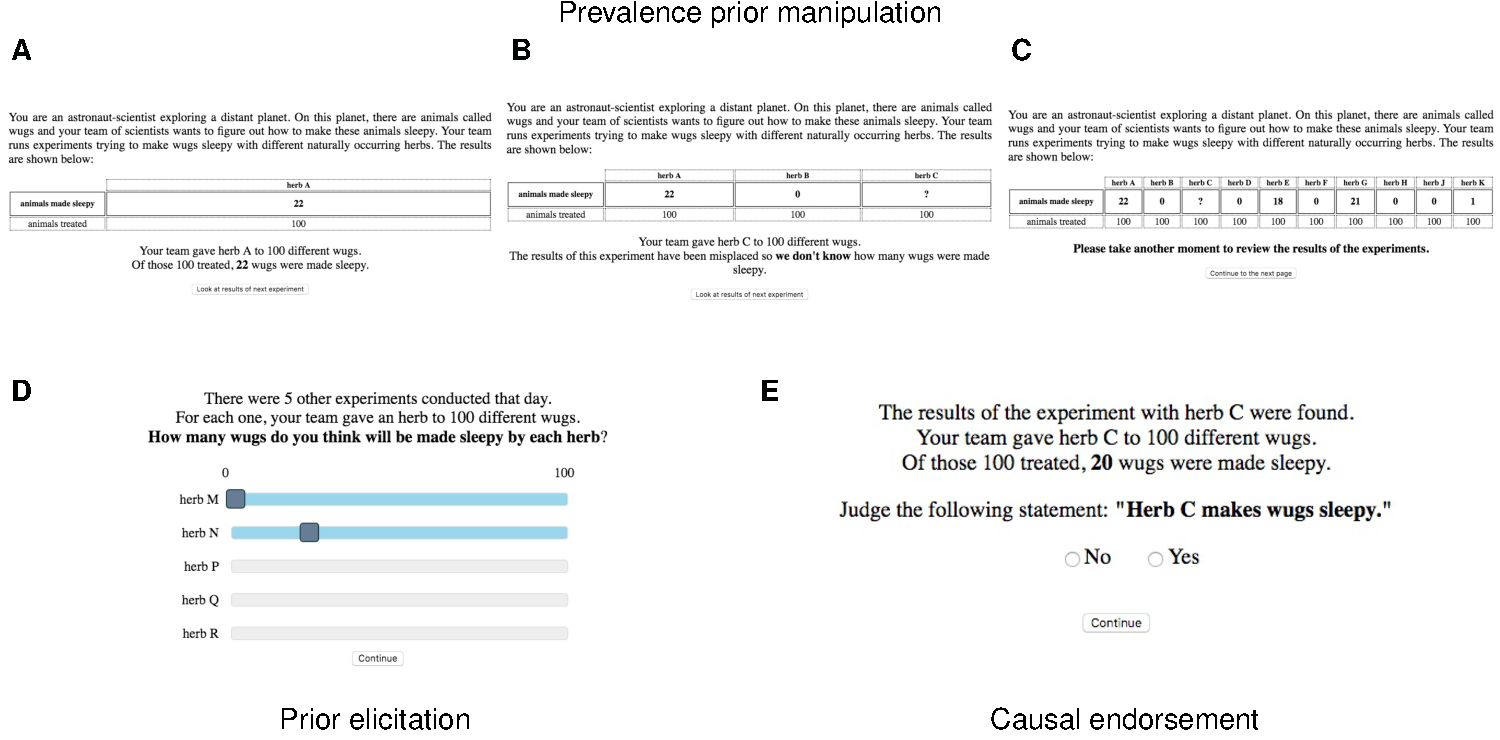
\includegraphics{figs/causalExpt-1.pdf}
\caption{\label{fig:causalExpt}Overview of Experiment 3. A-C: Results of
previous experiments are shown one at a time, described in text and
displayed in a table. One of the results was lost. Participants are
asked to review previous results once all displayed. B: Prior
elicitation task: Participants predict the results of the next 5
experiments. D: Causal endorsement task: Results of previously lost
experiment are found and participants are asked to evaluate the causal
generalization.}
\end{figure}

\paragraph{Procedure}\label{procedure-3}

Each participant saw only one cover story with one distribution of
previous experiments (i.e., the experiment was a single trial).
Participants were told that they were an astronaut-scientist on a
distant planet trying to figure out how some system works (i.e., how to
make a certain kind of animal sleepy with different herbs or how to make
a plant grow tall with different fertilizers). The story for the
\enquote{sleepy animals} condition read:

\begin{quotation}
You are an astronaut-scientist exploring a distant planet. 
On this planet, there are animals called cheebas and your team of scientists wants to figure out how to make these animals sleepy.
Your team runs experiments trying to make cheebas sleepy with different naturally occurring herbs.
The results are shown below:
\end{quotation}

Participants then click a button to show the results of the experiments.
Experiment results appear one at a time (upon a click), and are
described in an \emph{evidence statement} (e.g., \enquote{Your team gave
herb A to 100 different cheebas. Of those 100 treated, 98 cheebas were
made sleepy.}) as well as displayed in a table showing the number of
successes (e.g., \enquote{animals made sleepy}) per number of attempts
(always 100 per experiment). We described the results of these
individual experiments using \emph{token-level} causal language (e.g.,
\enquote{98 cheebas were made sleepy}) to suggest that actual causation
occurred in these cases.

Participants see the results of eleven \enquote{experiments}, though
they are told the results of one experiment were lost and a \enquote{?}
was placed in the table (Figure \ref{fig:causalExpt}). (These lost
results would be found in the \emph{causal endorsement} task, Expt. 3b).
After participants viewed the results of the 10 \enquote{experiments}
(and 1 missing experiment), they are told to review the results of the
experiments before continuing.

Upon clicking the continue button, the table of experiment results is
removed and participants are told more experiments were conducted.
Participants were asked to predict the results of the next 5
experiments. Participants were given 5 slider bars ranging from 0 - 100,
and asked to predict the next five substances (e.g., herbs M, N, P, Q,
and R).

After responding, participants then completed an attention check survey
where they were asked what the team of scientists were investigated
(choosing a response from a drop-down menu with 12 options) and to input
one of the numerical results they saw on the previous screen. This
attention check served to confirm that participants had encoded some
part of both relevant aspects of the experiment (the domain and the
frequencies).

\subsubsection{Results}\label{results-4}

20 participants were excluded from the analysis for failing to answer
both of the attention check questions correctly, leaving a total of 140
responses for analysis. The distributions that resulted from
participants predicting the causal efficacy of the new substances are
shown in Figure \ref{fig:figure-causals}. These distributions nicely
recapitulate the distributions supplied in the different experimental
conditions, suggesting that the manipulation does indeed change
participants' representations of what probabilities are likely to occur
in each experimental condition. We hypothesize that with the
distributions altered, endorsements of generalizations will similarly be
affected.

\subsection{Experiment 3b: Causal
Endorsements}\label{experiment-3b-causal-endorsements}

In this experiment, we tested whether the manipulated priors of Expt. 3a
are causally related to the endorsement of causal statements. Most of
the experimental deisgn was identical to that of Experiment 3a.

\subsubsection{Method}\label{method-6}

\paragraph{Participants}\label{participants-6}

We recruited 400 participants from Amazon's Mechanical Turk.
Participants were restricted to those with U.S. IP addresses and who had
at least a 95\% work approval rating. None of the participants had
participated in Experiment 3a. The experiment consisted of one trial and
took on average 1.40 minutes; participants were compensated \$0.25 for
their work.

\paragraph{Procedure and materials}\label{procedure-and-materials-2}

The materials were the same as in Experiment 3a, The first part of the
experimental trial was the same as in Expt. 3a (the table of
\enquote{previous experiments}; Figure \ref{fig:causalExpt}). Upon
continuing beyond the first part of the trial, the table of results and
background story were removed from the screen and the participant is
told that the results of the \enquote{lost experiment} were found. The
results are reported to the participant in terms of how many out of 100
of the attempts were successful. Participants saw 1 of 2 reported
frequencies: 20\% or 70\% (randomized between-subjects). Participants
were then asked to judge the causal sentence (e.g., \enquote{Herb X
makes the animals sleepy}). Partipants responded by either clicking
\enquote{Yes} or \enquote{No}. After responding, participants completed
the same attention check as Expt. 3a.

\begin{figure}[htbp]
\centering
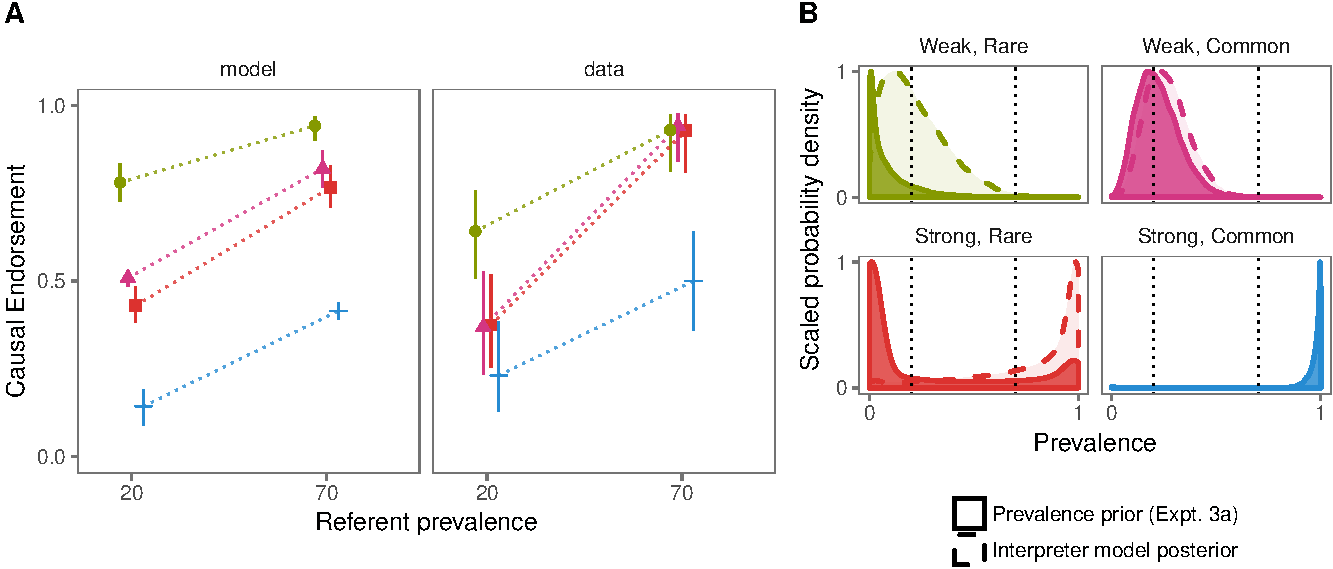
\includegraphics{figs/figure-causals-1.pdf}
\caption{\label{fig:figure-causals}Endorsing generalizations about causes.
A: Endorsement model predictions (left) and human elicited endorsements
(right) for four background distributions and two observed frequencies.
B: Prevalence prior distributions and interpreter model posteriors upon
hearing a causal generalization, for the experimentally manipulated
priors. Vertical lines denote referent-prevalence levels for the causal
endorsement task. Endorsement mode predictions, interpreter model
posteriors, and prevalence priors are inferred using both Expt. 3a and
3b data, following the same Bayesian data analytic approach outlined in
Appendix C.}
\end{figure}

\subsubsection{Results}\label{results-5}

42 participants were excluded from the analysis for failing to answer
both of the attention check questions correctly, leaving a total of 358
responses for analysis. As in our other analyses of endorsement
responses, we computed the Bayesian Maximum A-Posteriori (MAP) estimate
and 95\% highest probability density interval of the true population
probability of endorsing the statement, assuming a uniform prior. These
are shown for the different experimentally-manipulated priors and
frequencies in Figure \ref{fig:causals-endorsement}.

As predicted by our model, endorsements for a causal statement were
sensitive to the background distribution of other causes and the causal
power of the target cause. When many other causes produced the effect
very reliably (\emph{common deterministic} condition), very few
participants endorsed the causal statement for a cause with causal power
of 0.2, and were at chance when the causal power was 0.7 (Figure
\textbackslash{}ref\{fig:figure-causals-endorsement; top, blue). By
contrast, when many other causes failed to produce the effect and those
that did were not very reliable (\emph{rare weak} condition; green in
figure), at least half of participants endorsed the causal statement for
a cause with causal power of 0.2, and were at ceiling when the causal
power was 0.7. The other two conditions (\emph{rare deterministic} and
\emph{common weak}) led to endorsements intermediate between these two
conditions. Our model predicted these effects again with strong
quantitative accuracy (\(r^2(8) = 0.835\); MSE = \(0.0123\)).

\subsection{Discussion}\label{discussion-3}

In our third case study, we applied our same model to generalizations
about causal events. In this domain, we succesfully manipulated
participants' beliefs about the expected prevalence of a causal
relationship in a domain (Expt. 3a). This was done using both unimodal
(\emph{common weak}, \emph{common strong}) and bimodal (\emph{rare
weak}, \emph{rare strong}) distributions. In Expt. 3b, we showed that
these manipulated priors influenced endorsements of the corresponding
causal statements. In addition to further demonstrating the generality
of this theory, these experiments show that the \emph{prevalence prior}
\(P(h)\) is causally related to endorsements of generalizations in
language. To our knowledge, these are the first experiments to
demonstrate how the probabilities of other categories having a feature
can influence endorsing a generalization about a different category.

In these experiments, we used two cover stories that described plausible
causal events: herbs making animals sleepy and fertilizers making plants
grow tall. We chose these items because there was a plausible causal
mechanism that could give rise to the property and these causal events
could have ambiguous causal power associated with them (e.g., it's
plausible that there are herbs that only weakly make animals sleepy and
it's also plausible that there are herbs that almost deterministically
make animals sleepy). These two features of the domains make them
particularly amenable to manipulation. That is, people's abstract
theories about these domains are flexible enough to permit such
manipulations.

It's likely that other domain knowledge would interact with the
experimentally-supplied \enquote{experimental data} to form a hybrid
belief distribution.\footnote{If this were happening in our domains, we
  would expect this to show up in the results of Expt. 3a. Participants'
  predictions about the likely causal power of new causes would be
  expected to show a mixture of their abstract, intuitive theories and
  the experimentally supplied data.} For example, physical causal
systems (e.g., billiard balls hitting each other) could strongly induce
near-deterministic notions of causal power, analagous to our
\enquote{deterministic} priors conditions. Causal systems that
demonstrate surprising or \emph{a priori} unlikely effects (e.g.,
liquids melting concrete) could induce rarity about the existence of a
non-zero causal power, analgous to our \enquote{rare} prior conditions.
Our theory would predict in these cases that differences in endorsement
would be attributable to differences in the prevalence prior
distribution (here: the belief distribution over causal power).

\section{General Discussion}\label{general-discussion}

It is a remarkable fact that so much is learned from ideas expressed
vaguely in words. Generalizations in language (e.g., \enquote{John
runs.}, \enquote{Dogs are friendly.}, \enquote{Staring at the sun makes
you go blind.}) are a premier example of how simple
statements---statements understood by even the youngest language
users---can display complex sensitivities to context. We have argued
that the core meaning of such linguistic expressions is, in fact,
simple, but underspecified. To our knowledge, this is the first formal
theory of generalizations in language that makes precise quantitative
predictions about human behavioral data.

As a formal theory of generalizations in language, we aim to unify
significant swaths of language that are, on their surface, quite
different from one another: generalizations about categories, events,
and causes. We have been able to formalize a unified, core meaning using
the underlying scale of \emph{prevalence}. We showed that all three
kinds of generalizations exhibit the same kind of sensitivity to context
(Expt. 1, 2a \& 2b, 3). Our framework naturally accounts for a number of
classic examples from the semantics of \emph{generic language} (Expt.
1). We provide an avenue for top-down moderators on language use, by
elucidating the scale as defined by a subjective, predictive
probability, not mere frequency (Expts. 2c \& 2d). Finally, we have
shown that listeners' prior knowledge about the prevalence of the
feature in a category is causally related to their endorsement of
statements of genericity (Expt. 3). In addition to unifying seemingly
disparate parts of language, this paper provides a theoretical framework
for asking further questions about genericity, which we outline below

The foremost contribution of our theory is that it is accompanied by a
formal model, which makes precise quantitative predictions about
endorsments. The formal Bayesian model provides a clean separation of
the semantics of a generalization (operationalized in terms of the
likelihood function) from background, world knowledge (operationalized
in terms of the prior). This formal separation is key improvement beyond
previous accounts. Previous accounts have either tried to account for
context-sensitivity by baking it into the semantics (e.g., Cohen, 1999)
or positing a semantics that cannot be separated from world knowledge
(e.g., Leslie, 2008). Our model formalizes both the semantics of
generalizations and the structure of world knowledge; this separation
allows us to articulate a route for precise quantitative inlfuence of
conceptual structure on generic language (c.f., Leslie, 2008). We do
this without having to posit that conceptual structure and semantics are
one in the same. This is makes it possible to connect with theories of
formal semantics as well as applied Natural Language technologies that
seeks to draw inferences from information conveyed in generalizations in
text (e.g., Herbelot \& Copestake, 2011).

In the rest of this discussion, we elaborate some key features of the
theory that warrant future investigation, sketch out arguments for other
known philosophical puzzles in genericity, and situate our theory with
respect to extant theories of genericity.

\subsection{A step towards communicating
generalizations}\label{a-step-towards-communicating-generalizations}

In this paper, we proposed a model for interpreting and endorsing
generalizations in language by formalizing a simple semantic theory in a
probabilistic model with structured, prior knowledge. Our pair of models
can be seen as a special case of a Rational Speech Act model, a rational
framework of pragmatic language understanding (Frank \& Goodman, 2012;
Goodman \& Frank, 2016). Our endorsement model, which we use to generate
predictions for our three case studies, can be seen as a special case of
a speaker model who can only produce one of two utterances: the
generalization or silence. Our interpreter model can be seen as a kind
of \enquote{literal listener}, who does not do any sort of pragmatic or
communicative reasoning. Our modeling framework could thus naturally be
extended to more faithful models of pragamtic communication of
generalizations, to explore when and how people choose to communicate
their abstract knowledge when they have more options than in a
two-alternative forced-choice task. The view of our endorsement model as
a minimal communicative model highlights aspects of our modeling
approach for further future development.

\subsubsection{The comparison class}\label{the-comparison-class}

Our model of an interpreter, or naive listener, has access to implicit
statistics of the event or property in question, represented by the
prior belief distribution over the prevalence \(P(h)\). The prevalence
priors for a property, event, or cause are constructed by considering
\emph{other possible} categories having the property, people doing the
action, or causes producing the effect. Collectively, these other kinds,
people, or causes form \emph{comparison classes} against which the
referent-category is evaluated. Thus, the prevalence prior \(P(h)\) is
constructed with respect \emph{the comparison class} \(C\): \(P_C(h)\).

The existence of comparison classes is uncontroversial in the study of
\emph{vague} or \emph{underspecified} language (e.g., gradable
adjectives like \emph{tall} and vague quantifiers like \emph{many};
Bale, 2011; Solt, 2009). Adult judgments of the felicity of gradable
adjectives like \emph{tall} or \emph{dark} depend upon fine-grained
details of the statistics of the comparison class (Qing \& Franke, 2014;
Schmidt, Goodman, Barner, \& Tenenbaum, 2009; Solt \& Gotzner, 2012) in
ways directly analagous to the context-sensitivity of the language of
generalizations explored in this paper. Thus, we conclude generic,
habitual, and causal language can be seen as a special case of
\emph{vague language}.

The construction of a comparison class adds another layer of flexibility
into the use of generalizations in language. Objects can be
conceptualized and categorized in multiple ways, giving rise to
multiple, logically-possible comparison classes (e.g., a robin is a
bird, is an animal, is an object). We have begun doing work
investigating how pragmatic reasoning can help constrain this open-ended
problem (Tessler, Lopez-Brau, \& Goodman, 2017). Even if interlocutors
coordinate on a particular comparison class, they may disagree about the
prevalences for other \emph{other categories} in the class. That is, our
model makes the prediction that the acceptance or rejection of the
statement \enquote{Humans cause global warming} or \enquote{Muslims are
terrorists} depends upon a speaker's beliefs about how \emph{other
forces} (e.g., plate tectonics) influence the climate or how often other
social categories (e.g., neo-nazis) commit acts of terrorism. Indeed, we
saw in Expt. 3 how the statistics of other causes can influence the
endorsement of a single generalization (e.g., \enquote{Herb C makes
animals sleepy}). Understanding how knowledge of the comparison class
influences language use is an exciting new area for future research in
the language of generalizations.

\subsubsection{Question under
discussion}\label{question-under-discussion}

Rational models of communication, of the kind we have developed in this
paper, are required to make explicit a speaker's assumptions about the
goal of communication, otherwise known as the Question Under Discussion
or QUD (Roberts, 1996). We have made a very minimalist assumption, that
the goal of communication (at least, for purposes of endorsement) is the
prevalence. However, the choice in constructing a comparison class can
be thought of as the result of addressing a particular QUD. For example,
the comparison classes used in our case studies were with respect to the
target category (\emph{other animals}, \emph{other people}, \emph{other
possible causes}); thus, our model addresses the implicit QUDs of
\enquote{\emph{what} has feature?}, \enquote{\emph{who} does action?},
or \enquote{\emph{what} causes effect?}. Were the QUDs to be reversed
(e.g., \enquote{what features does category have?}, \enquote{what does
person do?}, \enquote{what effects does cause bring about?}), the
comparison classes would need to be constructed with respect to the
feature (e.g., \emph{other features}, \emph{other actions}, \emph{other
effects}).

The QUD is thus another layer of flexibility that makes understanding
generalizations so challenging. The same sentence can be used to address
multiple QUDs (Krifka, 1995). The statement \enquote{Lawyers care about
the law.} can be interpreted with a category-wise comparison class
(i.e., \enquote{Lawyers \emph{(as opposed to doctors, firefighters,
\ldots{})} care about the law.}; imagine in a pedagogical context) or a
feature-wise comparison class (i.e., \enquote{Lawyers care about the law
\emph{(as opposed to justice, doing what's morally right, \ldots{})}}
e.g., when said sardonically). In this work, we focused on category-wise
comparison classes for methodological convenience. Future work should
investigate the feature-wise reading of generalizations, and explore
what cues listeners adopt for one or the other interpretation.

\subsection{Structured prior
knowledge}\label{structured-prior-knowledge}

Previous psychological and philosophical work on generics has looked
beyond prevalence and focused on conceptual distinctions and relations
(Gelman, 2003; Leslie, 2007, 2008; Prasada et al., 2013). Prasada has
argued for a distinction between \emph{characteristic} properties (e.g.,
\enquote{Diapers are absorbent}) and \emph{statistical} properties
(e.g., \enquote{Diapers are white}). Leslie suggests information that is
striking (e.g., \enquote{Tigers eat people}) is ecologically useful and
thus permitted to be a generic. Gelman outlines how generics tend to
express \emph{essential} qualities that are relatively timeless and
enduring. Where in the probability-based semantics could such conceptual
distinctions come into play?

Our approach makes the strong claim that beliefs about predicted
prevalence are the connective tissue between conceptual knowledge and
the semantics of generic language. That is, the effect of conceptually
meaningful differences on generic language is predicted to be mediated
by differences in corresponding prevalence distributions. Modulations of
prevalence distributions can occur for multiple reasons (e.g., by
changing the comparison class) as described in the previous section. We
found in Expts. 1 \& 2 that conceptually different kinds of properties
and events gave rise to quantitatively different prevalence priors, even
while keeping the comparison class fixed. In Expt. 3 we showed that
these prevalence distributions are causally related to endorsement.

It is natural to ask how prevalence might reflect conceptual knowledge.
We found that empirical prevalence distributions are structured in a
mixture-model that plausibly reflects intuitions about causal mechanisms
underlying different properties; the differences in shape of these
distributions in turn led to variable endorsements of generalizations.
It is plausible that richer conceptual knowledge also influences these
distributions, such as higher-order conceptual knowledge about the
nature of properties and categories (Gelman, 2003; Keil, 1992). Indeed,
conceptual structure in general, including higher-order abstractions,
can be captured by probabilisitic causal models (Gopnik, 2003; Pearl,
1988) and their generalization in probabilistic programs (Goodman,
Tenenbaum, \& Gerstenberg, 2015). Future work will be needed to explore
whether probabilistic representations of conceptual knowledge can
capture the relations identified in other accounts of generics (such as
principled, essential, and striking properties), and whether the effect
of these relations can then be adequately described via their impact on
prevalence priors.

\subsection{Communicating predictive
probabilities}\label{communicating-predictive-probabilities}

This paper puts forth the theory that the language of generalization
communicates predictive probabilities from speaker to hearer. In
previous accounts, prevalence is treated as synonymous with the
frequency of the feature in the category. We make the important
distinction that probability can be more general than frequency, and in
our account, underlies speakers' subjective, predictions about the
future and is subject to top-down moderator. Expts. 2c \& 2d that showed
using participants' \emph{predictions} about the future as the object of
communication in our formal model perfectly tracked habitual
endorsement, when the present frequency would make the wrong prediction.

Communicating probabilities might seem contrary to a basic tenet in
cognitive psychology, that human cognition falls short when reasoning
about probabilities (Tversky \& Kahneman, 1974). Our theory suggests
that the problems with understanding probabilities observed in classic,
cognitive psychology paradigms are a problem in understanding the
\emph{language used} to convey \emph{explicit probabilties} (cf.,
Levinson, 1995). Rather than conveying \emph{explicit probabilities},
generalizations we argue convey \emph{implicit probabilities}, which are
easier to understand and quite useful for statistical reasoning. Given
the relationship to \emph{vague language} (described above), we argue
that the utterance \enquote{70\% of birds fly} is analagous to saying
that \enquote{John is 6'3}\enquote{, while saying}Birds fly" is more
similar to saying \enquote{John is tall}. The latter statements are
easier to process, understood at an earlier age, and may be more useful
for human reasoning. Indeed, young children are actually quite good
about reasoning about probabilities, but in ways that are not explicit
or tied to language (Dewar \& Xu, 2010; Gweon, Tenenbaum, \& Schulz,
2010).

\subsection{Acquiring the language of
generalizations}\label{acquiring-the-language-of-generalizations}

The linguistic outlet for generalizations about categories---so called,
\emph{generic language}---has received tremendous attention from
psychologists, linguists, and philosophers. Generic language is one of
the earliest emerging forms of complex, compositional language.
Somewhere between two and three years of age, children recognize that
generics convey a generalization about a category, not directly tied to
concrete instances in a scene (Cimpian \& Markman, 2008). Generics are
common in child-directed and child-produced speech (Gelman, Coley,
Rosengren, Hartman, \& Pappas, 1998; Gelman, Taylor, Nguyen, Leaper, \&
Bigler, 2004) and are believed to be central to the growth of conceptual
knowledge (Gelman, 2004),

What is perhaps surprising from a formal perspective is that generic
language is far from trivial to characterize. If generics convey
something about the probabilty of a feature, we would expect them to be
in some way comparable to quantifier statments (e.g., \enquote{some},
\enquote{most}, \enquote{all}, \ldots{}). The extreme flexibility of
generic meaning (e.g., \enquote{Birds lay eggs} vs. \enquote{Birds are
female}) stands in stark contrast to its early emergence in development.
In fact, quantified statements, whose formal meaning is much more
straight-forward (e.g., \enquote{Some} means more than zero), emerge
\emph{later} in development (Brandone, Gelman, \& Hedglen, 2014; Gelman,
Leslie, Was, \& Koch, 2015), and are often confused for generic
statements (Leslie \& Gelman, 2012). This has led some to conclude that
the normal tools for describing the semantics of quantified utterances
(i.e., a truth-functional threshold) is not approrpriate for generic
language (Leslie, 2008).

We think rejecting the normal tools of truth-functional semantics for
generics would be throwing out the baby with the bathwater. When we
consider the acquisition problem, there are three aspects of meaning
that a child must acquire for a truth-functional quantifier semantics
\(\denote{u}(h, \theta) = \{h :h > \theta\}\): (1) the dimension being
described (i.e., the probability \(h\)), (2) the polarity of the
relation (i.e., \(>\) vs. \(<\)), and (3) the value of the threshold
(e.g., \(\theta = 0\) for \enquote{some}, \(\theta = 0.5\) for
\enquote{most}). Upon learning the meaning has to do with probability
and that it stands in a positive relation to some standard \(\theta\), a
rational learner would adopt a prior distribution over possible
thresholds \(\theta\), as a form of \emph{lexical uncertainty} (Bergen,
Levy, \& Goodman, To appear). This prior could then be updated with more
data to acquire a fixed meaning. However, for the generic statement, the
language learner is done once she acquires aspects (1) and (2). In our
model, \(\theta\) is left underspecified in the semantics and is
inferred in context. Thus, in this sketch of an acquisition model, a
child would first acquire generic language, and from that, carve out
more precise meanings for quantified language.

The uniform prior over the threshold \(\theta\) in the truth-functional
threshold semantics (as we have assumed in our model) provides a
secondary argument for why acquiring our semantics for generics should
be easy. Uniform uncertainty over values in the unit interval \([0, 1]\)
for threshold \(\theta\) in a threshold-function is mathematically
equivalent to a \emph{soft semantics} wherein the degree to which the
utterance is true is proportional to the prevalence \(h\) \emph{itself}:

\[
\int_{0}^{1} \delta_{h > \theta} \diff \theta =  h
\] This \emph{soft semantics} (corresponding intuitively to a meaning
like \enquote{the higher the probability, the better the utterance}, or
simply \enquote{more is better}) is perhaps the simplest semantics one
could imagine. The difficulty in acquiring the meaning of quantifiers is
then a difficulty in recognizing a fixed-threshold semantics as a
special case of this \emph{more is better} semantics. We leave for
future work the precise implementation of the acquisition model we
sketch out here.

\subsection{Other philosophical
puzzles}\label{other-philosophical-puzzles}

In our experiments, we have tried to include classic, philosophically
puzzling examples of generalizations in language in addition to crafting
novel stimuli that provide stricter tests of the main hypothesis. In
this section, we consider some other previously-discussed troubling
examples of generalizations and sketch out arguments rooted in our
theoretical framework to demonstrate how our theory could account for
these cases. We consider the five following examples:

\begin{enumerate}
\def\labelenumi{\arabic{enumi}.}
\tightlist
\item
  Books are paperbacks.
\item
  Mary handles the mail from Antarctica.
\item
  Supreme Court Justices have even social security numbers.
\item
  Elephants live in Africa and Asia.
\item
  Women are submissive.
\end{enumerate}

Sentence (1), strikes hearers as \emph{odd} or perhaps \emph{false},
despite the vast majority of books being paperback. Why? A first
observation is that the sentence is constructed by pairing a category
(\enquote{Books}) with a property that describes a strict subset
(\enquote{paperbacks} is short-hand for \enquote{paperback books}). We
expect intuitions about this statement to generalize to other examples
expressing an analogous relation (e.g., \enquote{Pastas are spaghetti},
\enquote{Animals are humans}). We hypothesize that the strangeness of
these examples has to do an inflexible relationship between the
comparison class and the referent-prevalence. Assume that the comparison
class is constructed by considering the \emph{predicability} of the
property (in the sense of Keil, 1979, originally from Sommers
(1963)).\footnote{Note that this assumption is consistent with the
  comparison classes we have assumed in our three case studies.} Then,
\enquote{is a paperback} can only be informatively said of individual
books, because these are the only objects that can plausibly have the
property; that is, world knowledge gives us that an elephant cannot be
predicated (either true or falsely) by the property \enquote{is a
paperback.}\footnote{Note that this idea is similar to Cohen (1999)'s
  notion of \enquote{Relative generics}, which have truth conditions
  that are determined by a comparison to an alternative set of Ks (his
  Alt(K), our comparison class) which is composed of Ks that could
  satisfy some F in an an alternative set of Fs.} The relevant
aggregations of entities, then, are collection of books, potentially
including books of different genres or publication eras among other such
sub-categories. Then, given that \enquote{books} is the superordinate
category of \enquote{kinds of books}, the referent-category prevalence
cannot be different from the mean of the prevalence prior. Finally,
given this prevalence prior and the referent-prevalence, our endorsement
model would predict \enquote{Books are paperbacks} is neither true nor
untrue, in the a way analogous to \enquote{Robins are female}.

\begin{figure}[htbp]
\centering
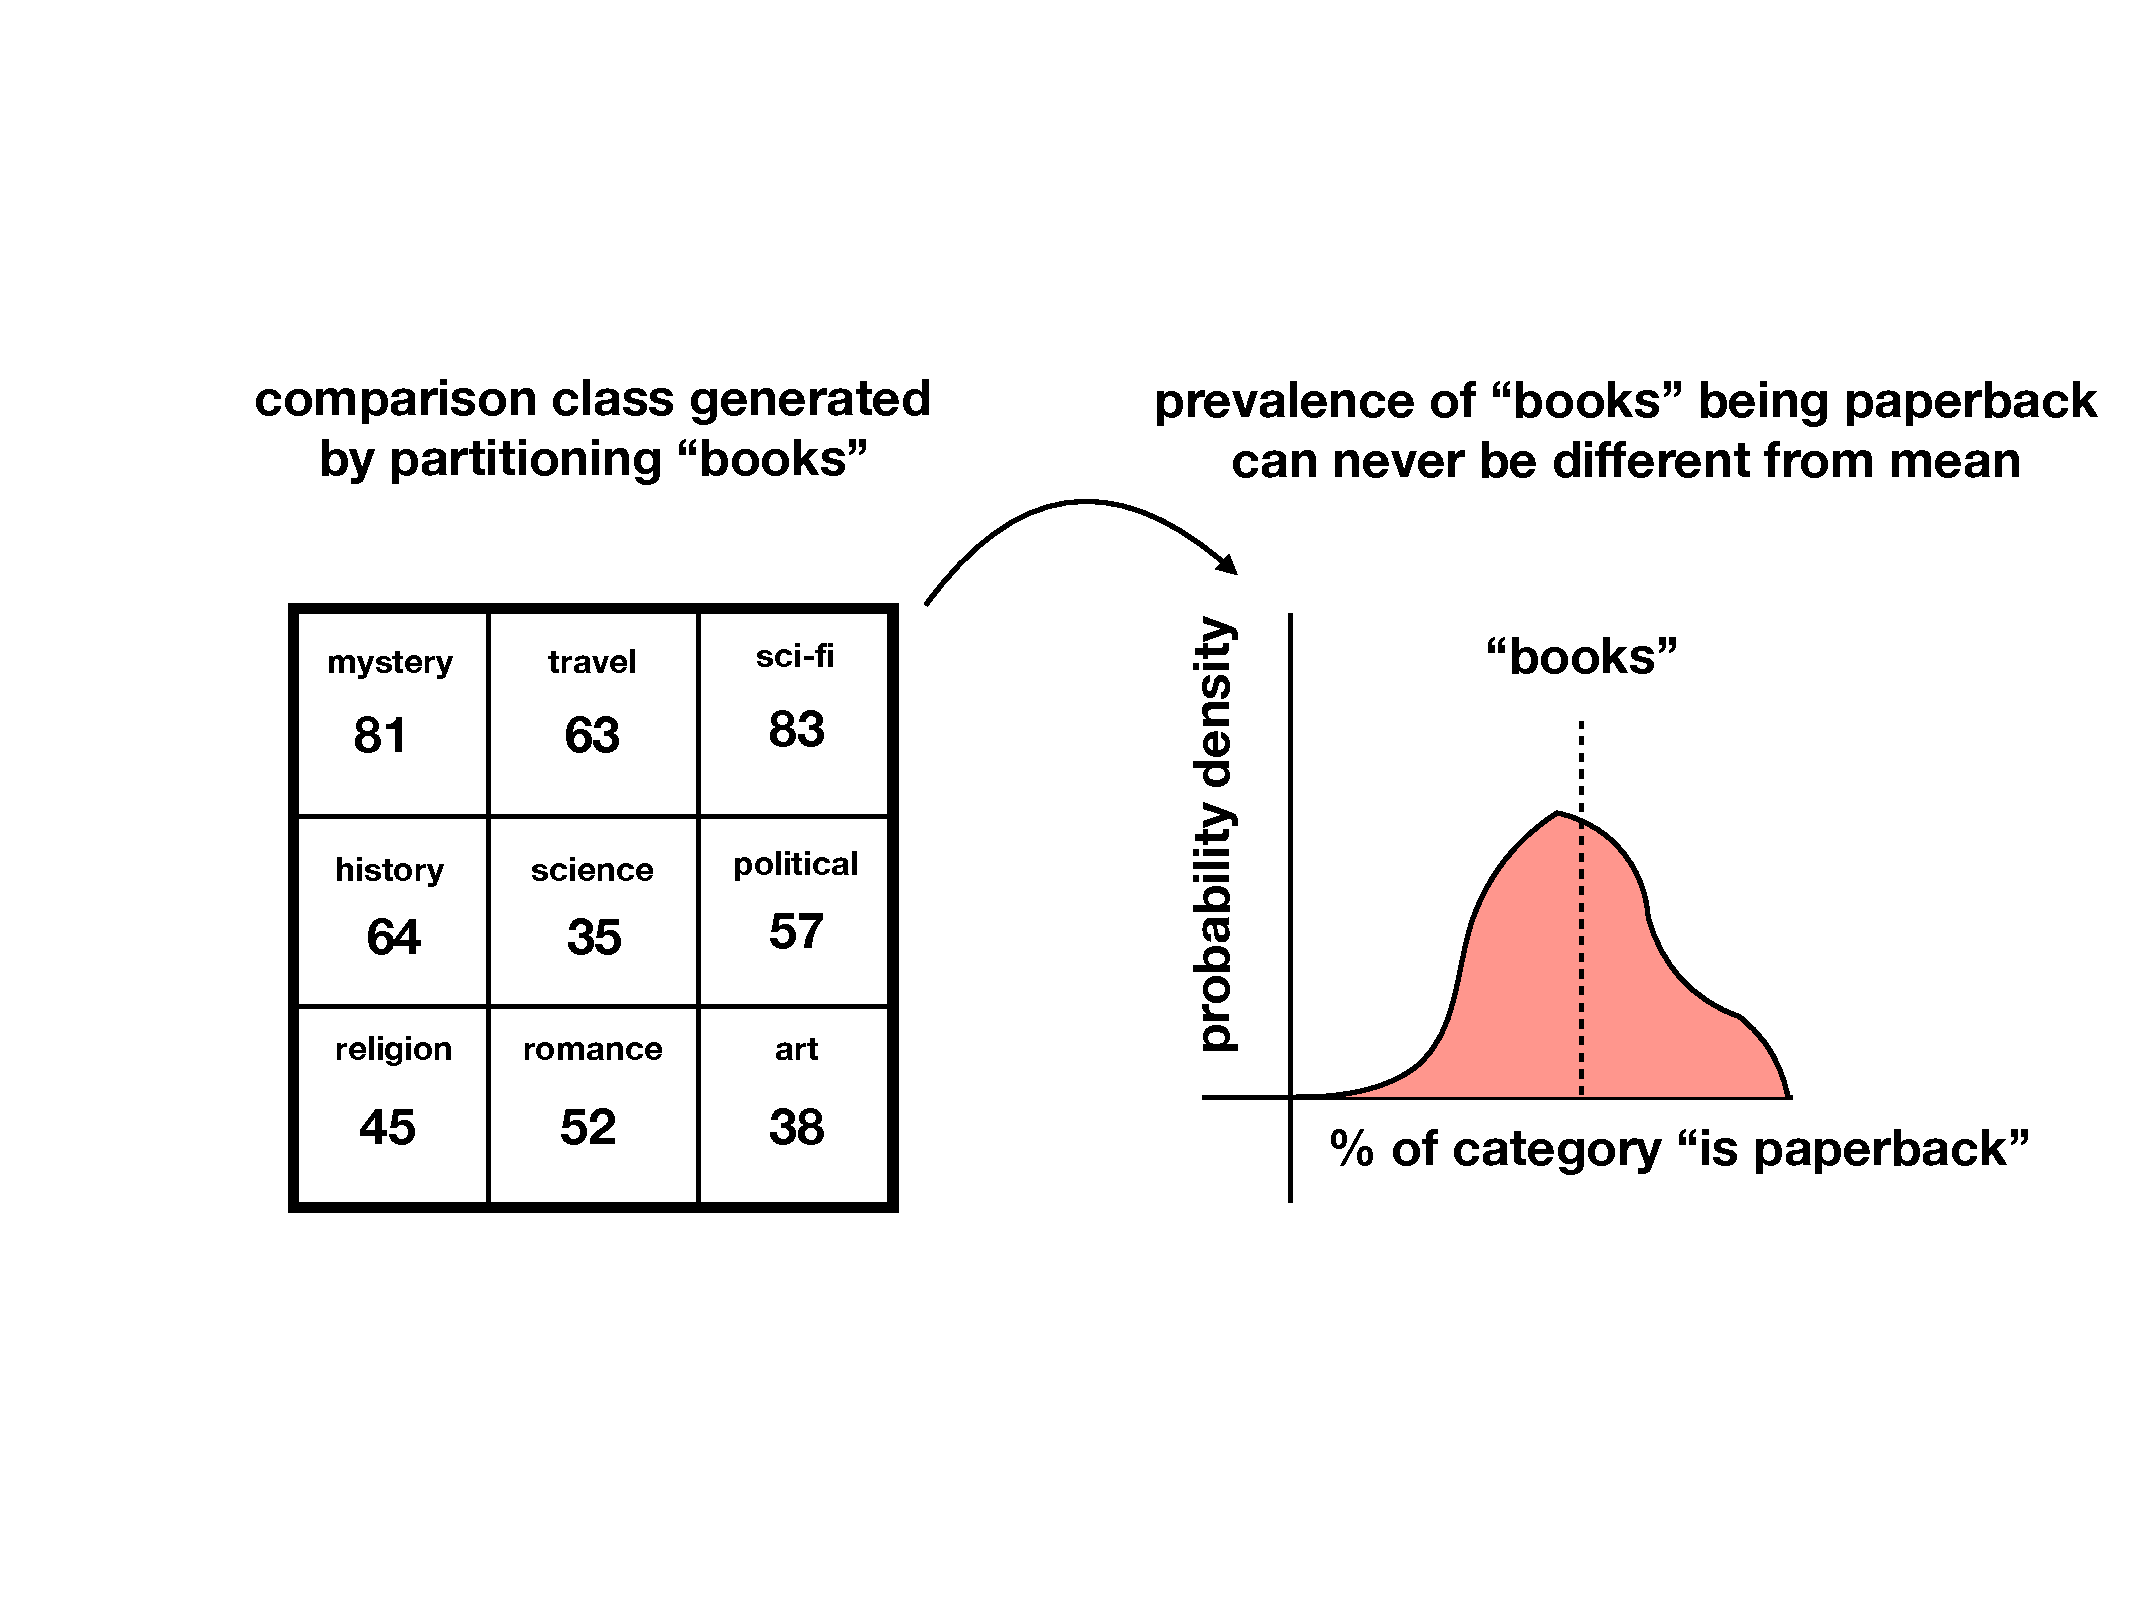
\includegraphics{figs/books-paperbacks.pdf}
\caption{\label{fig:booksArePaperbacks}Sketch of an argument for why
\enquote{Books are paperbacks} sounds odd. The feature \enquote{is
paperback} can only be predicated (in the sense of Keil (1979)) of
individual books, which are organized into collections (here, by genre).
The prevalence prior is constructed by aggregating these collections of
books. Then the prevalence of \enquote{is paperbook} for the category of
\enquote{books} can never be higher than the mean of the prior
distribution. The endorsement model would give this sentence a rating of
0.5, corresponding to neither true nor false.}
\end{figure}

Imagine there is a job in the local beaurocrat's office to handle the
mail from Antarctica and this job is assigned to Mary; to date, however,
there has never been any mail from Antarctica (Cohen, 1999). That is,
the statement \enquote{Mary has handled mail from Antarctica} is false.
Sentence (2) is still thought to be true despite zero actual instances
of the event. We think (2) is a boundary case of generalizations
expressing predictive probabilities, which we elucidated in Expt. 2c. In
in that study, we experimentally dissociated predictive probability from
past frequency, and saw that only a model that took into account
predictive probability could explain participants' endorsements of
generalizations. We expect the same to be true here, elucidated by the
intuition that: were there to be any mail coming from Antarctica, Mary
would handle it. Past frequency or actual prevalence in the world often
tracks predictive probabilities, but language users' internal models of
how the world works can lead them in certain situations to expect
something different in the future.

Our focus on predictive probability makes even new prediction about some
classic puzzles. Sentence (3) is the conceptual opposite of sentence
(2). Imagine that currently every Supreme Court Justice has a social
security number which is an \emph{even number}. Sentence (3) is still
considered false, every though the property holds in 100\% of the
category (Cohen, 1999). We predict this phenomenon is the result of
abstract, intuitive theories guiding us to reject observed frequencies
in forming our subjective probabilities. That is, because observers
strongly believe selection for the Supreme Court is not influenced by
one's social security number, speakers would assign a roughly 50\%
subjective probability that the \emph{next} justice would have an even
social security number. Then, given that the all professions would have
roughly the same probability of having employees with even social
security numbers, Sentence (3) is again similar to \enquote{Birds are
female}. However, were we to learn much more surprising
information---for instance, if every Supreme Court Justice in U.S.
history had a social security number which was a \emph{prime
number}---the shear suspiciousness could compel an observer to revise
their theory of the domain (appealing perhaps to a conspiracy), update
their subjective probability of future instances, and then accept the
generic. That is, we predict there are situations where statements like
(3) could be considered felicitious generalizations.

Understanding how a semantic representation \emph{composes} is another
critical test for a theory of generalizations in language. Nickel (2008)
suggests Sentence (4) is semantically equivalent to: \enquote{Elephants
live in Africa and elephants live in Asia}. Stastistical account of
generalizations have trouble with this kind of conjunction: It cannot be
the case that \emph{most} (more than half) elephants live in Africa and
\emph{most} (more than half) elephants live in Asia, unless we are to
posit \emph{international elephants} (i.e., individual elephants who
live part-time in Africa and part-time in Asia), which we would rather
not have to posit. However, this is the only interpretation if the
generalization is given a fixed, majority based quantificational account
(e.g., if the generic means \emph{most}). Our theory does not provide a
fixed semantics for the generalizations, but an uncertain one, which can
be updated as more information comes in. In fact, with a strong
constraint against the existence of \emph{international elephants} but
with any further semantic assumptions, our model infers that some
elephants live in Africa and other lives in Asia.\footnote{An
  implementation of this example can be found:
  \url{http://forestdb.org/models/generics-conjunction.html}.}
Importantly, the model believes that most lives in Africa, when it only
hears that \enquote{Elephants live in Africa}, and only later revises
it's beliefs to a weaker \enquote{some}-like interpretation after
hearing they live in Asia as well. Our model flexibly accomodates new
evidence that might otherwise contradict previous utterances because it
maintains uncertainty about the precise interpretation of single
utterances.

Finally, sometimes a property is widespread relative to other kinds or
groups, and it might be so systemic that we would believe it to be the
case in the future, but speakers still might find it avertise to
actually endorse the generalization. Such is the situation with Sentence
(5) (Haslanger, 2011). Due of a variety of socio-cultural reasons,
Haslanger (2011) argues that women tend to be submissive (more so than
men, and many other social categories), yet still cautions against
asserting (5). In our \textbf{Model Simulations} section, we showed that
the genearlization often implies the property is widespread, even with
relatively uninformed prior beliefs about the property. If the generic
conveys the property is in fact more widespread than the speaker herself
might believe, this can lead to a distortion of the truth..\footnote{Note
  that this can straight-forwardly capture the central phenomena of
  Cimpian et al. (2010).} The current formulation of the model is
relatively ambivalent about the deviations of the listener's beliefs
from the speaker's belief (i.e., the speaker doesn't mind that the
prevalence that she believes to be true will be exaggerated in the mind
of the listener). However, if states of the world (or, listener's
beliefs about states of the world) correspond to different subjective
values, speakers who take into the account the subjective utilities of
the listener may produce language that deviates from what a pure
informational transmission speaker might say. This kind of extension to
rational models of communication has already been used to account for a
variety of phenomena in \emph{polite language} use (Yoon, Tessler,
Goodman, \& Frank, 2016, 2017). We propose adopting such a value-based
utility structure for states of the world for language about social
categories: If the speaker found states of the world where the
probability of the feature is high (e.g., a world where many women were
submissive) as undesirable, then a speaker who considered both the
informational content of the utterance and the utility in the states of
the world implied by that utterance would too find it reprehensible to
make such a generalization. We find this possibilitity intruiging and
leave it for future work.

In sum, we've tried to argue that our information-theoretic
communicative model couched in general cognitive framework can be used
to explain a number of interesting and heretofore puzzling phenomena in
genericity as well as make novel predictions about a wider range of
language. The precise implementation of these hypotheses we leave for
future work.

\subsection{Relationship to other
theories}\label{relationship-to-other-theories}

To our knowledge, the present papaer presents the first formal theory of
genericity in language that makes accurate and precise quantitative
predictions about human behavioral data. A number of other theories of
genericity have been proposed in the linguistics and psychological
literatures. We now turn to situating our account with respect to these
previous theories. Semantic theories fall into one of two broad camps:
Those that appeal to the statistics of the world (e.g., how many Ks have
F) and those that appeal to structured, conceptual representations
(e.g., \emph{there is something about being K which causes it to F}).
Statistical and conceptual theories express the major contrasting views
of the truth conditions of generic statements (Carlson, 1995).\footnote{We
  use the terms statistical and conceptual to refer to what Carlson
  (1995) referred to as \enquote{inductive} and \enquote{rules and
  regulations} views, respectively.}

\subsubsection{Statistical accounts}\label{statistical-accounts}

\paragraph{Relative and absolute
generics}\label{relative-and-absolute-generics}

Our underspecified threshold model has clear antecedents in other
statistical accounts, most notably Cohen (1999) 's theory of generics as
a frequency adverb (e.g., \enquote{generally}). For Cohen, the statement
\enquote{Birds lay eggs} means \enquote{Generally, birds lay eggs}, and
then he takes up the task of explaining what \enquote{generally} means.
He partitions generics into two types: \emph{absolute} and
\emph{relative} generics. \emph{Absolute generics} use a fixed, 50\%
threshold on prevalence: \(P(F\mid K)>0.5\). Roughly speaking,
\enquote{Dogs have four legs} is true because a given dog is more likely
than not to have four legs. \emph{Relative generics} depend upon an
alternative set of kinds (his notation: \(Alt(K)\)), analogous to our
comparison class. \enquote{Mosquitos carry malaria} is a relative
generic: it is true because an arbitrary mosquito is more likely than an
arbitrary member of an alternative kind to have the feature.

Our uncertain-threshold model deviates from Cohen's account in two
primary ways. First, though his theory is framed in terms of
probabilities, it still utilities a fixed threshold semantics and thus
is only able to make predictions about what is \enquote{true} and what
is \enquote{false}. In our theory, there is uncertainty about the core
semantic meaning, and this uncertainty (though reduced in context)
drives the model to make graded predictions about endorsement. Second,
Cohen draws an \emph{a priori} distinction between \emph{Absolute} and
\emph{Relative} generics, and provides different mechanisms for each
each. We used examples of both in our stimuli (Expt. 1) and found that
our single model handles both without any addition assumptions, casting
doubt on the \emph{a priori} distinction between \enquote{absolute} and
\enquote{relative.}\footnote{For a related theory that aims to do away
  with the distinction between \enquote{absolute} and \enquote{relative}
  adjectives, see Lassiter and Goodman (2015).}

We note additional machinery that Cohen's theory relies upon (and that
is not currently required in our account) to explain the
context-sensitivity of generics: contextually restricting the entities
that go into the computation of prevalence (i.e., which robins do we
look at to compute the probability of \emph{laying eggs} among
\emph{robins}?). His theory posits that prevalence is calculuated by
only considering entities that \emph{could have some feature} in a
contextually-specified alternative set of features (so called
\(Alt(F)\)). For example, the property \enquote{lays eggs} induces a set
of alternatives that are associated with mechanisms of reproduction
(e.g., \enquote{gives birth to live young}, \enquote{undergoes mitosis},
\ldots{}). Therefore, \enquote{Robins lay eggs} is evaluated as an
\emph{absolute generic} because only individuals that are female members
of kinds are under consideration, because only the female members can
plausibly satisfy one of the other aternatives having to do with
reproduction (i.e., the alternative features in \(Alt(F)\)). The
inferential machinery behind Cohen's domain restriction (i.e., what
comrpises \(Alt(F)\)?) relies upon conceptual information, but the
details remain obscure (Carlson, 1995).\footnote{However, see Cohen
  (2004) for a discussion of how his semantic constraints relate to
  different kinds of generics and different kinds of conceptual
  representational frameworks found in cognitive science.} However, we
note that this mechanism may be implicit in our own theory: the prior
distribution over the prevalence of \emph{lays eggs} presumably includes
aspects of people's theories about reproduction (i.e., that only females
lay eggs). Thus, there may exist a refactorization of the uncertain
threshold model to a fixed threshold where the listener has uncertainty
about the relevant domain restriction.

\paragraph{\texorpdfstring{\enquote{Normal}
accounts}{Normal accounts}}\label{normal-accounts}

The primary alternative view under the statistical banner draws on the
intuition that generics express something normative in the world (Asher
\& Morreau, 1995; Nickel, 2008; F. J. Pelletier \& Asher, 1997). For
example, \enquote{Dogs have four legs} is a good generalization even
though, regrettably, not all dogs have four legs. However, were the
world to function \emph{normally} (e.g., dogs would not be involved in
freak-tractor accidents or be born with strange genetic mutations), then
\emph{all} dogs would have four legs. The idea that our beliefs about
what is normal in the world influences our judgments about
generalizations has intuitive appeal for rejecting accidentally true
generalizations (e.g., \enquote{Supreme Court justices have even social
security numbers}; described above) and stereotyped language (e.g.,
\enquote{Boys are good at math}). Our theory does not directly formalize
\enquote{what is normal}, though we argue that a speaker's beliefs about
what is \emph{probable} (which may relate to what is \emph{normal}; see
Icard, Kominsky, \& Knobe, 2017) plays a role in endorsing and
interpreting generalizations. We showed in Expt. 2c that a speaker's
beliefs about what is likely to be the case in the near future matters
above and beyond what is currently true in the world for endorsing
generalizations. Our notion of prevalence is as a predictive
probability, which incorporates background knowledge in order to make
predictions about the future.

\paragraph{Underquantification}\label{underquantification}

A proposal similar to our account concerning underspecification of
generics has been made in the computational linguistics literature
(so-called \emph{underquantification}; Herbelot \& Copestake, 2011). In
their model, generics express an explicit quantified relation,
specifically either \enquote{Some}, \enquote{Most}, or \enquote{All}.
The task of the computational linguist, then, is to construct a set of
features that accurately predicts (relative to human judgments) the
quantified relationship expressed by the generic (Cimpian et al., 2010;
analagous to a quantifier version of the \emph{implied prevalence} task
used in Gelman \& Raman, 2003). Our semantic theory can be seen as a
generalization of the \emph{underquantification} to a continuous
interval of possible meanings. This distinction is relevant for the
acquisition of the language of generalizations; we do not think that
quantified relations (e.g., \enquote{Some}, \enquote{All}) are in any
way primary or special. Additionally, by using a vague, underspecified
threshold, our formulation naturally extends to other scales and other
kinds of generalizations (e.g., habitual language), where quantified
relations like \enquote{Most} or \enquote{All} are not directly
applicable.

\paragraph{Generic as indexical}\label{generic-as-indexical}

Sterken (2015) has recently proposed an intruiging account of the
context-sensitive of generic language by treating generics as a kind of
\emph{indexical} (e.g., \enquote{this} or \enquote{I}). The variability
of endorsements is then attributed to mechanisms of domain restriction
(described above with Cohen (1999)) and context-sensitive
\enquote{quantificational force}. Our uncertain-threshold semantics may
be a precise formalization of Sterken (2015)'s \enquote{quantificational
force} (and a generalization of \emph{underquantification}, see above),
and we have argued above that domain restriction is not a necessary
mechanisms for the cases considered in this paper. We leave for future
work exploring how the context-sensitivity of an indexical may differ
from the kind of context-sensitivity in our model.

\subsubsection{Conceptual accounts}\label{conceptual-accounts}

Conceptual accounts of generics emphasize the structure of generic
knowledge (Prasada, 2000), and view generic utterances as the way of
expressing special mental relationships between kinds and properties
(Leslie, 2008; Prasada et al., 2012). These accounts start with the
perspective that generics express rich, conceptual relationships between
kinds and properties. That is, \enquote{Bishops move diagonally} not
because of a statistical relationship, but rather, because those are the
rules of the game; if you start moving the bishop other ways besides
diagonally, you cease to be playing chess. If a lion lacked the capacity
to roar, we might consider a less good example of being a lion because
\enquote{lions roar}.

The most influential conceptual account of generics is from Leslie
(2007). For Leslie, generics are tied to the cognitive system's
\enquote{default mode of generalization}, which infants seem ready to
make use of by drawing strong generalizations from small amounts of data
(e.g., Baldwin, Markman, \& Melartin, 1993). Leslie's \enquote{default
mode} comes equipped with the ability to single-out
\emph{striking properties} (e.g., properties which are dangerous or
appalling) as particularly useful aspects of the world to know about.
Hence, \enquote{Mosquitos carry malaria} is true because malaria can
kill you and is useful to know about.

This accounts predicts that generics that convey striking properties
should be endorsed even when they are relatively rare in the category
(i.e., low referent-prevalence; e.g., \enquote{Sharks attack swimmers}).
Indeed, naturalistic examples (e.g., \enquote{Sharks attack swimmers})
and artificial examples (e.g., \enquote{Lorches have purple feathers})
supplemented with striking information (e.g.,\enquote{These feathers are
as sharp as needles and can easily get lodged in you, causing massive
bleeding}) are endorsed when the prevalence is quite low (e.g., 30\% of
lorches have purple feathers; Cimpian et al. (2010); see Expt. 1 for
naturalistic cases). In pilot work, using a paradigm similar to the
prior manipulation paradigm employed in the causal language experiments
(Expt. 3a), we have observed that the prior distribution over the
prevalence \(P(h)\) change when supplied information about the
dangerousness of the feature. That is, our pilot work suggests that
experiments that experimentally induce beliefs about the dangerousness
of a feature also manipulate the prevalence priors. Thus, our model
would also predict these effects, but by way of the prevalence priors
rather than some direct connection between generics and striking
features.

Of course, not all generics convey striking or appalling information
(e.g., \enquote{Birds lay eggs}). Leslie's default mode, thus, also
distinguishes \emph{negative counter-instances} of a property (e.g., a
bird that doesn't lay eggs, such as a male bird) from \emph{positive
counter-instances} (e.g., a hypothetical bird that bears live young) The
conceptual account argues that generics are much less reasonable when
\emph{positive} counter-instances exist. For example, \enquote{Birds are
female} seems weird because \emph{being male} is a \emph{positive}
counter-instance of \emph{being female}, but since there are no birds
that bear live young (i.e., no \emph{positive counter-instances}),
\enquote{Birds lay eggs} is fine. In the current version of our theory,
both kinds of counter-instances influence the referent-category
feature-probabilities, though only positive counter-instances could
impact the statistical details of the comparison class (in particular,
when constructed with respect to the feature; see discussion about the
Comparison Class). Thus, the notion of \emph{positive} and
\emph{negative} counter-instances may result from a particular way of
looking at the constructs posited in our model, namely prevalences
within- and across- categories or features.

Finally, generics are not limited to conveying rich, conceptual
information; they are also used to describe facts of the world.
\enquote{Ravens are bigger than toasters} is a true statement, but not
because of a rich relationship between ravens and toasters.
\enquote{Barns are red} because most barns are red. If farmers around
the world decided to paint their barns green, the things they would be
painting would still be barns; in that world, we might say
\enquote{Barns are green}. Thus, conceptual accounts must be
supplemented with the proviso that in ceratin situations, the statistics
of the world are relevant.

Our view is that subjective probabilities can be formed either from
worldly observations or because of the structure of people's mental
representations. In the last fifteen years, there has been tremendous
progress in formalizing Rich, structural mental representations can be
formalized in probabilistic models, which can be used to derive
quantitative predictions about inferences derived from that knowledge
(Tenenbaum, Kemp, Griffiths, \& Goodman, 2011). For example, Kemp and
Tenenbaum (2008) introduced a model for learning different kinds of
structural relationships between objects and properties (e.g.,
taxonomies, social cliques, dominance relations). Goodman et al. (2015)
argue that concepts and intuitive theories can be constructed from
elementary random primitives using insights from \emph{probabilistic
programmming}.

In this paper, we take a minimalist approach to modeling conceptual
structure, incorporating only what is necessary into the interpreter's
background knowledge, the prior on prevalence \(P(h)\). In our Bayesian
data analysis of background knowledge, we use a mixture model that
reflects basic knowledge about kinds and properties (e.g., that most
kinds don't have most properites).\\
It's plausible that more richly structured knowledge of the kind
described by Prasada et al. (2013) and Leslie (2007) can be
incorporating into the general probabilsitic framework that we use here.

The key point of divergence then between the conceptual accounts and our
view concerns the core, semantic meaning of a generic statement.
Conceptual accounts try to identify the core meaning of a generalization
directly with aspects of conceptual structure. For us, the semantics
concerns a probability, which is the byproduct of a conceptual
structure, but it is not the conceptual structure itself. We believe
this provides a more unifying view of generics, giving a single metric
as the basic currency of generic meaning: probability.

\section{Conclusion}\label{conclusion}

It might seem paradoxical that a part of language that is so common in
communication and central to learning should be vague. Shouldn't
speakers and teachers want to express their ideas as crisply as
possible? To the contrary, underspecification can be efficient, given
that context can be used to resolve uncertainty in meaning (Piantadosi,
Tily, \& Gibson, 2012). In our work, context takes the form of shared
beliefs about the property in question. By leveraging this common
ground, genericity provide a powerful way to communicate and learn
generalizations, which would otherwise be difficult or costly
information to learn through direct experience.

The dark side of this flexibility is the potential for miscommunication
or deceit: A speaker might assert a generalization that she herself
would not accept, conveying a too-strong generalization to a naive
listener. Our model predicts this potential particularly for properties
which, when present, are widespread in a category; biological properties
are believed to have this distribution, but many properties of social
categories may as well (Cimpian \& Markman, 2011; Cimpian, Mu, \&
Erickson, 2012; Rhodes et al., 2012). Disagreements are also predicted
when interlocutors fail to share background assumptions, which could be
differences in the prior distributions on prevalence or the comparison
class. Core aspects of political disagreement then (e.g., as to whether
\enquote{Humans cause global warming}) could be derived from differences
in the estimated causal responsibility of the category in question
(e.g., what impacts humans are having), of \emph{other forces} (e.g.,
plate tectonics), as well as the comparison class of other forces (e.g.,
what are the alternative causes?). This is a promising area for future
research.

Categories are inherently unobservable. You cannot see the category
\textsc{dog}, only some number of instances of it. Yet we easily talk
about these abstractions, conveying hard-won generalizations to each
other and down through generations. The theory presented here provides
the first computational perspective on how we communicate
generalizations and how beliefs play a central role in the meaning of
words.

\newpage

\section{References}\label{references}

\hypertarget{refs}{}
\hypertarget{ref-Asher1995}{}
Asher, N., \& Morreau, M. (1995). What some generic sentences mean.
\emph{The Generic Book}, 300--338.

\hypertarget{ref-Baldwin1993}{}
Baldwin, D. A., Markman, E. M., \& Melartin, R. L. (1993). Infants '
Ability to Draw Inferences about Nonobvious Object Properties: Evidence
from Exploratory Play. \emph{Child Development}, \emph{64}(3), 711--728.

\hypertarget{ref-Bale2011}{}
Bale, A. C. (2011). Scales and comparison classes. \emph{Natural
Language Semantics}, \emph{19}, 169--190.

\hypertarget{ref-Behrens2005}{}
Behrens, L. (2005). Genericity from a cross-linguistic perspective.
\emph{Linguistics}, \emph{43}(2), 275--344.

\hypertarget{ref-Bergen2016}{}
Bergen, L., Levy, R., \& Goodman, N. D. (To appear). Pragmatic reasoning
through semantic inference. \emph{Semantics and Pragmatics}.

\hypertarget{ref-Brandone2014}{}
Brandone, A. C., Gelman, S. A., \& Hedglen, J. (2014). Children's
Developing Intuitions About the Truth Conditions and Implications of
Novel Generics Versus Quantified Statements. \emph{Cognitive Science},
1--28.

\hypertarget{ref-Carlson1977}{}
Carlson, G. N. (1977). \emph{Reference to kinds in english}
(PhD thesis). University of Massachusetts, Amherst.

\hypertarget{ref-Carlson1995essay}{}
Carlson, G. N. (1995). Truth conditions of generic sentences: Two
contrasting views. In G. N. Carlson \& F. J. Pelletier (Eds.), \emph{The
generic book} (pp. 224--38). Chicago: University of Chicago Press.

\hypertarget{ref-Carlson1995}{}
Carlson, G. N., \& Pelletier, F. J. (1995). \emph{The generic book.}
Chicago, IL: Chicago University Press.

\hypertarget{ref-Cheng1997}{}
Cheng, P. W. (1997). From Covariation to Causation: A Causal Power
Theory. \emph{Psychological Review}, \emph{104}(2), 367--405. Retrieved
from \url{http://psycnet.apa.org/fulltext/1997-03612-007.pdf}

\hypertarget{ref-Cheng1992}{}
Cheng, P. W., \& Npvick, L. R. (1992). Covariation in Natural Causal
Induction. \emph{Psychological Review}, \emph{99}(2), 365--382.
Retrieved from \url{http://psycnet.apa.org/fulltext/1992-26096-001.pdf}

\hypertarget{ref-Cimpian2008}{}
Cimpian, A., \& Markman, E. M. (2008). Preschool children's use of cues
to generic meaning. \emph{Cognition}, \emph{107}, 19--53.
doi:\href{https://doi.org/10.1016/j.cognition.2007.07.008}{10.1016/j.cognition.2007.07.008}

\hypertarget{ref-Cimpian2011a}{}
Cimpian, A., \& Markman, E. M. (2011). The Generic/Nongeneric
Distinction Influences How Children Interpret New Information About
Social Others. \emph{Child Development}, \emph{82}(2), 471--492.
doi:\href{https://doi.org/10.1111/j.1467-8624.2010.01525.x}{10.1111/j.1467-8624.2010.01525.x}

\hypertarget{ref-Cimpian2007}{}
Cimpian, A., Arce, H.-M. C., Dweck, C. S., \& Markman, E. M. (2007).
Subtle Linguistic Cues Affect Children's Motivation. \emph{Psychological
Science}, \emph{18}(4), 314--316.

\hypertarget{ref-Cimpian2010}{}
Cimpian, A., Brandone, A. C., \& Gelman, S. A. (2010). Generic
statements require little evidence for acceptance but have powerful
implications. \emph{Cognitive Science}, \emph{34}(8), 1452--1482.

\hypertarget{ref-Cimpian2012b}{}
Cimpian, A., Mu, Y., \& Erickson, L. C. (2012). Who Is Good at This
Game? Linking an Activity to a Social Category Undermines Children's
Achievement. \emph{Psychological Science}, \emph{23}(5), 533--541.
doi:\href{https://doi.org/10.1177/0956797611429803}{10.1177/0956797611429803}

\hypertarget{ref-Cohen1999}{}
Cohen, A. (1999). Generics, Frequency Adverbs, and Probability.
\emph{Linguistics and Philosophy}, \emph{22}.

\hypertarget{ref-Cohen2004}{}
Cohen, A. (2004). Generics and Mental Representations. \emph{Linguistics
and Philosophy}, \emph{27}(5), 529--556.
doi:\href{https://doi.org/10.1023/B:LING.0000033851.25870.3e}{10.1023/B:LING.0000033851.25870.3e}

\hypertarget{ref-Cree2006}{}
Cree, G. S., McNorgan, C., \& McRae, K. (2006). Distinctive features
hold a privileged status in the computation of word meaning:
Implications for theories of semantic memory. \emph{Journal of
Experimental Psychology. Learning, Memory, and Cognition}, \emph{32}(4),
643--658.
doi:\href{https://doi.org/10.1037/0278-7393.32.4.643}{10.1037/0278-7393.32.4.643}

\hypertarget{ref-Degen2014}{}
Degen, J., \& Goodman, N. D. (2014). Lost your marbles? The puzzle of
dependent measures in experimental pragmatics. In \emph{Proceedings of
the thirty-sixth annual conference of the Cognitive Science Society}.

\hypertarget{ref-Dewar2010}{}
Dewar, K. M., \& Xu, F. (2010). Induction, overhypothesis, and the
origin of abstract knowledge: Evidence from 9-month-old infants.
\emph{Psychological Science}, \emph{21}, 1871--1877.
doi:\href{https://doi.org/10.1177/0956797610388810}{10.1177/0956797610388810}

\hypertarget{ref-Frank2012}{}
Frank, M. C., \& Goodman, N. D. (2012). Predicting pragmatic reasoning
in language games. \emph{Science}, \emph{336}(6084).

\hypertarget{ref-Franke2014cogsci}{}
Franke, M. (2014). Typical use of quantifiers: A probabilistic speaker
model. In \emph{Proceedings of the 36th annual meeting of the cogntiive
science society} (pp. 1--6). Retrieved from
\href{http://staff.science.uva.nl/\%7B~\%7Dmfranke/Papers/Franke\%7B/_\%7D2014\%7B/_\%7DTypical\%20use\%20of\%20quantifiers\%20A\%20probabilistic\%20speaker\%20model.pdf}{http://staff.science.uva.nl/\{\textasciitilde{}\}mfranke/Papers/Franke\{\textbackslash{}\_\}2014\{\textbackslash{}\_\}Typical use of quantifiers A probabilistic speaker model.pdf}

\hypertarget{ref-Gelman2003}{}
Gelman, S. A. (2003). \emph{Essential child: Origins of
essentialntialism in everyday thought.} Oxford University Press.

\hypertarget{ref-Gelman2004}{}
Gelman, S. A. (2004). Learning words for kinds: Generic noun phrases in
acquisition. In \emph{Weaving a lexicon} (pp. 445--484). MIT Press.

\hypertarget{ref-Gelman1999}{}
Gelman, S. A., \& Heyman, G. D. (1999). Carrot-Eaters and
Creature-Believers: The Effects of Lexicalization on Children's
Inferences About Social Categories. \emph{Psychological Science},
\emph{10}(6), 489--493.
doi:\href{https://doi.org/10.1111/1467-9280.00194}{10.1111/1467-9280.00194}

\hypertarget{ref-Gelman2003b}{}
Gelman, S. A., \& Raman, L. (2003). Preschool children use linguistic
form class and pragmatic cues to interpret generics. \emph{Child
Development}, \emph{74}(1), 308--325.

\hypertarget{ref-Gelman1998}{}
Gelman, S. A., Coley, J. D., Rosengren, K. S., Hartman, E., \& Pappas,
A. (1998). Beyond labeling: the role of maternal input in the
acquisition of richly structured categories. \emph{Monographs of the
Society for Research in Child Development}, \emph{63}(1), I--V,
1--148;discussion 149--157.

\hypertarget{ref-Gelman2008}{}
Gelman, S. A., Goetz, P. J., Sarnecka, B. W., \& Flukes, J. (2008).
Generic Language in Parent-Child Conversations. \emph{Language Learning
and Development}, \emph{4}(1), 1--31.
doi:\href{https://doi.org/10.1080/15475440701542625.Generic}{10.1080/15475440701542625.Generic}

\hypertarget{ref-Gelman2015}{}
Gelman, S. A., Leslie, S.-J., Was, A. M., \& Koch, C. M. (2015).
Children's interpretations of general quantifiers, specific quantifiers
and generics. \emph{Language, Cognition and Neuroscience}, \emph{30}(4),
448--461.
doi:\href{https://doi.org/10.1080/23273798.2014.931591}{10.1080/23273798.2014.931591}

\hypertarget{ref-GelmanEtAl2004}{}
Gelman, S. A., Taylor, M. G., Nguyen, S. P., Leaper, C., \& Bigler, R.
S. (2004). Mother-child conversations about gender: Understanding the
acquisition of essentialist beliefs. \emph{Monographs of the Society for
Research in Child Development}, \emph{69}(1), vii, 116--127.
doi:\href{https://doi.org/10.1111/j.1540-5834.2004.06901001.x}{10.1111/j.1540-5834.2004.06901001.x}

\hypertarget{ref-Gerstenberg2015how}{}
Gerstenberg, T., Goodman, N. D., Lagnado, D. A., \& Tenenbaum, J. B.
(2015). How, whether, why: Causal judgments as counterfactual contrasts.
In D. C. Noelle, R. Dale, A. S. Warlaumont, J. Yoshimi, J. Matlock T.,
C. D., \& P. P. Maglio (Eds.), \emph{Proceedings of the 37th Annual
Conference of the Cognitive Science Society} (pp. 782--787). Austin, TX:
Cognitive Science Society.

\hypertarget{ref-Goodman2016}{}
Goodman, N. D., \& Frank, M. C. (2016). Pragmatic language
interpretation as probabilistic inference. \emph{Trends in Cognitive
Sciences}.

\hypertarget{ref-dippl}{}
Goodman, N. D., \& Stuhlmüller, A. (2014). The Design and Implementation
of Probabilistic Programming Languages. \url{http://dippl.org}.

\hypertarget{ref-Goodmanconcepts}{}
Goodman, N. D., Tenenbaum, J. B., \& Gerstenberg, T. (2015). Concepts in
a probabilistic language of thought. In \emph{The conceptual mind: New
directions in the study of concepts}. MIT Press.

\hypertarget{ref-Gopnik2003theory}{}
Gopnik, A. (2003). The theory theory as an alternative to the innateness
hypothesis. \emph{Chomsky and His Critics}, 238--254.

\hypertarget{ref-Griffiths2005}{}
Griffiths, T. L., \& Tenenbaum, J. B. (2005). Structure and strength in
causal induction. \emph{Cognitive Psychology}, \emph{51}(4), 334--84.
doi:\href{https://doi.org/10.1016/j.cogpsych.2005.05.004}{10.1016/j.cogpsych.2005.05.004}

\hypertarget{ref-Griffiths2009}{}
Griffiths, T. L., \& Tenenbaum, J. B. (2009). Theory-Based Causal
Induction. \emph{Psychological Review}, \emph{116}(4), 661--716.
doi:\href{https://doi.org/10.1037/a0017201}{10.1037/a0017201}

\hypertarget{ref-Gweon2010}{}
Gweon, H., Tenenbaum, J. B., \& Schulz, L. E. (2010). Infants consider
both the sample and the sampling process in inductive generalization.
\emph{Proceedings of the National Academy of Sciences of the United
States of America}, \emph{107}(20), 9066--71.
doi:\href{https://doi.org/10.1073/pnas.1003095107}{10.1073/pnas.1003095107}

\hypertarget{ref-Haslanger2011}{}
Haslanger, S. (2011). Ideology, generics, and common ground. In
\emph{Feminist metaphysics} (pp. 179--207). Springer.

\hypertarget{ref-Henrich2015}{}
Henrich, J. (2015). \emph{The secret of our success: how culture is
driving human evolution, domesticating our species, and making us
smarter}. Princeton University Press.

\hypertarget{ref-Herbelot2011}{}
Herbelot, A., \& Copestake, A. (2011). Formalising and specifying
underquantification Quantification resolution. In \emph{IWCS} (pp.
165--174).

\hypertarget{ref-HumeTHN}{}
Hume, D. (1888). (L. A. Selby Bigge, Ed.). Oxford, Clarendon Press.

\hypertarget{ref-Icard2017}{}
Icard, T. F., Kominsky, J. F., \& Knobe, J. (2017). Normality and actual
causal strength. \emph{Cognition}, \emph{161}, 80--93.
doi:\href{https://doi.org/10.1016/j.cognition.2017.01.010}{10.1016/j.cognition.2017.01.010}

\hypertarget{ref-Keil1979}{}
Keil, F. C. (1979). \emph{Semantic and conceptual development.} Harvard
University Press.

\hypertarget{ref-Keil1992}{}
Keil, F. C. (1992). \emph{Concepts, kind, and cognitive development.}
MIT Press.

\hypertarget{ref-Kemp2008}{}
Kemp, C., \& Tenenbaum, J. B. (2008). The discovery of structural form.
\emph{Proceedings of the National Academy of Sciences of the United
States of America}, \emph{105}(31), 10687--10692.
doi:\href{https://doi.org/10.1073/pnas.0802631105}{10.1073/pnas.0802631105}

\hypertarget{ref-Kennedy2007}{}
Kennedy, C. (2007). Vagueness and grammar: the semantics of relative and
absolute gradable adjectives. \emph{Linguistics and Philosophy},
\emph{30}, 1--35.
doi:\href{https://doi.org/10.1007/s10988-006-9008-0}{10.1007/s10988-006-9008-0}

\hypertarget{ref-Khemlani2012}{}
Khemlani, S., Leslie, S.-J., \& Glucksberg, S. (2012). Inferences about
members of kinds: The generics hypothesis. \emph{Language and Cognitive
Processes}, \emph{27}(6), 887--900.
doi:\href{https://doi.org/10.1080/01690965.2011.601900}{10.1080/01690965.2011.601900}

\hypertarget{ref-KrifkaGenericBookFocus}{}
Krifka, M. (1995). Focus and the interpretation of generic sentences. In
G. N. Carlson \& F. J. Pelletier (Eds.), \emph{The generic book} (pp.
238--264). Chicago: University of Chicago Press.

\hypertarget{ref-Lassiter2013}{}
Lassiter, D., \& Goodman, N. D. (2013). Context, scale structure, and
statistics in the interpretation of positive-form adjectives. In
\emph{Semantics and Linguistic Theory (SALT) 23}.

\hypertarget{ref-Lassiter2015}{}
Lassiter, D., \& Goodman, N. D. (2015). Adjectival vagueness in a
bayesian model of interpretation. \emph{Synthese}.

\hypertarget{ref-Leslie2007}{}
Leslie, S.-J. (2007). Generics and the Structure of the Mind.
\emph{Philosophical Perspectives}, \emph{21}(1), 375--403.

\hypertarget{ref-Leslie2008}{}
Leslie, S.-J. (2008). Generics: Cognition and acquisition.
\emph{Philosophical Review}, \emph{117}(1).

\hypertarget{ref-Leslie2012a}{}
Leslie, S.-J., \& Gelman, S. A. (2012). Quantified statements are
recalled as generics: Evidence from preschool children and adults.
\emph{Cognitive Psychology}, \emph{64}(3), 186--214.
doi:\href{https://doi.org/10.1016/j.cogpsych.2011.12.001}{10.1016/j.cogpsych.2011.12.001}

\hypertarget{ref-Levinson1995}{}
Levinson, S. C. (1995). Interactional biases in human thinking. In E. N.
Goody (Ed.), \emph{Social intelligence and interaction} (pp. 221--260).
Cambridge University Press.

\hypertarget{ref-McGuire1986}{}
McGuire, W. J., \& McGuire, C. V. (1986). Differences in conceptualizing
self versus conceptualizing other people as manifested in contrasting
verb types used in natural speech. \emph{Journal of Personality and
Social Psychology}, \emph{51}(6), 1135--43.
doi:\href{https://doi.org/10.1037/0022-3514.51.6.1135}{10.1037/0022-3514.51.6.1135}

\hypertarget{ref-Montague1973}{}
Montague, R. (1973). The Proper Treatment of Quantification in Ordinary
English. In \emph{Philosophy, language, and artificial intelligence}
(pp. 141-----162). Springer. Retrieved from
\url{http://semantics.uchicago.edu/kennedy/classes/s08/semantics2/montague73.pdf}

\hypertarget{ref-Nickel2008}{}
Nickel, B. (2008). Generics and the ways of normality. \emph{Linguistics
and Philosophy}, \emph{31}(6), 629--648.
doi:\href{https://doi.org/10.1007/s10988-008-9049-7}{10.1007/s10988-008-9049-7}

\hypertarget{ref-Nickel2016}{}
Nickel, B. (2016). \emph{Between logic and the world}. Oxford: Oxford
UP; Oxford UP.

\hypertarget{ref-Nisbett1983}{}
Nisbett, R. E., Krantz, D. H., Jepson, C., \& Kunda, Z. (1983). The use
of statistical heuristics in everyday inductive reasoning.
\emph{Psychological Review}, \emph{90}(4), 339--363.
doi:\href{https://doi.org/10.1037/0033-295X.90.4.339}{10.1037/0033-295X.90.4.339}

\hypertarget{ref-pearl1988probabilistic}{}
Pearl, J. (1988). Probabilistic reasoning in intelligent systems:
Networks of plausible reasoning. Morgan Kaufmann Publishers, Los Altos.

\hypertarget{ref-Pelletier1997}{}
Pelletier, F. J., \& Asher, N. (1997). Generics and defaults. handbook
of logic and language, ed. by j. van benthem and alice gb ter meulen,
1125--1177. Cambridge: The MIT Press.

\hypertarget{ref-Piantadosi2012}{}
Piantadosi, S. T., Tily, H., \& Gibson, E. (2012). The communicative
function of ambiguity in language. \emph{Cognition}, \emph{122}(3),
280--291.
doi:\href{https://doi.org/10.1016/j.cognition.2011.10.004}{10.1016/j.cognition.2011.10.004}

\hypertarget{ref-Prasada2000}{}
Prasada, S. (2000). Acquiring generic knowledge. \emph{Trends in
Cognitive Sciences}, \emph{4}(2), 66--72.
doi:\href{https://doi.org/10.1016/S1364-6613(99)01429-1}{10.1016/S1364-6613(99)01429-1}

\hypertarget{ref-Prasada2012}{}
Prasada, S., Hennefield, L., \& Otap, D. (2012). Conceptual and
Linguistic Representations of Kinds and Classes. \emph{Cognitive
Science}, \emph{36}(7), 1224--1250.
doi:\href{https://doi.org/10.1111/j.1551-6709.2012.01254.x}{10.1111/j.1551-6709.2012.01254.x}

\hypertarget{ref-Prasada2013}{}
Prasada, S., Khemlani, S., Leslie, S.-J., \& Glucksberg, S. (2013).
Conceptual distinctions amongst generics. \emph{Cognition},
\emph{126}(3), 405--22.
doi:\href{https://doi.org/10.1016/j.cognition.2012.11.010}{10.1016/j.cognition.2012.11.010}

\hypertarget{ref-Qing2014}{}
Qing, C., \& Franke, M. (2014). Gradable adjectives, vagueness, and
optimal language use: A speaker-oriented model. In \emph{Semantics and
Linguistic Theory (SALT) 24}.

\hypertarget{ref-Repacholi1997}{}
Repacholi, B. M., \& Gopnik, A. (1997). Early reasoning about desires:
evidence from 14- and 18-month-olds. \emph{Developmental Psychology},
\emph{33}(1), 12--21.
doi:\href{https://doi.org/10.1037/0012-1649.33.1.12}{10.1037/0012-1649.33.1.12}

\hypertarget{ref-Rhodes2012}{}
Rhodes, M., Leslie, S.-J., \& Tworek, C. M. (2012). Cultural
transmission of social essentialism. \emph{Proceedings of the National
Academy of Sciences}, \emph{109}(34), 13526--13531.
doi:\href{https://doi.org/10.1073/pnas.1208951109}{10.1073/pnas.1208951109}

\hypertarget{ref-Ritchie2016}{}
Ritchie, D., Stuhlmüller, A., \& Goodman, N. D. (2016). C3: Lightweight
incrementalized mcmc for probabilistic programs using continuations and
callsite caching. In \emph{AISTATS 2016}.

\hypertarget{ref-roberts1996qud}{}
Roberts, C. (1996). Information structure in discourse: Towards an
integrated formal theory of pragmatics. \emph{Working Papers in
Linguistics-Ohio State University Department of Linguistics}, 91--136.

\hypertarget{ref-hurdleModels}{}
Rose, C. E., Martin, S. W., Wannemuehler, K. A., \& Plikaytis, B. D.
(2006). On the use of zero-inflated and hurdle models for modeling
vaccine adverse event count data. \emph{Journal of Biopharmaceutical
Statistics}, \emph{16}(4), 463--481.

\hypertarget{ref-Schmidt2009}{}
Schmidt, L. A., Goodman, N. D., Barner, D., \& Tenenbaum, J. B. (2009).
How Tall Is Tall? Compositionality, Statistics, and Gradable Adjectives.
In \emph{Proceedings of the 31st annual conference of the cognitive
science society}.

\hypertarget{ref-Seiver2013}{}
Seiver, E., Gopnik, A., \& Goodman, N. D. (2013). Did She Jump Because
She Was the Big Sister or Because the Trampoline Was Safe? Causal
Inference and the Development of Social Attribution. \emph{Child
Development}, \emph{84}(2), 443--454.
doi:\href{https://doi.org/10.1111/j.1467-8624.2012.01865.x}{10.1111/j.1467-8624.2012.01865.x}

\hypertarget{ref-Shepard1987}{}
Shepard, R. N. (1987). Toward a universal law of generalization for
psychological science. \emph{Science (New York, N.Y.)},
\emph{237}(4820), 1317--1323.
doi:\href{https://doi.org/10.1126/science.3629243}{10.1126/science.3629243}

\hypertarget{ref-Solt2009}{}
Solt, S. (2009). Notes on the Comparison Class. In \emph{International
workshop on vagueness in communication} (pp. 189-----206). Springer.

\hypertarget{ref-Solt2012}{}
Solt, S., \& Gotzner, N. (2012). Experimenting with degree.
\emph{Proceedings of SALT}, \emph{22}, 166--187.

\hypertarget{ref-Sommers1963}{}
Sommers, F. (1963). Types and ontology. \emph{The Philosophical Review},
327--363.

\hypertarget{ref-Sterken2015}{}
Sterken, R. K. (2015). Generics in Context. \emph{Philosophers'
Imprint}, \emph{15}(i), 1--30.

\hypertarget{ref-Tenenbaum2001}{}
Tenenbaum, J. B., \& Griffiths, T. L. (2001). Generalization, similarity
and Bayesian inference. \emph{Behavioral and Brain Sciences}, \emph{24},
629--640.
doi:\href{https://doi.org/10.1017/S0140525X01000061}{10.1017/S0140525X01000061}

\hypertarget{ref-Tenenbaum2011}{}
Tenenbaum, J. B., Kemp, C., Griffiths, T. L., \& Goodman, N. D. (2011).
How to grow a mind: statistics, structure, and abstraction.
\emph{Science (New York, N.Y.)}, \emph{331}(6022), 1279--85.
doi:\href{https://doi.org/10.1126/science.1192788}{10.1126/science.1192788}

\hypertarget{ref-Tessler2017}{}
Tessler, M. H., Lopez-Brau, M., \& Goodman, N. D. (2017). Warm (for
winter): Comparison class understanding in vague language. In
\emph{Proceedings of the thirty-ninth annual conference of the cognitive
science society}.

\hypertarget{ref-Tomasello1999}{}
Tomasello, M. (1999). \emph{The cultural origins of human cognition}.
Cambridge, MA: Harvard University Press.

\hypertarget{ref-Tversky1974}{}
Tversky, A., \& Kahneman, D. (1974). Judgment under Uncertainty:
Heuristics and Biases. \emph{Science}, \emph{185}(4157), 1124--31.
doi:\href{https://doi.org/10.1126/science.185.4157.1124}{10.1126/science.185.4157.1124}

\hypertarget{ref-Yoon2016}{}
Yoon, E. J., Tessler, M. H., Goodman, N. D., \& Frank, M. C. (2016).
Talking with tact: Polite language as a balance between kindness and
informativity. In \emph{Proceedings of the thirty-eighth annual
conference of the cognitive science society}.

\hypertarget{ref-Yoon2017}{}
Yoon, E. J., Tessler, M. H., Goodman, N. D., \& Frank, M. C. (2017). ``I
won't lie, it wasn't amazing'': Modeling polite indirect speech.

\newpage

\section{Appendix A: The Relationship between the Prevalence Prior and
Cue
Validity}\label{appendix-a-the-relationship-between-the-prevalence-prior-and-cue-validity}

Cue validity is defined for a particular category--property pair (e.g.,
\emph{mosquitos} and \emph{carry malaria}), and relates to
referent-prevalence (e.g., how many mosquitos carry malaria) via the
prevalence of \emph{carrying malaria} in other categories \(k'\) by
Bayes' Rule: \[ p(k \mid f) = \frac{p(f \mid k) \cdot p(k)}{Z} \] where
\(Z = \sum_{k' \in K} p( f \mid k') \cdot p( k')\)

The prevalence prior \(P(p_f)\) (Eq. \ref{eq:L0}) is a probability
distribution over prevalence for different categories \(k'\). For ease
of exposition, let \(x = p_f = p(f \mid k)\); that is,
\(P(x) = P(p_f)\).

\underline{Claim:} The normalizing constant for computing cue validity
is equal to the expected value of the prevalence prior distribution:
\(\mathbb{E}[P(x)] = Z\)

\underline{Proof:}

By the definition of the expectation of a distribution:

\begin{eqnarray} \label{eq:expectation}
\mathbb{E}[P(x)] & = & \sum\limits_{x} x \cdot p(x) 
\end{eqnarray}

The probability of a prevalence \(x\) can be decomposed into the prior
probability of a category \(k\) and the likelihood of the prevalence
\(x\) given that category \(k\): \(p(x) = p(x \mid k) \cdot p(k)\). We
assume here, without loss of generality, that each category corresponds
to one and only one prevalence \(x\). Thus, \(p(x \mid k) = 1\) if
\(k \in K_x\), a set of categories that have a given prevalence:
\(K_x = \{k' : p_{fk'} = x\}\). Further, e partition of the set of all
categories \(K\) into non-overlapping \(K_x\)s. Thus:

\begin{eqnarray} \label{eq:prevToKinds}
p(x) & = & \sum\limits_{k' \in K_x} p(x \mid k') \cdot p( k') \nonumber \\
     & = & \sum\limits_{k' \in K_x} p(k')
\end{eqnarray}

since \(\forall k' \in K_{x}: p(x \mid k') = 1\). Returning to Eq.
\ref{eq:expectation}, we have:

\begin{eqnarray} \label{eq:eq3}
\mathbb{E}[P(x)] & = & \sum\limits_{x} x \sum\limits_{k' \in K_x} p(k') \nonumber \\
                  & = & \sum\limits_{x} \sum\limits_{k' \in K_x} x \cdot p(k')
\end{eqnarray}

The set of all partitioned subsets \(K_x\) is in a one-to-one
correspondence with the set of all prevalences \(x\). Thus, we have:

\begin{eqnarray} \label{eq:bijection}
  & = & \sum\limits_{K_x} \sum\limits_{k' \in K_x} x \cdot p( k')
\end{eqnarray}

Then, since \(\cup_{x}{K_x} = K\), we have

\begin{eqnarray} \label{eq:partition}
  & = & \sum\limits_{k' \in K} x \cdot p( k') \nonumber \\ 
  & = & \sum\limits_{k' \in K} p(f \mid k') \cdot p( k') \nonumber \\ 
  & = & Z
\end{eqnarray}

\(\square.\)

\newpage

\section{Appendix B: Measuring Cue
Validity}\label{appendix-b-measuring-cue-validity}

In Experiment 1, we articulated an alternative model by measuring cue
validity (and prevalence) and predicting generic endorsement from a
regression model. In a small review of the literature, we discovered
different methods for measuring cue validity; in piloting, these
different methods lead to different results. Therefore, we propose three
\emph{a priori} desiderata that a measurement of cue validity should
satisfy. We describe two experiments that represent the primary methods
for measuring cue validity and compare them with these desiderata in
mind. Finally, we compare the cue validity measured using these
different methods to cue validity derived from our prevalence prior
elicitation task (Expt. 1a, main text).

\subsection{Desiderata}\label{desiderata}

Measuring cue validity involves collecting participants' judgments that
relate to the probability that an exemplar is a member of a kind given
that is has a feature : \(P(x \in k \mid x \in f)\). There are several
ways one could measure cue validity. Here we consider two measures: One
that has participants estimate the probability
\(P(x \in k \mid x \in f)\) directly, a common technique in the
literature on generic language (e.g., Khemlani et al., 2012; Prasada et
al., 2013), and another that has participants freely produce categories
given a feature (i.e., draw a sample from the conditional distribution
on kinds given a feature; Cree et al., 2006). We will the former the
\emph{direct question} method and the latter the \emph{free production}
method.

Are the \emph{direct question} and the \emph{free productions} equally
valid for measuring cue validity? We propose \emph{a priori} three
boundary conditions that the measurement should be able to satisfy. For
each case, we provide four examples from our larger stimulus set on
generics (Case Study 1) which will be used to evaluate each measure.

\begin{enumerate}
\item{Completely diagnostic features: Some features are only present in one (or a very small number) of categories. Examples include: \emph{carrying malaria} (mosquitos), \emph{carrying Lyme disease} (ticks, deer), \emph{having manes} (lions), \emph{having pouches} (marsupials, including most famously: kangaroos). The cue validity of these features for the corresponding categories should be very high (at least 0.5 and possibly close to 1).}
\item{Completely absent features: Many features are completely absent in many kinds. For these, the cue validity should be extremely low or 0. There are infinite examples. The ones will use are \emph{has wings} (leopard), \emph{has a mane} (shark), *has spots* (kangaroo), *has a pouch* (tiger). }
\item{Completely undiagnostic features: A number of features are shared by almost every category. The ones we will use are: \emph{is female} (robin), \emph{is male} (lion), \emph{is juvenile} (kangaroo), \emph{is full-grown} (leopard). The cue validity of these features for particular categories should be extremely low or 0. Learning that an entity is female tells you almost nothing about what kind of animal it is.}
\end{enumerate}

We collected cue validity ratings by running both a direct question and
a free production experiment. For the free production experiment, the
cue validity is the proportion of responses of the target category
(e.g., \enquote{mosquitos}) for the property (e.g., \enquote{carries
malaria}). Of primary interest is the measurement for the desiderata
items described above. Links to the experiments can be found on
\url{https://mhtess.github.io}.

\subsection{Experimental materials}\label{experimental-materials}

Materials were the same for both experiments. They were a collection of
familiar properties and animal categories used in Expt. 1b (endorsement
of generic statements) described in the main text. There were twenty-one
properties in total.

\subsection{Direct question
experiment}\label{direct-question-experiment}

\subsubsection{Method}\label{method-7}

\paragraph{Participants}\label{participants-7}

We recruited 40 participants from Amazon's Mechanical Turk. Participants
were restricted to those with U.S. IP addresses and who had at least a
95\% work approval rating. The experiment took on average 5 minutes and
participants were compensated \$0.75 for their work.

\paragraph{Procedure}\label{procedure-4}

Following the procedure in Khemlani et al. (2012) and Prasada et al.
(2013), participants were presented with prompts of the following form:

\begin{quotation}
Imagine you come across a thing that \textsc{f}.
What are the odds that it is a \textsc{k}?
\end{quotation}

Participants responded using a slider bar with endpoints labeled
\enquote{unlikely} and \enquote{likely}. The slider appeared with no
handle present; participants had to click on the slider for the slider
handle to appear.

Participants completed the thirty target trials (corresponding to the
thirty generic statements used in Expt. 1b) in addition to ten filler
trials (total number of trials = 40). The filler trials were made up of
random category -- property pairings. Trials were presented in a
randomized order.

\subsection{Free production
experiment}\label{free-production-experiment}

\subsubsection{Method}\label{method-8}

\paragraph{Participants}\label{participants-8}

We recruited 100 participants from Amazon's Mechanical Turk.
Participants were restricted to those with U.S. IP addresses and who had
at least a 95\% work approval rating. The experiment took on average 3
minutes and participants were compensated \$0.40 for their work.

\paragraph{Procedure}\label{procedure-5}

On each trial, participants were presented with prompts of the following
form:

\begin{quotation}
Imagine you come across a thing (animal or insect) that \textsc{f}.
What do you think it is?
\end{quotation}

Participants responded by filling in a text box with their response.
There were twenty-one trials in total, one for each property. No filler
trials were used. Trials were presented in a randomized order.

\subsubsection{Free production data
processing}\label{free-production-data-processing}

To process the free production, we forced all characters in a repsonse
to lower case, removed spaces, and made all terms into singular terms
(e.g., \enquote{lions} --\textgreater{} \enquote{lion}). As well,
\enquote{mosquito} was a commonly mispelled label; we counted anything
that started with \enquote{mosqu}, \enquote{mesqu}, \enquote{misqu},
\enquote{mosiq} as \enquote{mosquito}.

To calculate confidence intervals for the free production data, we
resampled participants (with replacement) and computed the proportion of
responses that were of the target category (e.g., the proportion of
\enquote{mosquito} responses for the cue \enquote{carries malaria}). We
did this 1000 times to generate an empirical distribution from which
95\% intervals could be calculated.

\subsection{Results and Evaluation}\label{results-and-evaluation}

We are interested in the results of each measure (direct question and
free production) for the three conditions corresponding to the
desiderata outlined above. To evaluate each measure, we selected four
example property--category pairs that we believe are unambiguously
instances of the boundary conditions described above (these items are
described above with the desiderata).

Figure \ref{fig:cv-bothquestions-barplots} (top) shows the results for
the twelve items of interest for both measurements. We see that for the
\enquote{false} features, both measures behave as desired (hypothsized
results shown by the dotted line): The cue validity of a feature that is
false is zero or near-zero. For \enquote{diagnostic} features, both
measures also behave reasonably: Learning that an entity has malaria
strongly implies that it is a mosquito. However, there is some evidence
that the free production measurement is more sensitive than the
direct-question measure. \enquote{Having a mane} is strongly diagnostic
for a \enquote{lion} but also for a \enquote{horse} (and so the overall
cue validity for lion is around 0.5). \enquote{Carrying Lyme disease} is
mostly diagnostic for a \enquote{tick} but also \enquote{deer} (and
thus, the cue validity for tick is not maximal). These subtle
differences among \enquote{diagnostic} features is picked up by the
free-production measure but not by the direct-question measure.

The measures deviate most strongly, however, in their characterization
of the undiagnostic features. Learning that an entity is female should
not strongly imply that it is a robin, which is accurately reflected in
the free production measure but not in the direct question measure. A
similar phenomenon can be observed in direct question measure for the
other undiagnostic features. Figure \ref{fig:cv-bothquestions-barplots}
(bottom left) shows the raw empirical distributions of responses for the
direct question measure. We observe suggestive evidence that
participants respond to this question for unidagnostic features in one
of two ways: (i) reporting near-0 likelihood (accurate response) or (ii)
reported near-0.5 likelihood. This latter response option may be a
pragmatic effect of asking the direct question and/or participants
\enquote{opting out} of a response. For example, in response to the
question \enquote{There is a thing that is female. What are the odds
that it is a robin?}, a reasonable human response may be \enquote{I
don't know}. Participants may cope with the awkwardness of the question
by placing the slider bar in the middle of the scale.

\begin{figure}[htbp]
\centering
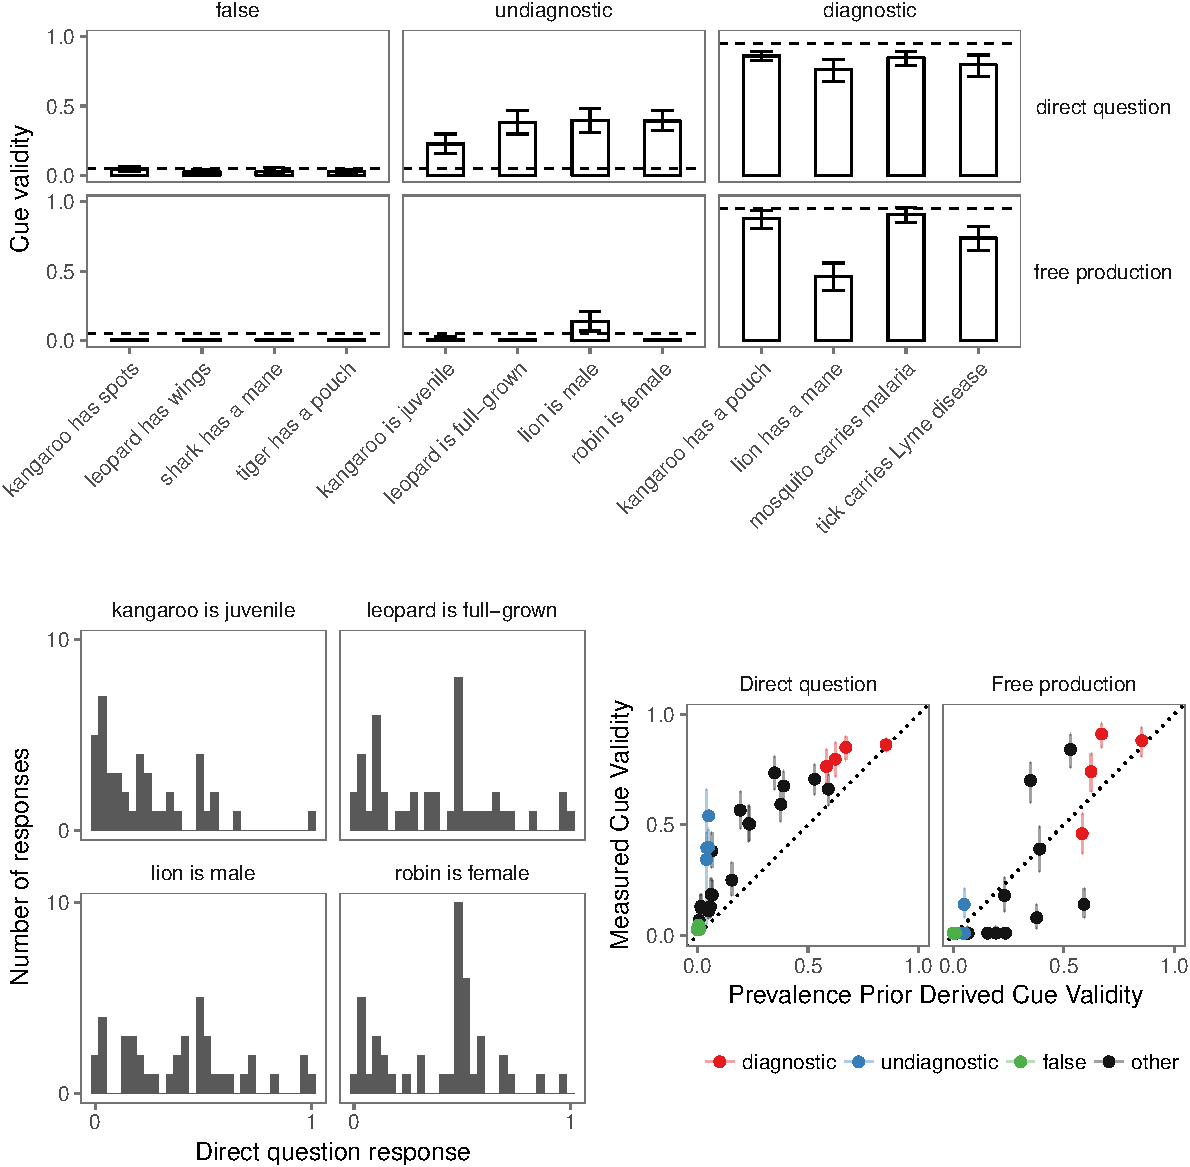
\includegraphics{figs/cv-bothquestions-barplots-1.pdf}
\caption{\label{fig:cv-bothquestions-barplots}Top: Empirically measured cue
validity for two different tasks. Items are grouped by whether the
property is never present in the category (false), the property is
always present in the category and every other category (undiagnostic),
or present in the category and absent from most other categories
(diagnostic). Dotted lines denote theoretical cue validity representing
the desiderata (see text). Error bars denote bootstrapped 95\%
confidence intervals. Bottom left: Raw empirical distributions for
direct question task. Bottom right: Correspondence between measured cue
validity and prevalence prior derived cue validity.}
\end{figure}

\subsection{Comparison with prevalence prior derived cue
validity}\label{comparison-with-prevalence-prior-derived-cue-validity}

To further understand these measures of cue validity, we compare them to
cue validity derived from our prevalence prior elicitation task (Expt.
1a). Expt. 1a is not perfectly designed for this comparison, as we
supplied participants with half of the animal categories that they rated
(the other half was freely generated by participants); including these
supplied categories was important to measure referent-prevalence of
interest (e.g., the percentage of mosquitos that carry malaria).
Including them in this analysis, however, potentially distorts the prior
probability of categories \(P(k)\).

In this analysis, we treat each category entry from Expt. 1a
(participant free production or experimentally supplied category like
mosquitos) as contributing to the prevalence prior. This will result in
the prevalence prior favoring kinds that are easy to produce (like dogs
and cats, which is plausibly a good approximation for \(P(k)\)) as well
as favoring the experimentally supplied kinds (like mosquitos and
robins).

We compute cue validity from the prevalence prior using Bayes' rule.
Figure \ref{fig:cv-bothquestions-barplots} (bottom right) shows the two
measurements of cue validity as they relate to the prevalence prior
derived cue validity. The prevalence prior derived cue validity is
highly associated with both measurements: \(r_{direct}^2(30) = 0.781\);
\(MSE_{direct} = 0.0482\) and \(r_{free}^2(30) = 0.728\);
\(MSE_{free} = 0.0265\). Of primary interest is how the measurements
behave for desiderata items. We see that the prevalence prior derived
cue validity converges with the free production measurement for the
desiderata items (\(r_{free}^2(12) = 0.957\); \(MSE_{free} = 0.00778\)),
whereas the direct question measurement overestimates the cue validity
of undiagnositic features (\(r_{direct}^2(12) = 0.776\);
\(MSE_{direct} = 0.0567\)).

The points of largest deviation for the free-production measurement from
the prevalence prior derived measurement occur where the prevalence
prior derived measure rates the cue validity as relatively high when the
free-production measure gives the item low cue validity (two black
points in Fig. \ref{fig:cv-bothquestions-barplots} (right scatterplot)
high X-value, low Y-value). These two items are: (\enquote{is red},
\enquote{cardinal}) and (\enquote{is white}, \enquote{swan}). These
items should have low relatively cue validity and are overestimated by
the prevalence prior because of the prior on categoryies \(P(k)\) (i.e.,
because they were supplied to every participant and thus get a higher
weighted in the prior for deriving cue validity). In comparison, the
direct question measurement consistently overestimates cue validity
relative to the prevalence prior.

\subsection{Summary}\label{summary}

\emph{Cue validity} is a commonly used measurement for understanding
generic truth conditions. Because we observe different measurements
being used in the literature, we articulated three \emph{a priori}
desiderata to validate a measure of cue validity. We found that the
\enquote{free production} measurement (i.e., having participants
generate categories given a feature), and not the direct question
measurement (i.e., asking participants a likelihood judgment of the
category given the feature), satisfied all three boundary conditions. In
addition, cue validity derived from our prevalence prior measurement
(Expt. 1a) also satisfied these boundary conditions. We conclude that
researchers interested in generic truth conditions should use a free
production paradigm for measuring cue validity.

\newpage

\section{Appendix C: Bayesian Data
Analysis}\label{appendix-c-bayesian-data-analysis}

In our three case studies, we compare an information-theoretic,
computational model of endorsement to human endorsements of
generalizations in language. The model has a single free parameter: the
optimality parameter in Eq. \ref{eq:S1}. Other model parameters
(governing the prevalence prior \(P(h)\) and the referent-prevalence
\(h'\)) are estimated using additional behavioral data (e.g., prior
elicitation tasks). Througout the paper, we model all sources of data
(prevalence prior data, endorsement data) using a single joint-inference
Bayesian data analytic model. In this appendix, we describe this
procedure in more detail for each case study.

\subsection{Modeling prevalence
priors}\label{modeling-prevalence-priors}

In Case Study 1: Generic Language (Expt. 1b), we elicited the prevalence
prior by asking about individual about the prevalence of features for
individual categories. We performed an analagous elicitation in Case
Study 3: Causal Language (Expt. 3a). We describe the analysis using
generics as our running example, but a parallel analysis was done for
causals.

Participants' responses can be thought of as \emph{samples} from the
prevalence prior distribution. Formally, we assume the prior data
(analyzed independently for each property) was generated from one of two
distributions: a distribution corresponding to those kinds with a stable
causal mechanism that \emph{could} give rise to the property
(\(\mathcal{D}_{stable}\)) and a \enquote{transient cause} distribution
corresponding to those kinds without a stable mechanism
(\(\mathcal{D}_{transient}\)). The \enquote{transient} distribution
intuitively corresponds to accidental causes of the feature (e.g., a
lion, who through some genetic mutation, reproduces by laying eggs). We
model this distribution as a Beta distribuition that heavily favors
probabilities near 0:
\(\text{Beta}(\gamma = 0.01, \delta = 100)\).\footnote{Note that we use
  the noncanonical mean \(\gamma\) and concentration \(\xi\) (or,
  inverse-variance) parameterization of the Beta distribution rather
  than the canonical shape (or pseudocount) parameterization for ease of
  posterior inference. The shape parameterization can be recovered
  using: \(\alpha = \gamma \cdot \xi; \beta = (1 - \gamma) \cdot \xi\).}
The \enquote{stable} distribution is modeled as a Beta distribution with
unknown parameters \(\text{Beta}(\gamma, \xi)\).\footnote{Because the
  Beta distribution is not defined at the points 0 and 1, we add
  \(\epsilon\) to the 0 responses and round 1 to 0.99. Similar results
  can be obtained by rounding 0 to 0.01. Alternatively, the
  \enquote{transient} distribution could be defined as a Delta
  distribution at 0, and 0 responses could remain in their raw form.
  Adjusting 1 to \(1- \epsilon\) leads to improper inferences for this
  model, as \(1 - \epsilon\) is only likely under a highly right-skewed
  distribution; treating 1 as \(1- \epsilon\) disproportionately
  influences the shape of \(\mathcal{D}_{stable}\) relative to other
  responses. This problem does not appear for 0 being adjusted to
  \(\epsilon\) because the \enquote{transient} distribution already
  expects such low values.} Finally, we assume that these two components
combine with mixture weighting \(\phi\) such that the data we observe is
\[P(d) = \phi\cdot \text{Beta} (d \mid \gamma, \xi) + (1 -  \phi) \cdot \text{Beta}(d \mid \gamma = 0.01, \xi = 100) \].
We put the following priors over the latent parameters of the model:

\begin{eqnarray*}
\phi_i & \sim & \text{Uniform}(0, 1) \\
\gamma_i & \sim & \text{Uniform}(0, 1) \\
\xi_i & \sim & \text{Uniform}(0, 100)
\end{eqnarray*}

where \(i\) ranges over the different properties (e.g., \emph{lays
eggs}, \emph{carries malaria}).

To learn about the credible values of the parameters, we ran separate
MCMC chains for each item, collecting 75,000 samples, removing the first
25,000 for burn-in. To see how well the mixture model fits the
prevalence prior data, we use the inferred parameters to generate new
data. The data generated from the model's posterior is called the
\emph{posterior predictive distribution} and is an important step in
model criticism. If the model is a good representation of the data, the
posterior predictive data will align with the observed experimental
data. We construct a posterior predictive distribution by
\enquote{forward sampling} the model.\footnote{This can be described by
  the following algorithm: First, flip a coin weighted by \(\phi\). If
  it comes up heads, we then sample from the \enquote{stable} component:
  \(\text{Beta}(\gamma, \xi)\). If it comes up tails, we sample from the
  \enquote{transient} component: \(\text{Beta}(0.01, 100)\). We do this
  many times using the posterior distibution to generate a distribution
  over predicted prevalence ratings.}

In Case Study 2 (Expt. 2a), we asked participants about parameters of
this mixture model (by having participants answer questions abouut
\emph{different kinds of people}) rather than having participants give
samples (e.g., by listing their friends and rating how often their
friends did certain actions). In pilot testing, we found these different
methodologies to give similar results. We made the decision to ask more
abstract information about the events to get at participants' abstract
beliefs about the property rather than their knowledge of true
frequencies. As well, by querying about abstract characters, we were
able to include items that participants might not otherwise feel
comfortable reporting off (e.g., how often their friends smoke
marijuana). The questions used to elicit information about the
parameters are described in the main text.

\subsection{Modeling
referent-prevalence}\label{modeling-referent-prevalence}

In Case Study 1, we used participants prevalence ratings for the
category-of-interest in our generic sentences as the referent-prevalence
that is used in the endorsement model (Eq. \ref{eq:S1}). For a given
generic sentence (e.g., \enquote{Robins lay eggs}), we took the
prevalence ratings for the referent-category (e.g., the percentage of
robins that lay eggs) from the prior elicitation task (Expt. 1b) and
assumed those were generated from a single Beta distribution. We used
the same priors as we did for the \emph{stable cause} component of the
prevalence prior:

\begin{eqnarray*}
\gamma_i & \sim & \text{Uniform}(0, 1) \\
\xi_i & \sim & \text{Uniform}(0, 100)
\end{eqnarray*}

We took samples from the posterior predictive of this Beta distribution
(i.e., reconstructed prevalence ratings) as the
\emph{referent-prevalence} used in the model.

In Expt. 2b (Habitual endorsement), we used the frequency given to
participants in the experimental prompt (e.g., 3 times in the past week)
as the referent-prevalence. In Expt. 2c (\enquote{What is prevalence?}),
we compared two endorsement models that differed in their representation
of referent-prevalence. For one model (past frequency model), it was the
frequency given to participants in the experimental prompt (same as in
Expt. 2b); for the other model (predictive frequency model), we used the
mean elicited frequency from the \emph{predictive frequency} condition
(see main text). In Case Study 3 (Causal endorsement), we used the
proportion of successful causal events given to participants in the
experimental prompt (e.g., 70 out of 100 uses of Herb C made animals
sleepy).

\subsection{Jointly modeling referent-prevalence, prevalence priors, and
generic
endorsements}\label{jointly-modeling-referent-prevalence-prevalence-priors-and-generic-endorsements}

To fit the generic endorsement models, we incorporate them into the
Bayesian data analytic model of the prevalence prior data (described
above) to create a single, joint-inference model where the optimality
parameter \(\lambda_1\) (Eq. \ref{eq:S1}) is inferred jointly with all
the other latent parameters of the full model (the referent-prevalence
\(h'_{k, f}\) for each category \(k\) and property \(f\) and the
parameters of the prevalence priors \(P_f(h)\) for each property \(f\))
using data from Expt. 1a \& b (Figure \ref{fig:genericsModelDiagram}).
For the parameters of the prevalence prior distributions, we use the
same priors described in Expt. 1b; for the speaker optimality parameter,
we use a prior with a range consistent with previous literature using
the same model class: \(\lambda_1 \sim \text{Uniform}(0,5)\). We learn
about the \emph{a posteriori} credible values of the joint inference
models by collecting samples from 3 MCMC chains of 100,000 iterations
removing the first 50,000 iterations for burn-in, using an
incrementalized version of the Metropolis-Hastings algorithm (Ritchie et
al., 2016).

\begin{figure}[htbp]
\centering
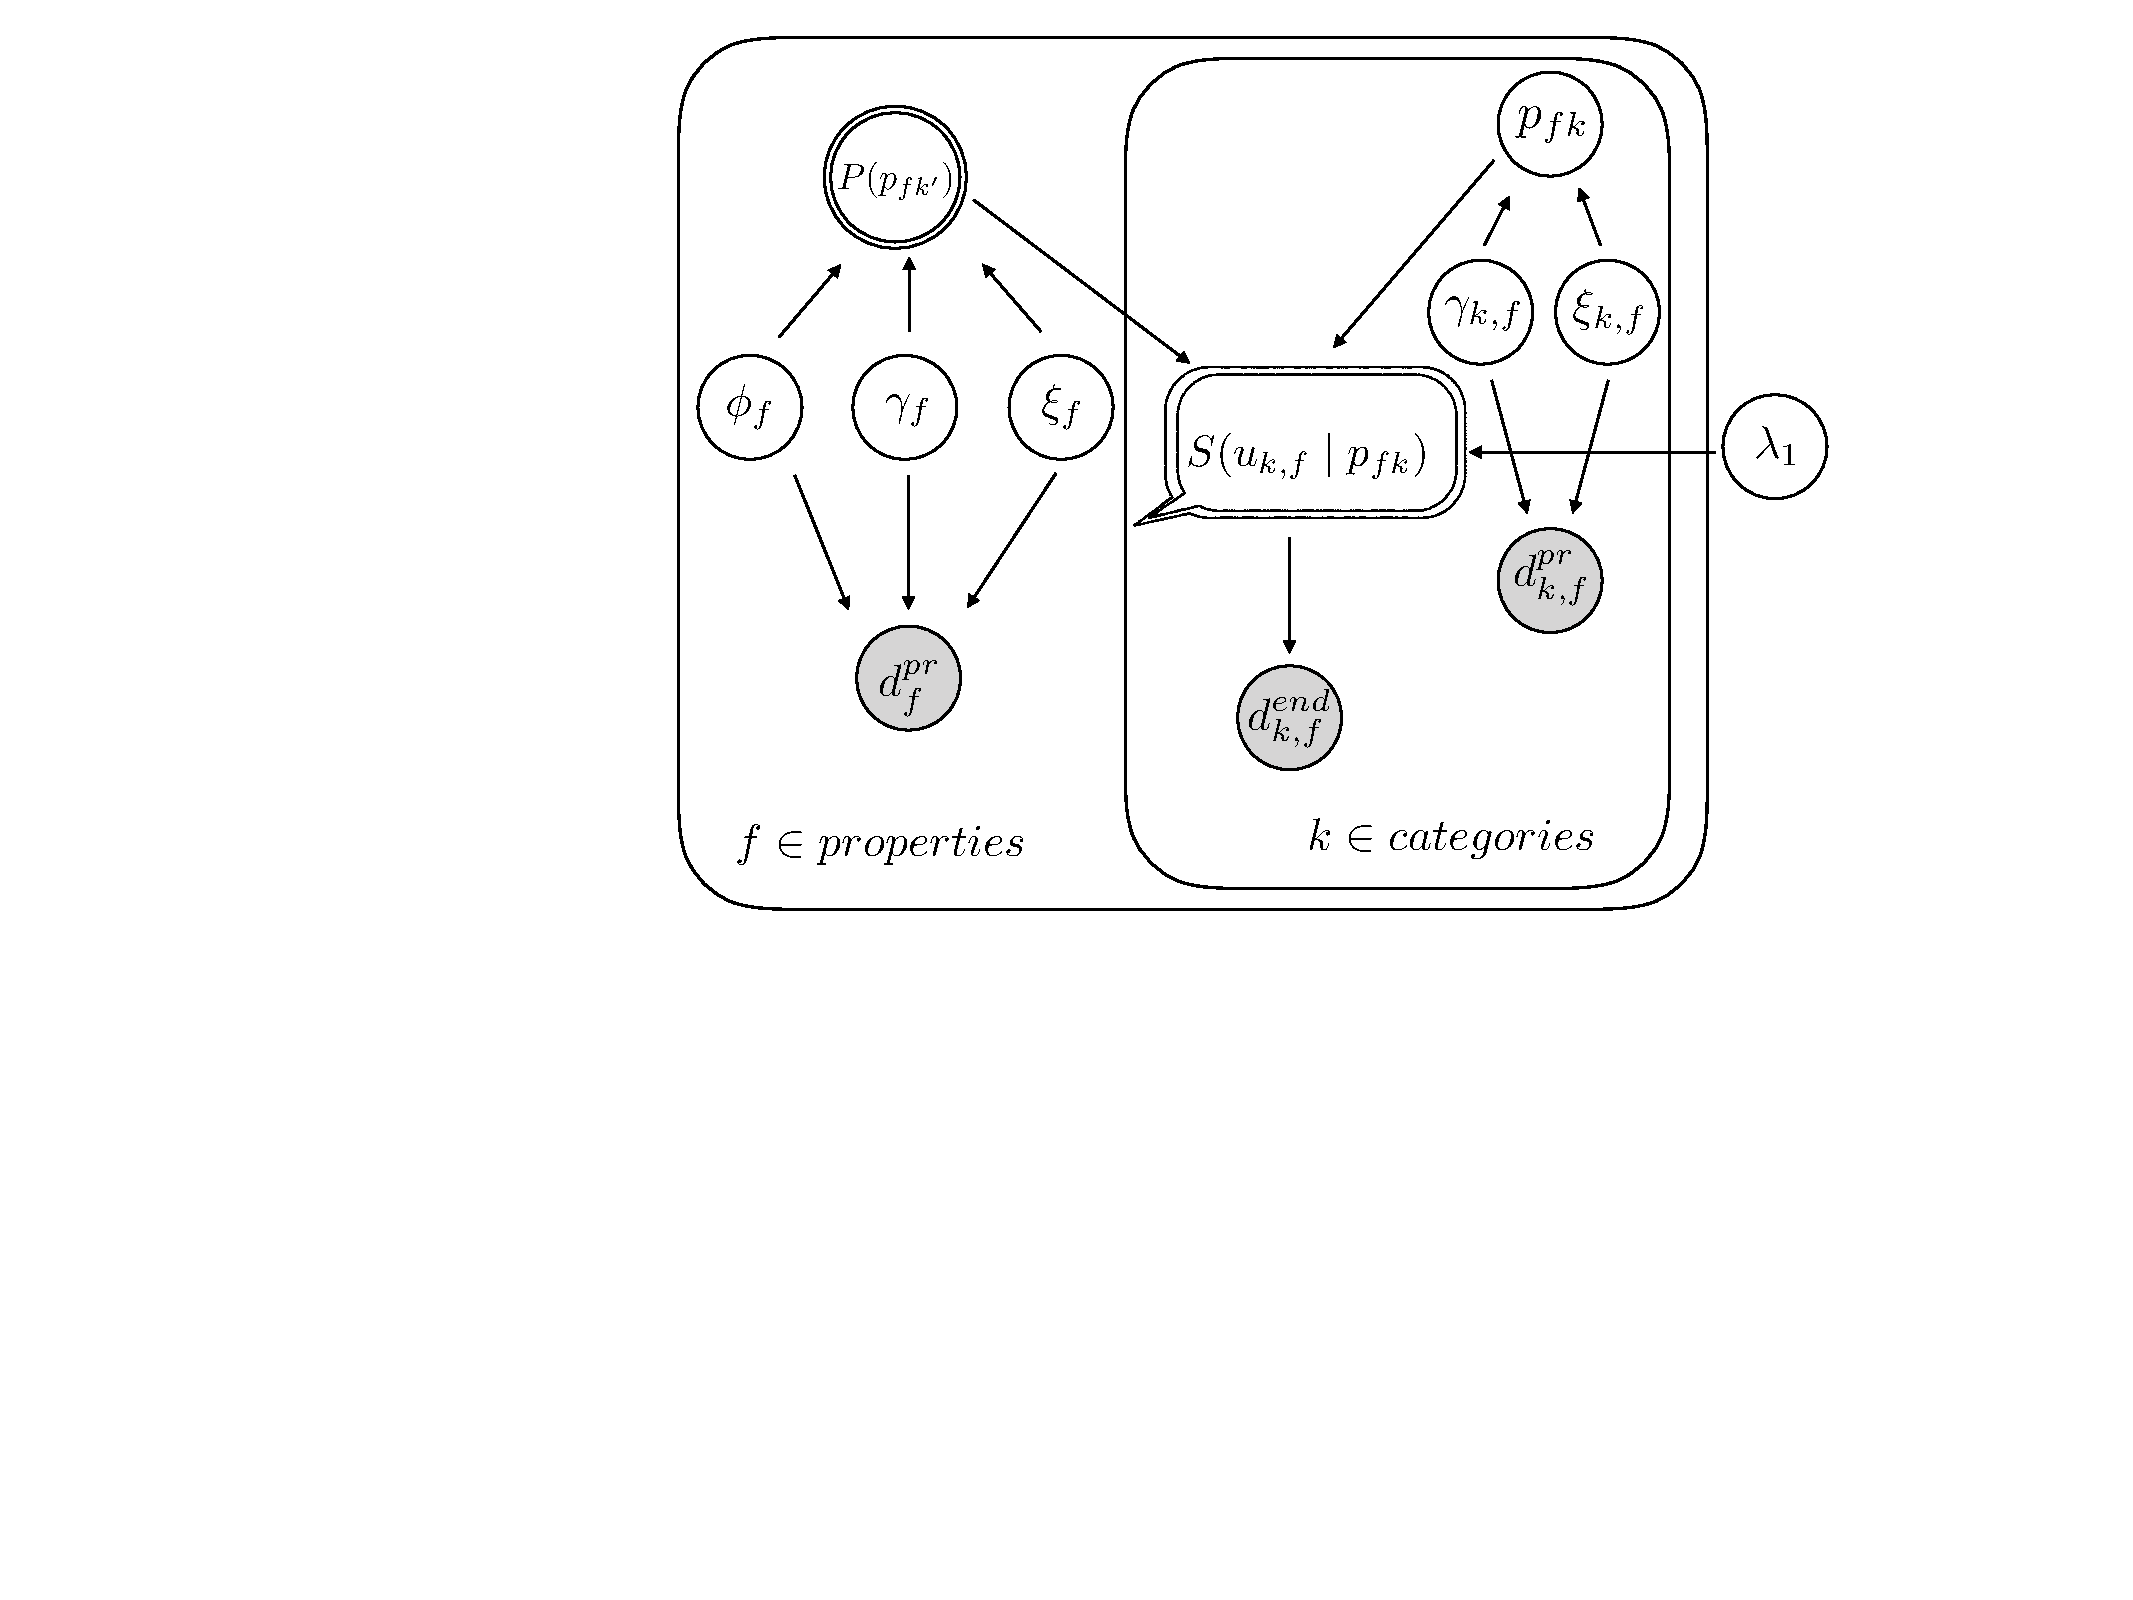
\includegraphics{figs/generics_bayesnetmodel.pdf}
\caption{\label{fig:genericsModelDiagram}Graphical model corresponding to
the fully Bayesian data analysis of the RSA model. The prevalence prior
data \(d^{pr}_{f}\) is assumed to be generated from the mixture model
validated in Expt. 1a. The referent-category prevalence \(d^{pr}_{k,f}\)
is generated from a latent prevalence \(p_{fk}\). The fixed-threshold
(control model) or uncertain-threshold model take the prevalence priors
\(P_f(h)\), the referent-prevalence \(h\), and a single speaker
optimality parameter \(\lambda\) as input. This overall structured is
repeated (except \(\lambda\)) for each of the unique properties \(f\)
and categories \(k\) that correspond to the generic sentences in our
stimulus set. Note that S corresponds to a probabilistic \emph{function}
and not a \emph{random variable} that is standard in graphical model
notation; S cannot be represented by a graphical model because it has
recursion.}
\end{figure}

In addition to examining the posterior predictive distribution on
endorsement judgments (presented in main text), we examined the marginal
posteriors on parameters of the prevalence priors and
referent-prevalence. These marginal distributions are important to
examine to confirm that they have not changed significantly from the
parameters inferred from their private data sources in isolation. For
example, when modeling the referent-prevalence data in isolation, the
model infers that roughly 50\% of robins lay eggs, as that is what
participants tend to say in the prevalence elicitation task.\footnote{Some
  participants do report that 100\% of robins lay eggs so the average
  prevalence rating is closer to 65\%..}. The question for this joint
inference model is whether or not it still believes that roughly 50\% of
robins lay eggs. We found that the referent-prevalences and prevalence
priors inferred under the joint model were almost indistinguishable from
those inferred using only their data, suggesting that the modeling all
three data sources together does not come at the cost of modeling any
one of them accurately.






\end{document}
